\documentclass[twoside]{book}

% Packages required by doxygen
\usepackage{fixltx2e}
\usepackage{calc}
\usepackage{doxygen}
\usepackage{graphicx}
\usepackage[utf8]{inputenc}
\usepackage{makeidx}
\usepackage{multicol}
\usepackage{multirow}
\PassOptionsToPackage{warn}{textcomp}
\usepackage{textcomp}
\usepackage[nointegrals]{wasysym}
\usepackage[table]{xcolor}

% Font selection
\usepackage[T1]{fontenc}
\usepackage{mathptmx}
\usepackage[scaled=.90]{helvet}
\usepackage{courier}
\usepackage{amssymb}
\usepackage{sectsty}
\renewcommand{\familydefault}{\sfdefault}
\allsectionsfont{%
  \fontseries{bc}\selectfont%
  \color{darkgray}%
}
\renewcommand{\DoxyLabelFont}{%
  \fontseries{bc}\selectfont%
  \color{darkgray}%
}
\newcommand{\+}{\discretionary{\mbox{\scriptsize$\hookleftarrow$}}{}{}}

% Page & text layout
\usepackage{geometry}
\geometry{%
  a4paper,%
  top=2.5cm,%
  bottom=2.5cm,%
  left=2.5cm,%
  right=2.5cm%
}
\tolerance=750
\hfuzz=15pt
\hbadness=750
\setlength{\emergencystretch}{15pt}
\setlength{\parindent}{0cm}
\setlength{\parskip}{0.2cm}
\makeatletter
\renewcommand{\paragraph}{%
  \@startsection{paragraph}{4}{0ex}{-1.0ex}{1.0ex}{%
    \normalfont\normalsize\bfseries\SS@parafont%
  }%
}
\renewcommand{\subparagraph}{%
  \@startsection{subparagraph}{5}{0ex}{-1.0ex}{1.0ex}{%
    \normalfont\normalsize\bfseries\SS@subparafont%
  }%
}
\makeatother

% Headers & footers
\usepackage{fancyhdr}
\pagestyle{fancyplain}
\fancyhead[LE]{\fancyplain{}{\bfseries\thepage}}
\fancyhead[CE]{\fancyplain{}{}}
\fancyhead[RE]{\fancyplain{}{\bfseries\leftmark}}
\fancyhead[LO]{\fancyplain{}{\bfseries\rightmark}}
\fancyhead[CO]{\fancyplain{}{}}
\fancyhead[RO]{\fancyplain{}{\bfseries\thepage}}
\fancyfoot[LE]{\fancyplain{}{}}
\fancyfoot[CE]{\fancyplain{}{}}
\fancyfoot[RE]{\fancyplain{}{\bfseries\scriptsize Generated on Thu Oct 2 2014 14\+:57\+:29 for 0x\+Socket by Doxygen }}
\fancyfoot[LO]{\fancyplain{}{\bfseries\scriptsize Generated on Thu Oct 2 2014 14\+:57\+:29 for 0x\+Socket by Doxygen }}
\fancyfoot[CO]{\fancyplain{}{}}
\fancyfoot[RO]{\fancyplain{}{}}
\renewcommand{\footrulewidth}{0.4pt}
\renewcommand{\chaptermark}[1]{%
  \markboth{#1}{}%
}
\renewcommand{\sectionmark}[1]{%
  \markright{\thesection\ #1}%
}

% Indices & bibliography
\usepackage{natbib}
\usepackage[titles]{tocloft}
\setcounter{tocdepth}{3}
\setcounter{secnumdepth}{5}
\makeindex

% Hyperlinks (required, but should be loaded last)
\usepackage{ifpdf}
\ifpdf
  \usepackage[pdftex,pagebackref=true]{hyperref}
\else
  \usepackage[ps2pdf,pagebackref=true]{hyperref}
\fi
\hypersetup{%
  colorlinks=true,%
  linkcolor=blue,%
  citecolor=blue,%
  unicode%
}

% Custom commands
\newcommand{\clearemptydoublepage}{%
  \newpage{\pagestyle{empty}\cleardoublepage}%
}


%===== C O N T E N T S =====

\begin{document}

% Titlepage & ToC
\hypersetup{pageanchor=false,
             bookmarks=true,
             bookmarksnumbered=true,
             pdfencoding=unicode
            }
\pagenumbering{roman}
\begin{titlepage}
\vspace*{7cm}
\begin{center}%
{\Large 0x\+Socket \\[1ex]\large 0.\+2 }\\
\vspace*{1cm}
{\large Generated by Doxygen 1.8.8}\\
\vspace*{0.5cm}
{\small Thu Oct 2 2014 14:57:29}\\
\end{center}
\end{titlepage}
\clearemptydoublepage
\tableofcontents
\clearemptydoublepage
\pagenumbering{arabic}
\hypersetup{pageanchor=true}

%--- Begin generated contents ---
\chapter{Hierarchical Index}
\section{Class Hierarchy}
This inheritance list is sorted roughly, but not completely, alphabetically\+:\begin{DoxyCompactList}
\item \contentsline{section}{Server\+Socket}{\pageref{classServerSocket}}{}
\begin{DoxyCompactList}
\item \contentsline{section}{T\+C\+P\+Server\+Socket}{\pageref{classTCPServerSocket}}{}
\item \contentsline{section}{U\+N\+I\+X\+Server\+Socket}{\pageref{classUNIXServerSocket}}{}
\end{DoxyCompactList}
\item \contentsline{section}{Socket\+Fd}{\pageref{classSocketFd}}{}
\begin{DoxyCompactList}
\item \contentsline{section}{Connection}{\pageref{classConnection}}{}
\begin{DoxyCompactList}
\item \contentsline{section}{T\+C\+P\+Client\+Socket}{\pageref{classTCPClientSocket}}{}
\item \contentsline{section}{U\+N\+I\+X\+Client\+Socket}{\pageref{classUNIXClientSocket}}{}
\end{DoxyCompactList}
\item \contentsline{section}{T\+C\+P\+Server\+Socket}{\pageref{classTCPServerSocket}}{}
\item \contentsline{section}{U\+D\+P\+Socket}{\pageref{classUDPSocket}}{}
\begin{DoxyCompactList}
\item \contentsline{section}{U\+D\+P\+Client\+Socket}{\pageref{classUDPClientSocket}}{}
\item \contentsline{section}{U\+D\+P\+Server\+Socket}{\pageref{classUDPServerSocket}}{}
\end{DoxyCompactList}
\item \contentsline{section}{U\+N\+I\+X\+Server\+Socket}{\pageref{classUNIXServerSocket}}{}
\end{DoxyCompactList}
\item \contentsline{section}{T\+C\+P\+Socket}{\pageref{classTCPSocket}}{}
\begin{DoxyCompactList}
\item \contentsline{section}{T\+C\+P\+Client\+Socket}{\pageref{classTCPClientSocket}}{}
\item \contentsline{section}{T\+C\+P\+Server\+Socket}{\pageref{classTCPServerSocket}}{}
\end{DoxyCompactList}
\item \contentsline{section}{Transceiver}{\pageref{classTransceiver}}{}
\begin{DoxyCompactList}
\item \contentsline{section}{Connection}{\pageref{classConnection}}{}
\item \contentsline{section}{U\+D\+P\+Socket}{\pageref{classUDPSocket}}{}
\end{DoxyCompactList}
\end{DoxyCompactList}

\chapter{Class Index}
\section{Class List}
Here are the classes, structs, unions and interfaces with brief descriptions\+:\begin{DoxyCompactList}
\item\contentsline{section}{\hyperlink{classConnection}{Connection} }{\pageref{classConnection}}{}
\item\contentsline{section}{\hyperlink{classServerSocket}{Server\+Socket} \\*Not instanziable Base\+Class for all \hyperlink{classServerSocket}{Server\+Socket} Classes }{\pageref{classServerSocket}}{}
\item\contentsline{section}{\hyperlink{classSocketFd}{Socket\+Fd} \\*Not initalizable Base\+Class for Socket\+File\+Descriptor }{\pageref{classSocketFd}}{}
\item\contentsline{section}{\hyperlink{classTCPClientSocket}{T\+C\+P\+Client\+Socket} }{\pageref{classTCPClientSocket}}{}
\item\contentsline{section}{\hyperlink{classTCPServerSocket}{T\+C\+P\+Server\+Socket} }{\pageref{classTCPServerSocket}}{}
\item\contentsline{section}{\hyperlink{classTCPSocket}{T\+C\+P\+Socket} }{\pageref{classTCPSocket}}{}
\item\contentsline{section}{\hyperlink{classTransceiver}{Transceiver} }{\pageref{classTransceiver}}{}
\item\contentsline{section}{\hyperlink{classUDPClientSocket}{U\+D\+P\+Client\+Socket} }{\pageref{classUDPClientSocket}}{}
\item\contentsline{section}{\hyperlink{classUDPServerSocket}{U\+D\+P\+Server\+Socket} }{\pageref{classUDPServerSocket}}{}
\item\contentsline{section}{\hyperlink{classUDPSocket}{U\+D\+P\+Socket} }{\pageref{classUDPSocket}}{}
\item\contentsline{section}{\hyperlink{classUNIXClientSocket}{U\+N\+I\+X\+Client\+Socket} }{\pageref{classUNIXClientSocket}}{}
\item\contentsline{section}{\hyperlink{classUNIXServerSocket}{U\+N\+I\+X\+Server\+Socket} }{\pageref{classUNIXServerSocket}}{}
\end{DoxyCompactList}

\chapter{File Index}
\section{File List}
Here is a list of all files with brief descriptions\+:\begin{DoxyCompactList}
\item\contentsline{section}{include/\hyperlink{Connection_8h}{Connection.\+h} }{\pageref{Connection_8h}}{}
\item\contentsline{section}{include/\hyperlink{ServerSocket_8h}{Server\+Socket.\+h} }{\pageref{ServerSocket_8h}}{}
\item\contentsline{section}{include/\hyperlink{Socket_8h}{Socket.\+h} }{\pageref{Socket_8h}}{}
\item\contentsline{section}{include/\hyperlink{SocketFd_8h}{Socket\+Fd.\+h} }{\pageref{SocketFd_8h}}{}
\item\contentsline{section}{include/\hyperlink{TCPClientSocket_8h}{T\+C\+P\+Client\+Socket.\+h} }{\pageref{TCPClientSocket_8h}}{}
\item\contentsline{section}{include/\hyperlink{TCPServerSocket_8h}{T\+C\+P\+Server\+Socket.\+h} }{\pageref{TCPServerSocket_8h}}{}
\item\contentsline{section}{include/\hyperlink{TCPSocket_8h}{T\+C\+P\+Socket.\+h} }{\pageref{TCPSocket_8h}}{}
\item\contentsline{section}{include/\hyperlink{Transceiver_8h}{Transceiver.\+h} }{\pageref{Transceiver_8h}}{}
\item\contentsline{section}{include/\hyperlink{UDPClientSocket_8h}{U\+D\+P\+Client\+Socket.\+h} }{\pageref{UDPClientSocket_8h}}{}
\item\contentsline{section}{include/\hyperlink{UDPServerSocket_8h}{U\+D\+P\+Server\+Socket.\+h} }{\pageref{UDPServerSocket_8h}}{}
\item\contentsline{section}{include/\hyperlink{UDPSocket_8h}{U\+D\+P\+Socket.\+h} }{\pageref{UDPSocket_8h}}{}
\item\contentsline{section}{include/\hyperlink{UNIXClientSocket_8h}{U\+N\+I\+X\+Client\+Socket.\+h} }{\pageref{UNIXClientSocket_8h}}{}
\item\contentsline{section}{include/\hyperlink{UNIXServerSocket_8h}{U\+N\+I\+X\+Server\+Socket.\+h} }{\pageref{UNIXServerSocket_8h}}{}
\item\contentsline{section}{src/\hyperlink{Connection_8cpp}{Connection.\+cpp} }{\pageref{Connection_8cpp}}{}
\item\contentsline{section}{src/\hyperlink{Example_8cpp}{Example.\+cpp} }{\pageref{Example_8cpp}}{}
\item\contentsline{section}{src/\hyperlink{ServerSocket_8cpp}{Server\+Socket.\+cpp} }{\pageref{ServerSocket_8cpp}}{}
\item\contentsline{section}{src/\hyperlink{SocketFd_8cpp}{Socket\+Fd.\+cpp} }{\pageref{SocketFd_8cpp}}{}
\item\contentsline{section}{src/\hyperlink{TCPClientSocket_8cpp}{T\+C\+P\+Client\+Socket.\+cpp} }{\pageref{TCPClientSocket_8cpp}}{}
\item\contentsline{section}{src/\hyperlink{TCPServerSocket_8cpp}{T\+C\+P\+Server\+Socket.\+cpp} }{\pageref{TCPServerSocket_8cpp}}{}
\item\contentsline{section}{src/\hyperlink{TCPSocket_8cpp}{T\+C\+P\+Socket.\+cpp} }{\pageref{TCPSocket_8cpp}}{}
\item\contentsline{section}{src/\hyperlink{Transceiver_8cpp}{Transceiver.\+cpp} }{\pageref{Transceiver_8cpp}}{}
\item\contentsline{section}{src/\hyperlink{UDPClientSocket_8cpp}{U\+D\+P\+Client\+Socket.\+cpp} }{\pageref{UDPClientSocket_8cpp}}{}
\item\contentsline{section}{src/\hyperlink{UDPServerSocket_8cpp}{U\+D\+P\+Server\+Socket.\+cpp} }{\pageref{UDPServerSocket_8cpp}}{}
\item\contentsline{section}{src/\hyperlink{UDPSocket_8cpp}{U\+D\+P\+Socket.\+cpp} }{\pageref{UDPSocket_8cpp}}{}
\item\contentsline{section}{src/\hyperlink{UNIXClientSocket_8cpp}{U\+N\+I\+X\+Client\+Socket.\+cpp} }{\pageref{UNIXClientSocket_8cpp}}{}
\item\contentsline{section}{src/\hyperlink{UNIXServerSocket_8cpp}{U\+N\+I\+X\+Server\+Socket.\+cpp} }{\pageref{UNIXServerSocket_8cpp}}{}
\end{DoxyCompactList}

\chapter{Class Documentation}
\hypertarget{classConnection}{\section{Connection Class Reference}
\label{classConnection}\index{Connection@{Connection}}
}


{\ttfamily \#include $<$Connection.\+h$>$}



Inheritance diagram for Connection\+:
\nopagebreak
\begin{figure}[H]
\begin{center}
\leavevmode
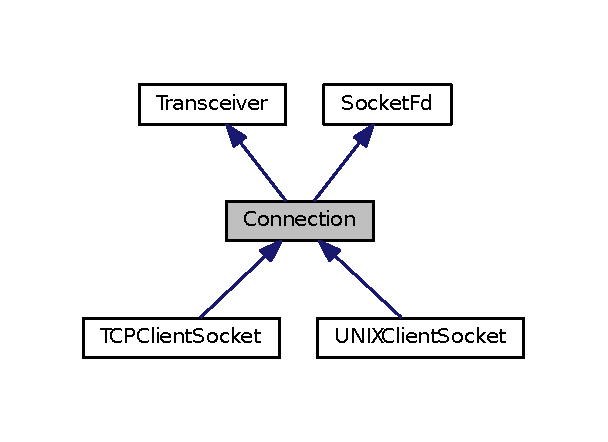
\includegraphics[width=292pt]{classConnection__inherit__graph}
\end{center}
\end{figure}


Collaboration diagram for Connection\+:
\nopagebreak
\begin{figure}[H]
\begin{center}
\leavevmode
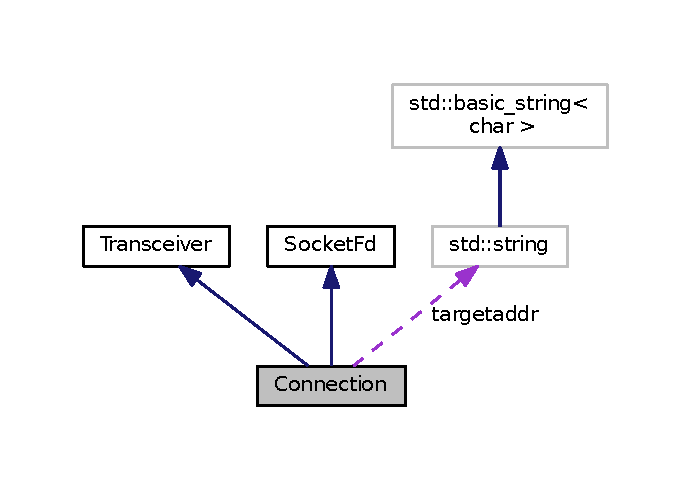
\includegraphics[width=332pt]{classConnection__coll__graph}
\end{center}
\end{figure}
\subsection*{Public Member Functions}
\begin{DoxyCompactItemize}
\item 
\hyperlink{classConnection_a3bc70a7fdfcabe58f6ca003f450e7b34}{Connection} (const int=0, const std\+::string taddr=\char`\"{}\char`\"{})
\item 
virtual \hyperlink{classConnection_a2e4352edf667bea83001569e9da8a24d}{$\sim$\+Connection} ()
\item 
int \hyperlink{classConnection_ab16b8a780c69303beec9b1f67fb596f3}{recv} (char $\ast$, const unsigned, const int=-\/1)
\item 
int \hyperlink{classConnection_a5466a66e569e81d891559686f2c7594b}{send} (const char $\ast$, const unsigned, const int=-\/1)
\end{DoxyCompactItemize}
\subsection*{Public Attributes}
\begin{DoxyCompactItemize}
\item 
std\+::string \hyperlink{classConnection_a04bb846a50a9357bab86238956940d65}{targetaddr}
\end{DoxyCompactItemize}
\subsection*{Private Member Functions}
\begin{DoxyCompactItemize}
\item 
int \hyperlink{classConnection_a4e186a7e69d56c0bb84ef56032b89427}{\+\_\+poll} (const int=-\/1)
\end{DoxyCompactItemize}
\subsection*{Private Attributes}
\begin{DoxyCompactItemize}
\item 
int \hyperlink{classConnection_af54be737cc02308299c2e80a893a3e46}{n}
\item 
unsigned int \hyperlink{classConnection_aca989af92a96ac113222d7b8640df507}{sum}
\end{DoxyCompactItemize}
\subsection*{Additional Inherited Members}


\subsection{Detailed Description}


Definition at line 13 of file Connection.\+h.



\subsection{Constructor \& Destructor Documentation}
\hypertarget{classConnection_a3bc70a7fdfcabe58f6ca003f450e7b34}{\index{Connection@{Connection}!Connection@{Connection}}
\index{Connection@{Connection}!Connection@{Connection}}
\subsubsection[{Connection}]{\setlength{\rightskip}{0pt plus 5cm}Connection\+::\+Connection (
\begin{DoxyParamCaption}
\item[{const int}]{fd = {\ttfamily 0}, }
\item[{const std\+::string}]{taddr = {\ttfamily \char`\"{}\char`\"{}}}
\end{DoxyParamCaption}
)}}\label{classConnection_a3bc70a7fdfcabe58f6ca003f450e7b34}


Definition at line 3 of file Connection.\+cpp.



References n, sum, targetaddr, and Socket\+Fd\+::ufds.

\hypertarget{classConnection_a2e4352edf667bea83001569e9da8a24d}{\index{Connection@{Connection}!````~Connection@{$\sim$\+Connection}}
\index{````~Connection@{$\sim$\+Connection}!Connection@{Connection}}
\subsubsection[{$\sim$\+Connection}]{\setlength{\rightskip}{0pt plus 5cm}Connection\+::$\sim$\+Connection (
\begin{DoxyParamCaption}
{}
\end{DoxyParamCaption}
)\hspace{0.3cm}{\ttfamily [virtual]}}}\label{classConnection_a2e4352edf667bea83001569e9da8a24d}


Definition at line 10 of file Connection.\+cpp.



\subsection{Member Function Documentation}
\hypertarget{classConnection_a4e186a7e69d56c0bb84ef56032b89427}{\index{Connection@{Connection}!\+\_\+poll@{\+\_\+poll}}
\index{\+\_\+poll@{\+\_\+poll}!Connection@{Connection}}
\subsubsection[{\+\_\+poll}]{\setlength{\rightskip}{0pt plus 5cm}int Connection\+::\+\_\+poll (
\begin{DoxyParamCaption}
\item[{const int}]{msec = {\ttfamily -\/1}}
\end{DoxyParamCaption}
)\hspace{0.3cm}{\ttfamily [private]}}}\label{classConnection_a4e186a7e69d56c0bb84ef56032b89427}


Definition at line 42 of file Connection.\+cpp.



References Socket\+Fd\+::ufds.



Referenced by recv(), and send().



Here is the caller graph for this function\+:
\nopagebreak
\begin{figure}[H]
\begin{center}
\leavevmode
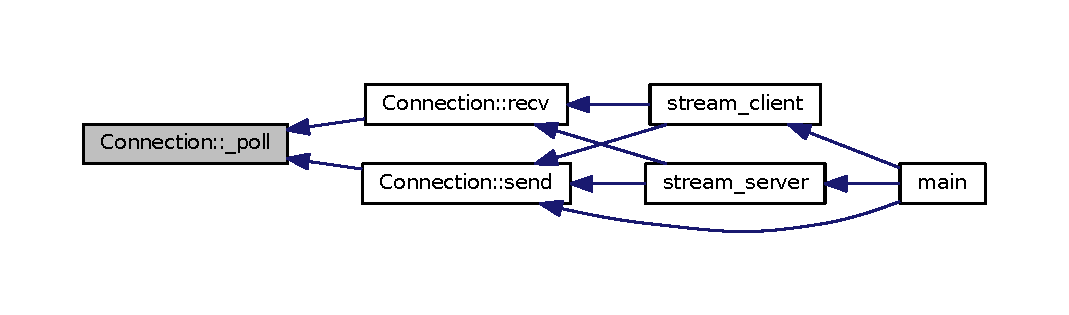
\includegraphics[width=350pt]{classConnection_a4e186a7e69d56c0bb84ef56032b89427_icgraph}
\end{center}
\end{figure}


\hypertarget{classConnection_ab16b8a780c69303beec9b1f67fb596f3}{\index{Connection@{Connection}!recv@{recv}}
\index{recv@{recv}!Connection@{Connection}}
\subsubsection[{recv}]{\setlength{\rightskip}{0pt plus 5cm}int Connection\+::recv (
\begin{DoxyParamCaption}
\item[{char $\ast$}]{buf, }
\item[{const unsigned}]{size, }
\item[{const int}]{msec = {\ttfamily -\/1}}
\end{DoxyParamCaption}
)\hspace{0.3cm}{\ttfamily [virtual]}}}\label{classConnection_ab16b8a780c69303beec9b1f67fb596f3}


Implements \hyperlink{classTransceiver_aef7153a423766522f4f82c1300157048}{Transceiver}.



Definition at line 35 of file Connection.\+cpp.



References \+\_\+poll(), and W\+E\+A\+D\+M\+A\+C\+R\+O.



Referenced by stream\+\_\+client(), and stream\+\_\+server().



Here is the call graph for this function\+:
\nopagebreak
\begin{figure}[H]
\begin{center}
\leavevmode
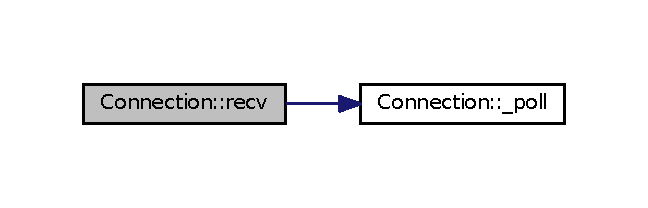
\includegraphics[width=311pt]{classConnection_ab16b8a780c69303beec9b1f67fb596f3_cgraph}
\end{center}
\end{figure}




Here is the caller graph for this function\+:
\nopagebreak
\begin{figure}[H]
\begin{center}
\leavevmode
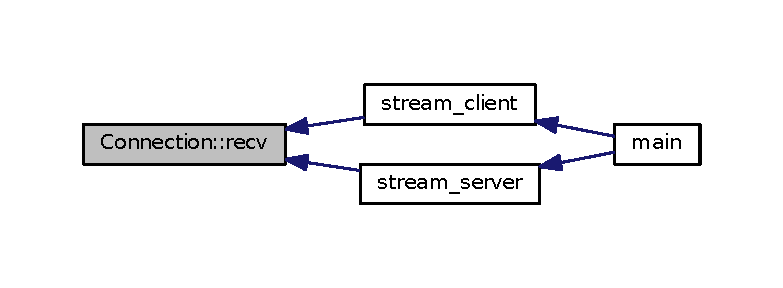
\includegraphics[width=350pt]{classConnection_ab16b8a780c69303beec9b1f67fb596f3_icgraph}
\end{center}
\end{figure}


\hypertarget{classConnection_a5466a66e569e81d891559686f2c7594b}{\index{Connection@{Connection}!send@{send}}
\index{send@{send}!Connection@{Connection}}
\subsubsection[{send}]{\setlength{\rightskip}{0pt plus 5cm}int Connection\+::send (
\begin{DoxyParamCaption}
\item[{const char $\ast$}]{buf, }
\item[{const unsigned}]{size, }
\item[{const int}]{msec = {\ttfamily -\/1}}
\end{DoxyParamCaption}
)\hspace{0.3cm}{\ttfamily [virtual]}}}\label{classConnection_a5466a66e569e81d891559686f2c7594b}


Implements \hyperlink{classTransceiver_aa54935e0032d9ab6c531024e001ae19d}{Transceiver}.



Definition at line 30 of file Connection.\+cpp.



References \+\_\+poll(), and W\+E\+A\+D\+M\+A\+C\+R\+O.



Referenced by main(), stream\+\_\+client(), and stream\+\_\+server().



Here is the call graph for this function\+:
\nopagebreak
\begin{figure}[H]
\begin{center}
\leavevmode
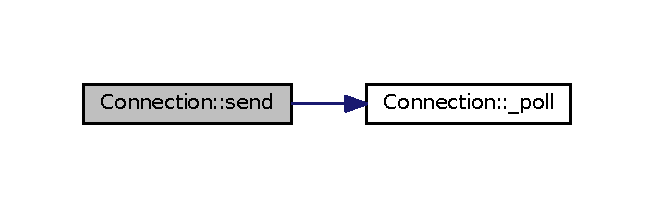
\includegraphics[width=314pt]{classConnection_a5466a66e569e81d891559686f2c7594b_cgraph}
\end{center}
\end{figure}




Here is the caller graph for this function\+:
\nopagebreak
\begin{figure}[H]
\begin{center}
\leavevmode
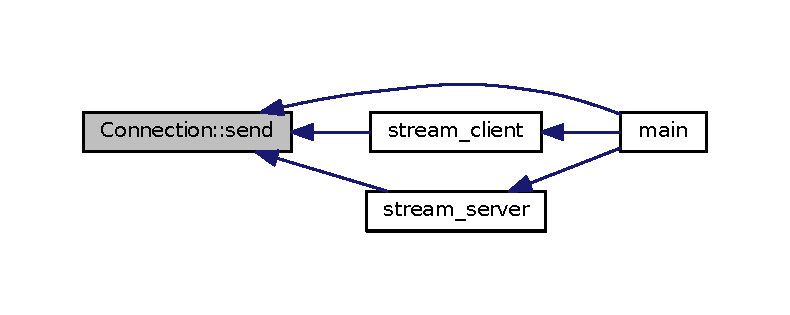
\includegraphics[width=350pt]{classConnection_a5466a66e569e81d891559686f2c7594b_icgraph}
\end{center}
\end{figure}




\subsection{Member Data Documentation}
\hypertarget{classConnection_af54be737cc02308299c2e80a893a3e46}{\index{Connection@{Connection}!n@{n}}
\index{n@{n}!Connection@{Connection}}
\subsubsection[{n}]{\setlength{\rightskip}{0pt plus 5cm}int Connection\+::n\hspace{0.3cm}{\ttfamily [private]}}}\label{classConnection_af54be737cc02308299c2e80a893a3e46}


Definition at line 17 of file Connection.\+h.



Referenced by Connection(), and T\+C\+P\+Client\+Socket\+::\+T\+C\+P\+Client\+Socket().

\hypertarget{classConnection_aca989af92a96ac113222d7b8640df507}{\index{Connection@{Connection}!sum@{sum}}
\index{sum@{sum}!Connection@{Connection}}
\subsubsection[{sum}]{\setlength{\rightskip}{0pt plus 5cm}unsigned int Connection\+::sum\hspace{0.3cm}{\ttfamily [private]}}}\label{classConnection_aca989af92a96ac113222d7b8640df507}


Definition at line 18 of file Connection.\+h.



Referenced by Connection().

\hypertarget{classConnection_a04bb846a50a9357bab86238956940d65}{\index{Connection@{Connection}!targetaddr@{targetaddr}}
\index{targetaddr@{targetaddr}!Connection@{Connection}}
\subsubsection[{targetaddr}]{\setlength{\rightskip}{0pt plus 5cm}std\+::string Connection\+::targetaddr}}\label{classConnection_a04bb846a50a9357bab86238956940d65}


Definition at line 22 of file Connection.\+h.



Referenced by Connection(), and T\+C\+P\+Client\+Socket\+::\+T\+C\+P\+Client\+Socket().



The documentation for this class was generated from the following files\+:\begin{DoxyCompactItemize}
\item 
include/\hyperlink{Connection_8h}{Connection.\+h}\item 
src/\hyperlink{Connection_8cpp}{Connection.\+cpp}\end{DoxyCompactItemize}

\hypertarget{classServerSocket}{\section{Server\+Socket Class Reference}
\label{classServerSocket}\index{Server\+Socket@{Server\+Socket}}
}


Not instanziable Base\+Class for all \hyperlink{classServerSocket}{Server\+Socket} Classes.  




{\ttfamily \#include $<$Server\+Socket.\+h$>$}



Inheritance diagram for Server\+Socket\+:
\nopagebreak
\begin{figure}[H]
\begin{center}
\leavevmode
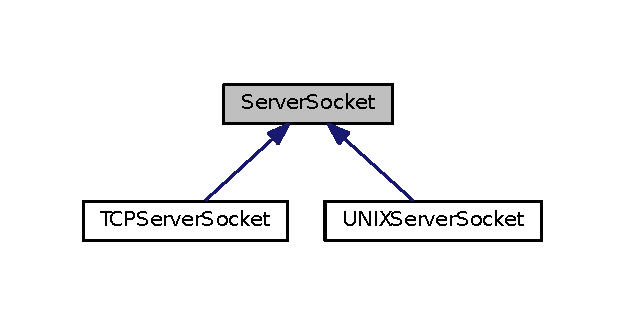
\includegraphics[width=300pt]{classServerSocket__inherit__graph}
\end{center}
\end{figure}
\subsection*{Public Member Functions}
\begin{DoxyCompactItemize}
\item 
virtual \hyperlink{classServerSocket_a510674d924c2544e6b0069e39c36516b}{$\sim$\+Server\+Socket} ()
\item 
virtual \hyperlink{classConnection}{Connection} $\ast$ \hyperlink{classServerSocket_a1d7054bc388f2d789d2124dd96939d90}{accept} ()=0
\end{DoxyCompactItemize}
\subsection*{Protected Member Functions}
\begin{DoxyCompactItemize}
\item 
\hyperlink{classServerSocket_a2b3098589541243241ca25495155186c}{Server\+Socket} ()
\end{DoxyCompactItemize}


\subsection{Detailed Description}
Not instanziable Base\+Class for all \hyperlink{classServerSocket}{Server\+Socket} Classes. 

Not instanziable Base\+Class for all \hyperlink{classServerSocket}{Server\+Socket} Classes. Must provides an \hyperlink{classServerSocket_a1d7054bc388f2d789d2124dd96939d90}{accept()} function that will return a \hyperlink{classConnection}{Connection} Object 

Definition at line 11 of file Server\+Socket.\+h.



\subsection{Constructor \& Destructor Documentation}
\hypertarget{classServerSocket_a2b3098589541243241ca25495155186c}{\index{Server\+Socket@{Server\+Socket}!Server\+Socket@{Server\+Socket}}
\index{Server\+Socket@{Server\+Socket}!Server\+Socket@{Server\+Socket}}
\subsubsection[{Server\+Socket}]{\setlength{\rightskip}{0pt plus 5cm}Server\+Socket\+::\+Server\+Socket (
\begin{DoxyParamCaption}
{}
\end{DoxyParamCaption}
)\hspace{0.3cm}{\ttfamily [protected]}}}\label{classServerSocket_a2b3098589541243241ca25495155186c}


Definition at line 3 of file Server\+Socket.\+cpp.

\hypertarget{classServerSocket_a510674d924c2544e6b0069e39c36516b}{\index{Server\+Socket@{Server\+Socket}!````~Server\+Socket@{$\sim$\+Server\+Socket}}
\index{````~Server\+Socket@{$\sim$\+Server\+Socket}!Server\+Socket@{Server\+Socket}}
\subsubsection[{$\sim$\+Server\+Socket}]{\setlength{\rightskip}{0pt plus 5cm}Server\+Socket\+::$\sim$\+Server\+Socket (
\begin{DoxyParamCaption}
{}
\end{DoxyParamCaption}
)\hspace{0.3cm}{\ttfamily [virtual]}}}\label{classServerSocket_a510674d924c2544e6b0069e39c36516b}


Definition at line 6 of file Server\+Socket.\+cpp.



\subsection{Member Function Documentation}
\hypertarget{classServerSocket_a1d7054bc388f2d789d2124dd96939d90}{\index{Server\+Socket@{Server\+Socket}!accept@{accept}}
\index{accept@{accept}!Server\+Socket@{Server\+Socket}}
\subsubsection[{accept}]{\setlength{\rightskip}{0pt plus 5cm}virtual {\bf Connection}$\ast$ Server\+Socket\+::accept (
\begin{DoxyParamCaption}
{}
\end{DoxyParamCaption}
)\hspace{0.3cm}{\ttfamily [pure virtual]}}}\label{classServerSocket_a1d7054bc388f2d789d2124dd96939d90}


Implemented in \hyperlink{classTCPServerSocket_a0c169a85290095c3c58b9fae38a1a1d0}{T\+C\+P\+Server\+Socket}, and \hyperlink{classUNIXServerSocket_a1bd19b56a910dc3811d4d54c30fbf3f5}{U\+N\+I\+X\+Server\+Socket}.



Referenced by stream\+\_\+server().



Here is the caller graph for this function\+:
\nopagebreak
\begin{figure}[H]
\begin{center}
\leavevmode
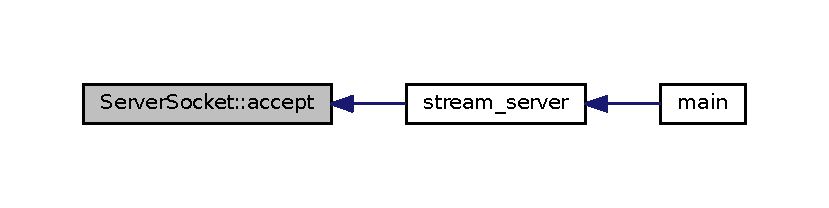
\includegraphics[width=350pt]{classServerSocket_a1d7054bc388f2d789d2124dd96939d90_icgraph}
\end{center}
\end{figure}




The documentation for this class was generated from the following files\+:\begin{DoxyCompactItemize}
\item 
include/\hyperlink{ServerSocket_8h}{Server\+Socket.\+h}\item 
src/\hyperlink{ServerSocket_8cpp}{Server\+Socket.\+cpp}\end{DoxyCompactItemize}

\hypertarget{classSocketFd}{\section{Socket\+Fd Class Reference}
\label{classSocketFd}\index{Socket\+Fd@{Socket\+Fd}}
}


Not initalizable Base\+Class for Socket\+File\+Descriptor.  




{\ttfamily \#include $<$Socket\+Fd.\+h$>$}



Inheritance diagram for Socket\+Fd\+:
\nopagebreak
\begin{figure}[H]
\begin{center}
\leavevmode
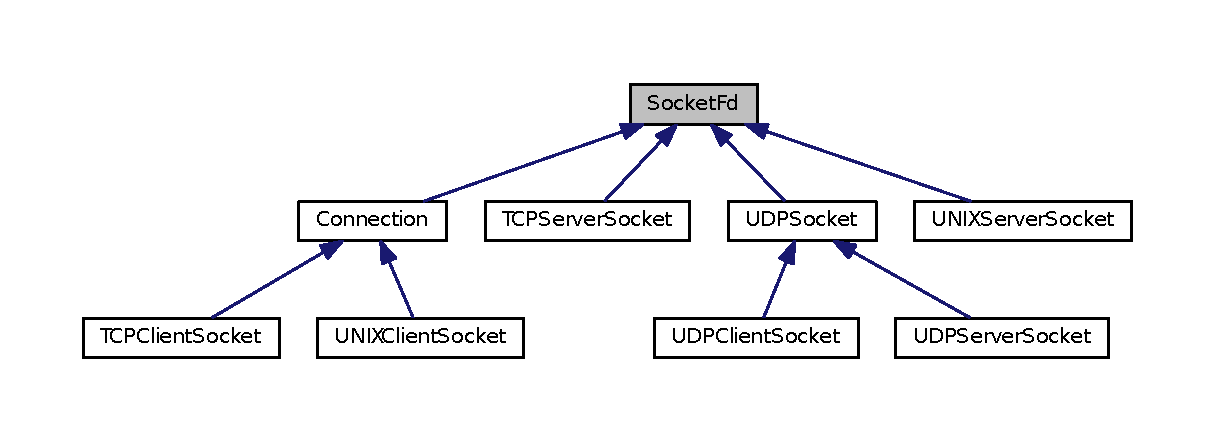
\includegraphics[width=350pt]{classSocketFd__inherit__graph}
\end{center}
\end{figure}
\subsection*{Public Member Functions}
\begin{DoxyCompactItemize}
\item 
virtual \hyperlink{classSocketFd_add3bcd5016a045da6ecccdfd4c97ee3f}{$\sim$\+Socket\+Fd} ()
\begin{DoxyCompactList}\small\item\em does nothing \end{DoxyCompactList}\item 
int \hyperlink{classSocketFd_a38ae432100f8df6e99e0145a793d4693}{set\+Non\+Blocking} ()
\begin{DoxyCompactList}\small\item\em make Sock\+Fd nonblocking \end{DoxyCompactList}\item 
int \hyperlink{classSocketFd_a0ebb54cefc45ab8e06472fb14e92c9e0}{set\+Blocking} ()
\begin{DoxyCompactList}\small\item\em make Sock\+Fd blocking \end{DoxyCompactList}\item 
int \hyperlink{classSocketFd_a9b3ed5d1b4e34195fd53ae8a627187aa}{set\+Timeout} (const unsigned sec, const unsigned msec=0)
\begin{DoxyCompactList}\small\item\em set Tiemout on Socket\+File\+Descriptor \end{DoxyCompactList}\end{DoxyCompactItemize}
\subsection*{Protected Member Functions}
\begin{DoxyCompactItemize}
\item 
\hyperlink{classSocketFd_a77eecdf99e10283d7bb3e0a7a0466a11}{Socket\+Fd} ()
\begin{DoxyCompactList}\small\item\em set Sock\+Fd to -\/1 \end{DoxyCompactList}\item 
void $\ast$ \hyperlink{classSocketFd_af0d8323eedd465a6a499df1129e19f7d}{get\+\_\+in\+\_\+addr} (sockaddr $\ast$)
\end{DoxyCompactItemize}
\subsection*{Protected Attributes}
\begin{DoxyCompactItemize}
\item 
pollfd \hyperlink{classSocketFd_a0636825d276c3525e0d8af969ce2d3b6}{ufds}
\end{DoxyCompactItemize}


\subsection{Detailed Description}
Not initalizable Base\+Class for Socket\+File\+Descriptor. 

Not initalizable Base\+Class for Socket\+File\+Descriptor. Provides means to setting timeout, non/blocking and getting addr of remote connection 

Definition at line 19 of file Socket\+Fd.\+h.



\subsection{Constructor \& Destructor Documentation}
\hypertarget{classSocketFd_a77eecdf99e10283d7bb3e0a7a0466a11}{\index{Socket\+Fd@{Socket\+Fd}!Socket\+Fd@{Socket\+Fd}}
\index{Socket\+Fd@{Socket\+Fd}!Socket\+Fd@{Socket\+Fd}}
\subsubsection[{Socket\+Fd}]{\setlength{\rightskip}{0pt plus 5cm}Socket\+Fd\+::\+Socket\+Fd (
\begin{DoxyParamCaption}
{}
\end{DoxyParamCaption}
)\hspace{0.3cm}{\ttfamily [protected]}}}\label{classSocketFd_a77eecdf99e10283d7bb3e0a7a0466a11}


set Sock\+Fd to -\/1 

set Sock\+Fd to -\/1 

Definition at line 3 of file Socket\+Fd.\+cpp.



References ufds.

\hypertarget{classSocketFd_add3bcd5016a045da6ecccdfd4c97ee3f}{\index{Socket\+Fd@{Socket\+Fd}!````~Socket\+Fd@{$\sim$\+Socket\+Fd}}
\index{````~Socket\+Fd@{$\sim$\+Socket\+Fd}!Socket\+Fd@{Socket\+Fd}}
\subsubsection[{$\sim$\+Socket\+Fd}]{\setlength{\rightskip}{0pt plus 5cm}Socket\+Fd\+::$\sim$\+Socket\+Fd (
\begin{DoxyParamCaption}
{}
\end{DoxyParamCaption}
)\hspace{0.3cm}{\ttfamily [virtual]}}}\label{classSocketFd_add3bcd5016a045da6ecccdfd4c97ee3f}


does nothing 

does nothing 

Definition at line 7 of file Socket\+Fd.\+cpp.



References ufds.



\subsection{Member Function Documentation}
\hypertarget{classSocketFd_af0d8323eedd465a6a499df1129e19f7d}{\index{Socket\+Fd@{Socket\+Fd}!get\+\_\+in\+\_\+addr@{get\+\_\+in\+\_\+addr}}
\index{get\+\_\+in\+\_\+addr@{get\+\_\+in\+\_\+addr}!Socket\+Fd@{Socket\+Fd}}
\subsubsection[{get\+\_\+in\+\_\+addr}]{\setlength{\rightskip}{0pt plus 5cm}void $\ast$ Socket\+Fd\+::get\+\_\+in\+\_\+addr (
\begin{DoxyParamCaption}
\item[{sockaddr $\ast$}]{sa}
\end{DoxyParamCaption}
)\hspace{0.3cm}{\ttfamily [protected]}}}\label{classSocketFd_af0d8323eedd465a6a499df1129e19f7d}
T\+O\+D\+O Add description 

Definition at line 26 of file Socket\+Fd.\+cpp.



Referenced by T\+C\+P\+Server\+Socket\+::accept(), and T\+C\+P\+Client\+Socket\+::\+T\+C\+P\+Client\+Socket().



Here is the caller graph for this function\+:
\nopagebreak
\begin{figure}[H]
\begin{center}
\leavevmode
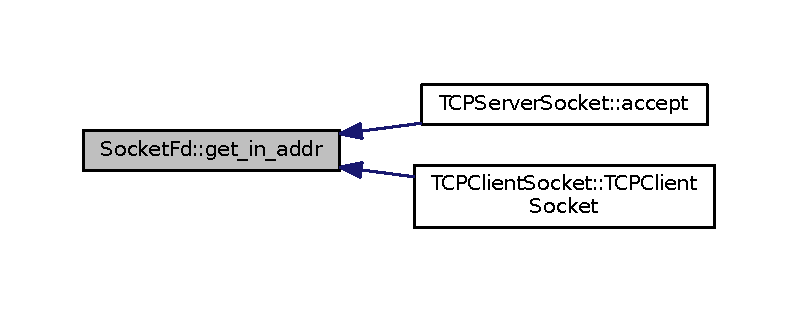
\includegraphics[width=350pt]{classSocketFd_af0d8323eedd465a6a499df1129e19f7d_icgraph}
\end{center}
\end{figure}


\hypertarget{classSocketFd_a0ebb54cefc45ab8e06472fb14e92c9e0}{\index{Socket\+Fd@{Socket\+Fd}!set\+Blocking@{set\+Blocking}}
\index{set\+Blocking@{set\+Blocking}!Socket\+Fd@{Socket\+Fd}}
\subsubsection[{set\+Blocking}]{\setlength{\rightskip}{0pt plus 5cm}int Socket\+Fd\+::set\+Blocking (
\begin{DoxyParamCaption}
{}
\end{DoxyParamCaption}
)}}\label{classSocketFd_a0ebb54cefc45ab8e06472fb14e92c9e0}


make Sock\+Fd blocking 

make Sock\+Fd blocking 

Definition at line 34 of file Socket\+Fd.\+cpp.



References ufds.

\hypertarget{classSocketFd_a38ae432100f8df6e99e0145a793d4693}{\index{Socket\+Fd@{Socket\+Fd}!set\+Non\+Blocking@{set\+Non\+Blocking}}
\index{set\+Non\+Blocking@{set\+Non\+Blocking}!Socket\+Fd@{Socket\+Fd}}
\subsubsection[{set\+Non\+Blocking}]{\setlength{\rightskip}{0pt plus 5cm}int Socket\+Fd\+::set\+Non\+Blocking (
\begin{DoxyParamCaption}
{}
\end{DoxyParamCaption}
)}}\label{classSocketFd_a38ae432100f8df6e99e0145a793d4693}


make Sock\+Fd nonblocking 

make Sock\+Fd nonblocking 

Definition at line 13 of file Socket\+Fd.\+cpp.



References ufds.

\hypertarget{classSocketFd_a9b3ed5d1b4e34195fd53ae8a627187aa}{\index{Socket\+Fd@{Socket\+Fd}!set\+Timeout@{set\+Timeout}}
\index{set\+Timeout@{set\+Timeout}!Socket\+Fd@{Socket\+Fd}}
\subsubsection[{set\+Timeout}]{\setlength{\rightskip}{0pt plus 5cm}int Socket\+Fd\+::set\+Timeout (
\begin{DoxyParamCaption}
\item[{const unsigned}]{sec, }
\item[{const unsigned}]{msec = {\ttfamily 0}}
\end{DoxyParamCaption}
)}}\label{classSocketFd_a9b3ed5d1b4e34195fd53ae8a627187aa}


set Tiemout on Socket\+File\+Descriptor 

set Tiemout on Socket\+File\+Descriptor 
\begin{DoxyParams}[1]{Parameters}
\mbox{\tt in}  & {\em sec} & Seconds to timeout \\
\hline
\mbox{\tt in}  & {\em msec} & Milliseconds to timeout \\
\hline
\end{DoxyParams}


Definition at line 47 of file Socket\+Fd.\+cpp.



References ufds.



Referenced by stream\+\_\+server().



Here is the caller graph for this function\+:
\nopagebreak
\begin{figure}[H]
\begin{center}
\leavevmode
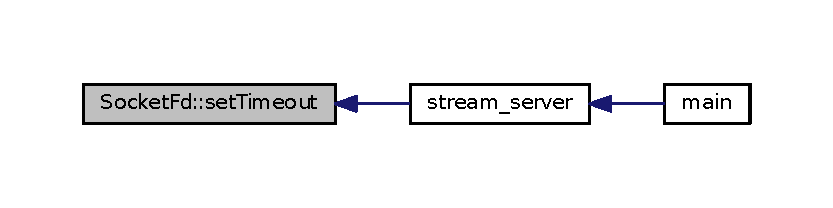
\includegraphics[width=350pt]{classSocketFd_a9b3ed5d1b4e34195fd53ae8a627187aa_icgraph}
\end{center}
\end{figure}




\subsection{Member Data Documentation}
\hypertarget{classSocketFd_a0636825d276c3525e0d8af969ce2d3b6}{\index{Socket\+Fd@{Socket\+Fd}!ufds@{ufds}}
\index{ufds@{ufds}!Socket\+Fd@{Socket\+Fd}}
\subsubsection[{ufds}]{\setlength{\rightskip}{0pt plus 5cm}pollfd Socket\+Fd\+::ufds\hspace{0.3cm}{\ttfamily [protected]}}}\label{classSocketFd_a0636825d276c3525e0d8af969ce2d3b6}
The Socket File Descriptor as a poll struct for Event Management 

Definition at line 26 of file Socket\+Fd.\+h.



Referenced by Connection\+::\+\_\+poll(), U\+N\+I\+X\+Server\+Socket\+::accept(), T\+C\+P\+Server\+Socket\+::accept(), Connection\+::\+Connection(), U\+D\+P\+Socket\+::recv(), U\+D\+P\+Socket\+::send(), set\+Blocking(), set\+Non\+Blocking(), set\+Timeout(), Socket\+Fd(), T\+C\+P\+Client\+Socket\+::\+T\+C\+P\+Client\+Socket(), T\+C\+P\+Server\+Socket\+::\+T\+C\+P\+Server\+Socket(), U\+D\+P\+Client\+Socket\+::\+U\+D\+P\+Client\+Socket(), U\+D\+P\+Server\+Socket\+::\+U\+D\+P\+Server\+Socket(), U\+N\+I\+X\+Client\+Socket\+::\+U\+N\+I\+X\+Client\+Socket(), U\+N\+I\+X\+Server\+Socket\+::\+U\+N\+I\+X\+Server\+Socket(), $\sim$\+Socket\+Fd(), and U\+D\+P\+Socket\+::$\sim$\+U\+D\+P\+Socket().



The documentation for this class was generated from the following files\+:\begin{DoxyCompactItemize}
\item 
include/\hyperlink{SocketFd_8h}{Socket\+Fd.\+h}\item 
src/\hyperlink{SocketFd_8cpp}{Socket\+Fd.\+cpp}\end{DoxyCompactItemize}

\hypertarget{classTCPClientSocket}{\section{T\+C\+P\+Client\+Socket Class Reference}
\label{classTCPClientSocket}\index{T\+C\+P\+Client\+Socket@{T\+C\+P\+Client\+Socket}}
}


{\ttfamily \#include $<$T\+C\+P\+Client\+Socket.\+h$>$}



Inheritance diagram for T\+C\+P\+Client\+Socket\+:
\nopagebreak
\begin{figure}[H]
\begin{center}
\leavevmode
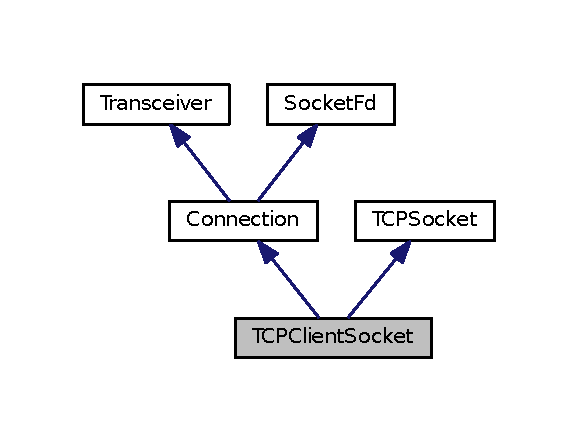
\includegraphics[width=278pt]{classTCPClientSocket__inherit__graph}
\end{center}
\end{figure}


Collaboration diagram for T\+C\+P\+Client\+Socket\+:
\nopagebreak
\begin{figure}[H]
\begin{center}
\leavevmode
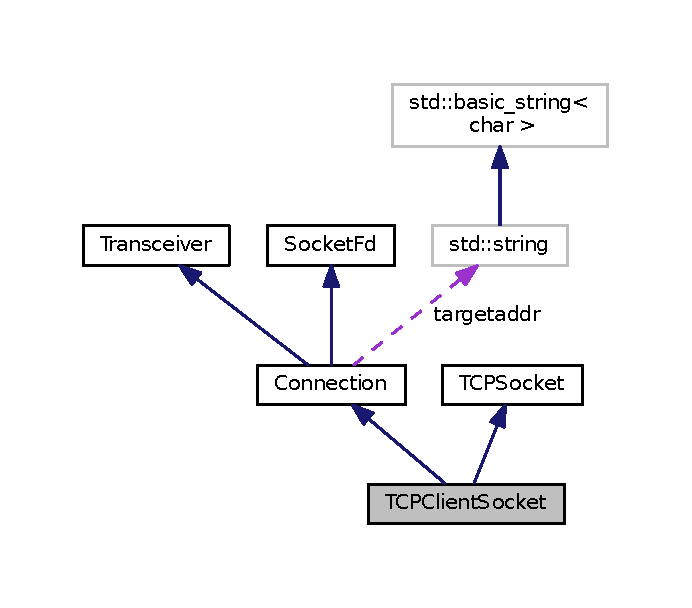
\includegraphics[width=332pt]{classTCPClientSocket__coll__graph}
\end{center}
\end{figure}
\subsection*{Public Member Functions}
\begin{DoxyCompactItemize}
\item 
\hyperlink{classTCPClientSocket_a3cdffa36ad33265b280c136ad597f9fd}{T\+C\+P\+Client\+Socket} (const char $\ast$, const unsigned)
\begin{DoxyCompactList}\small\item\em Construct a T\+C\+P connection. \end{DoxyCompactList}\item 
virtual \hyperlink{classTCPClientSocket_a9607474fe452def202cd23a6d7fecaae}{$\sim$\+T\+C\+P\+Client\+Socket} ()
\begin{DoxyCompactList}\small\item\em does nothing \end{DoxyCompactList}\end{DoxyCompactItemize}
\subsection*{Additional Inherited Members}


\subsection{Detailed Description}
A \hyperlink{classTCPClientSocket}{T\+C\+P\+Client\+Socket} establishes a connection on init Afterwards it can be used like a \hyperlink{classConnection}{Connection} Object. It directly provides \hyperlink{classConnection_a5466a66e569e81d891559686f2c7594b}{send()} and \hyperlink{classConnection_ab16b8a780c69303beec9b1f67fb596f3}{recv()} functions on init/connection error the Constructor throws a std\+::runtime\+\_\+error 

Definition at line 26 of file T\+C\+P\+Client\+Socket.\+h.



\subsection{Constructor \& Destructor Documentation}
\hypertarget{classTCPClientSocket_a3cdffa36ad33265b280c136ad597f9fd}{\index{T\+C\+P\+Client\+Socket@{T\+C\+P\+Client\+Socket}!T\+C\+P\+Client\+Socket@{T\+C\+P\+Client\+Socket}}
\index{T\+C\+P\+Client\+Socket@{T\+C\+P\+Client\+Socket}!T\+C\+P\+Client\+Socket@{T\+C\+P\+Client\+Socket}}
\subsubsection[{T\+C\+P\+Client\+Socket}]{\setlength{\rightskip}{0pt plus 5cm}T\+C\+P\+Client\+Socket\+::\+T\+C\+P\+Client\+Socket (
\begin{DoxyParamCaption}
\item[{const char $\ast$}]{host, }
\item[{const unsigned}]{iport}
\end{DoxyParamCaption}
)}}\label{classTCPClientSocket_a3cdffa36ad33265b280c136ad597f9fd}


Construct a T\+C\+P connection. 

Construct a T\+C\+P connection on error throws std\+::runtime\+\_\+error 

Definition at line 3 of file T\+C\+P\+Client\+Socket.\+cpp.



References Socket\+Fd\+::get\+\_\+in\+\_\+addr(), T\+C\+P\+Socket\+::hints, Connection\+::n, T\+C\+P\+Socket\+::p, T\+C\+P\+Socket\+::rv, T\+C\+P\+Socket\+::servinfo, Connection\+::targetaddr, and Socket\+Fd\+::ufds.



Here is the call graph for this function\+:
\nopagebreak
\begin{figure}[H]
\begin{center}
\leavevmode
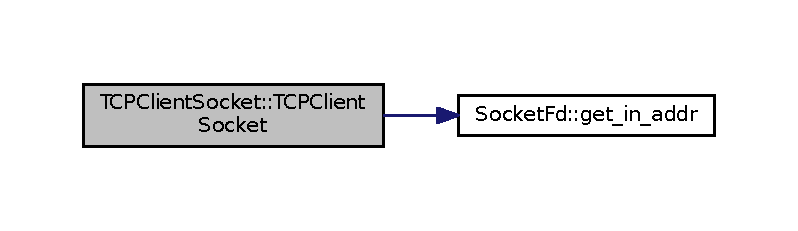
\includegraphics[width=350pt]{classTCPClientSocket_a3cdffa36ad33265b280c136ad597f9fd_cgraph}
\end{center}
\end{figure}


\hypertarget{classTCPClientSocket_a9607474fe452def202cd23a6d7fecaae}{\index{T\+C\+P\+Client\+Socket@{T\+C\+P\+Client\+Socket}!````~T\+C\+P\+Client\+Socket@{$\sim$\+T\+C\+P\+Client\+Socket}}
\index{````~T\+C\+P\+Client\+Socket@{$\sim$\+T\+C\+P\+Client\+Socket}!T\+C\+P\+Client\+Socket@{T\+C\+P\+Client\+Socket}}
\subsubsection[{$\sim$\+T\+C\+P\+Client\+Socket}]{\setlength{\rightskip}{0pt plus 5cm}T\+C\+P\+Client\+Socket\+::$\sim$\+T\+C\+P\+Client\+Socket (
\begin{DoxyParamCaption}
{}
\end{DoxyParamCaption}
)\hspace{0.3cm}{\ttfamily [virtual]}}}\label{classTCPClientSocket_a9607474fe452def202cd23a6d7fecaae}


does nothing 

does nothing 

Definition at line 56 of file T\+C\+P\+Client\+Socket.\+cpp.



The documentation for this class was generated from the following files\+:\begin{DoxyCompactItemize}
\item 
include/\hyperlink{TCPClientSocket_8h}{T\+C\+P\+Client\+Socket.\+h}\item 
src/\hyperlink{TCPClientSocket_8cpp}{T\+C\+P\+Client\+Socket.\+cpp}\end{DoxyCompactItemize}

\hypertarget{classTCPServerSocket}{\section{T\+C\+P\+Server\+Socket Class Reference}
\label{classTCPServerSocket}\index{T\+C\+P\+Server\+Socket@{T\+C\+P\+Server\+Socket}}
}


{\ttfamily \#include $<$T\+C\+P\+Server\+Socket.\+h$>$}



Inheritance diagram for T\+C\+P\+Server\+Socket\+:
\nopagebreak
\begin{figure}[H]
\begin{center}
\leavevmode
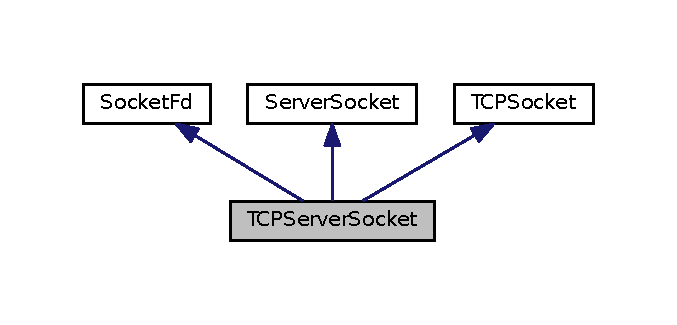
\includegraphics[width=325pt]{classTCPServerSocket__inherit__graph}
\end{center}
\end{figure}


Collaboration diagram for T\+C\+P\+Server\+Socket\+:
\nopagebreak
\begin{figure}[H]
\begin{center}
\leavevmode
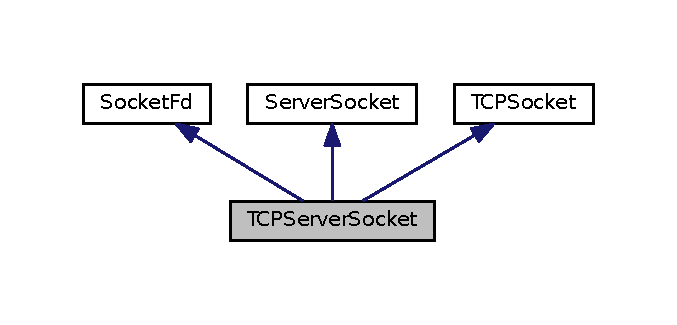
\includegraphics[width=325pt]{classTCPServerSocket__coll__graph}
\end{center}
\end{figure}
\subsection*{Public Member Functions}
\begin{DoxyCompactItemize}
\item 
\hyperlink{classTCPServerSocket_a2a54360b0df69bbbbd088bb60ba1c93a}{T\+C\+P\+Server\+Socket} (const unsigned)
\begin{DoxyCompactList}\small\item\em construct a listening Socket \end{DoxyCompactList}\item 
virtual \hyperlink{classTCPServerSocket_ac585f0ee1919733ec028dadf9c204ddf}{$\sim$\+T\+C\+P\+Server\+Socket} ()
\begin{DoxyCompactList}\small\item\em does nothing \end{DoxyCompactList}\item 
\hyperlink{classConnection}{Connection} $\ast$ \hyperlink{classTCPServerSocket_a0c169a85290095c3c58b9fae38a1a1d0}{accept} ()
\begin{DoxyCompactList}\small\item\em accept incoming tcp connections \end{DoxyCompactList}\end{DoxyCompactItemize}
\subsection*{Additional Inherited Members}


\subsection{Detailed Description}
A \hyperlink{classTCPServerSocket}{T\+C\+P\+Server\+Socket} provides a means for T\+C\+P Clients to be Accepted with the \hyperlink{classTCPServerSocket_a0c169a85290095c3c58b9fae38a1a1d0}{accept()} methode it provides if the construction failes and the Listen Port can not be accessed the constructor will throw a runtime\+\_\+error 

Definition at line 26 of file T\+C\+P\+Server\+Socket.\+h.



\subsection{Constructor \& Destructor Documentation}
\hypertarget{classTCPServerSocket_a2a54360b0df69bbbbd088bb60ba1c93a}{\index{T\+C\+P\+Server\+Socket@{T\+C\+P\+Server\+Socket}!T\+C\+P\+Server\+Socket@{T\+C\+P\+Server\+Socket}}
\index{T\+C\+P\+Server\+Socket@{T\+C\+P\+Server\+Socket}!T\+C\+P\+Server\+Socket@{T\+C\+P\+Server\+Socket}}
\subsubsection[{T\+C\+P\+Server\+Socket}]{\setlength{\rightskip}{0pt plus 5cm}T\+C\+P\+Server\+Socket\+::\+T\+C\+P\+Server\+Socket (
\begin{DoxyParamCaption}
\item[{const unsigned}]{iport}
\end{DoxyParamCaption}
)}}\label{classTCPServerSocket_a2a54360b0df69bbbbd088bb60ba1c93a}


construct a listening Socket 

constructs a listening Socket will throw runtime\+\_\+error if something goes wrong 

Definition at line 3 of file T\+C\+P\+Server\+Socket.\+cpp.



References T\+C\+P\+Socket\+::hints, T\+C\+P\+Socket\+::p, T\+C\+P\+Socket\+::rv, T\+C\+P\+Socket\+::servinfo, and Socket\+Fd\+::ufds.

\hypertarget{classTCPServerSocket_ac585f0ee1919733ec028dadf9c204ddf}{\index{T\+C\+P\+Server\+Socket@{T\+C\+P\+Server\+Socket}!````~T\+C\+P\+Server\+Socket@{$\sim$\+T\+C\+P\+Server\+Socket}}
\index{````~T\+C\+P\+Server\+Socket@{$\sim$\+T\+C\+P\+Server\+Socket}!T\+C\+P\+Server\+Socket@{T\+C\+P\+Server\+Socket}}
\subsubsection[{$\sim$\+T\+C\+P\+Server\+Socket}]{\setlength{\rightskip}{0pt plus 5cm}T\+C\+P\+Server\+Socket\+::$\sim$\+T\+C\+P\+Server\+Socket (
\begin{DoxyParamCaption}
{}
\end{DoxyParamCaption}
)\hspace{0.3cm}{\ttfamily [virtual]}}}\label{classTCPServerSocket_ac585f0ee1919733ec028dadf9c204ddf}


does nothing 

does nothing 

Definition at line 64 of file T\+C\+P\+Server\+Socket.\+cpp.



\subsection{Member Function Documentation}
\hypertarget{classTCPServerSocket_a0c169a85290095c3c58b9fae38a1a1d0}{\index{T\+C\+P\+Server\+Socket@{T\+C\+P\+Server\+Socket}!accept@{accept}}
\index{accept@{accept}!T\+C\+P\+Server\+Socket@{T\+C\+P\+Server\+Socket}}
\subsubsection[{accept}]{\setlength{\rightskip}{0pt plus 5cm}{\bf Connection} $\ast$ T\+C\+P\+Server\+Socket\+::accept (
\begin{DoxyParamCaption}
{}
\end{DoxyParamCaption}
)\hspace{0.3cm}{\ttfamily [virtual]}}}\label{classTCPServerSocket_a0c169a85290095c3c58b9fae38a1a1d0}


accept incoming tcp connections 

accept incoming tcp connections 

Implements \hyperlink{classServerSocket_a1d7054bc388f2d789d2124dd96939d90}{Server\+Socket}.



Definition at line 67 of file T\+C\+P\+Server\+Socket.\+cpp.



References Socket\+Fd\+::get\+\_\+in\+\_\+addr(), T\+C\+P\+Socket\+::slen, T\+C\+P\+Socket\+::their\+\_\+addr, and Socket\+Fd\+::ufds.



Here is the call graph for this function\+:
\nopagebreak
\begin{figure}[H]
\begin{center}
\leavevmode
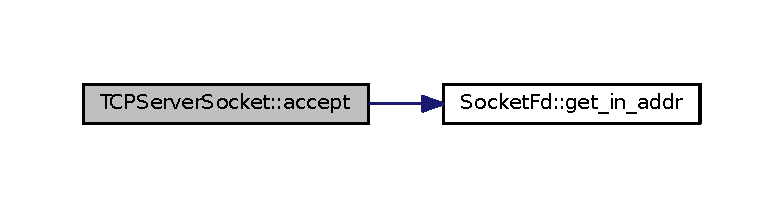
\includegraphics[width=350pt]{classTCPServerSocket_a0c169a85290095c3c58b9fae38a1a1d0_cgraph}
\end{center}
\end{figure}




The documentation for this class was generated from the following files\+:\begin{DoxyCompactItemize}
\item 
include/\hyperlink{TCPServerSocket_8h}{T\+C\+P\+Server\+Socket.\+h}\item 
src/\hyperlink{TCPServerSocket_8cpp}{T\+C\+P\+Server\+Socket.\+cpp}\end{DoxyCompactItemize}

\hypertarget{classTCPSocket}{\section{T\+C\+P\+Socket Class Reference}
\label{classTCPSocket}\index{T\+C\+P\+Socket@{T\+C\+P\+Socket}}
}


{\ttfamily \#include $<$T\+C\+P\+Socket.\+h$>$}



Inheritance diagram for T\+C\+P\+Socket\+:
\nopagebreak
\begin{figure}[H]
\begin{center}
\leavevmode
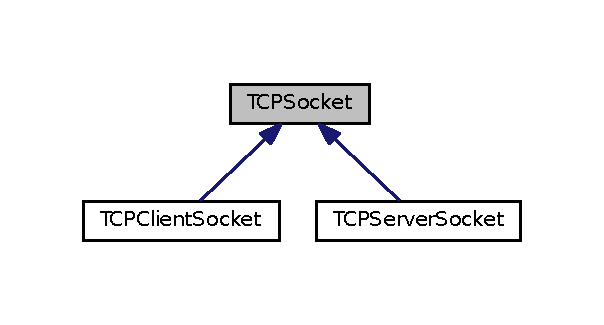
\includegraphics[width=290pt]{classTCPSocket__inherit__graph}
\end{center}
\end{figure}
\subsection*{Public Member Functions}
\begin{DoxyCompactItemize}
\item 
virtual \hyperlink{classTCPSocket_af357e6923a0f8adbbb8e46fab4523991}{$\sim$\+T\+C\+P\+Socket} ()
\end{DoxyCompactItemize}
\subsection*{Protected Member Functions}
\begin{DoxyCompactItemize}
\item 
\hyperlink{classTCPSocket_a7a50427a401d1a6f3209d51818bad901}{T\+C\+P\+Socket} ()
\end{DoxyCompactItemize}
\subsection*{Protected Attributes}
\begin{DoxyCompactItemize}
\item 
int \hyperlink{classTCPSocket_a2f6471b799685ee580a9cfa5d94ac3a7}{rv}
\item 
socklen\+\_\+t \hyperlink{classTCPSocket_a9613e3899f39278d0de6fab677bb1edc}{slen}
\item 
addrinfo \hyperlink{classTCPSocket_a76a561d3c5594dd8bc7f57a10add34b8}{hints}
\item 
addrinfo $\ast$ \hyperlink{classTCPSocket_a79ce3d1a12b7371a6838dad34d0e8cf3}{servinfo}
\item 
addrinfo $\ast$ \hyperlink{classTCPSocket_a772833fd0273c3e0bcb1888084d38799}{p}
\item 
sockaddr\+\_\+storage \hyperlink{classTCPSocket_a54b0073827ac57bbb4ee6c371791db0f}{their\+\_\+addr}
\end{DoxyCompactItemize}


\subsection{Detailed Description}
Non constructable Base\+Class for T\+C\+P Sockets just because they share some structs This is purely for internal use 

Definition at line 15 of file T\+C\+P\+Socket.\+h.



\subsection{Constructor \& Destructor Documentation}
\hypertarget{classTCPSocket_a7a50427a401d1a6f3209d51818bad901}{\index{T\+C\+P\+Socket@{T\+C\+P\+Socket}!T\+C\+P\+Socket@{T\+C\+P\+Socket}}
\index{T\+C\+P\+Socket@{T\+C\+P\+Socket}!T\+C\+P\+Socket@{T\+C\+P\+Socket}}
\subsubsection[{T\+C\+P\+Socket}]{\setlength{\rightskip}{0pt plus 5cm}T\+C\+P\+Socket\+::\+T\+C\+P\+Socket (
\begin{DoxyParamCaption}
{}
\end{DoxyParamCaption}
)\hspace{0.3cm}{\ttfamily [protected]}}}\label{classTCPSocket_a7a50427a401d1a6f3209d51818bad901}


Definition at line 6 of file T\+C\+P\+Socket.\+cpp.



References p, rv, servinfo, and slen.

\hypertarget{classTCPSocket_af357e6923a0f8adbbb8e46fab4523991}{\index{T\+C\+P\+Socket@{T\+C\+P\+Socket}!````~T\+C\+P\+Socket@{$\sim$\+T\+C\+P\+Socket}}
\index{````~T\+C\+P\+Socket@{$\sim$\+T\+C\+P\+Socket}!T\+C\+P\+Socket@{T\+C\+P\+Socket}}
\subsubsection[{$\sim$\+T\+C\+P\+Socket}]{\setlength{\rightskip}{0pt plus 5cm}T\+C\+P\+Socket\+::$\sim$\+T\+C\+P\+Socket (
\begin{DoxyParamCaption}
{}
\end{DoxyParamCaption}
)\hspace{0.3cm}{\ttfamily [virtual]}}}\label{classTCPSocket_af357e6923a0f8adbbb8e46fab4523991}


Definition at line 3 of file T\+C\+P\+Socket.\+cpp.



\subsection{Member Data Documentation}
\hypertarget{classTCPSocket_a76a561d3c5594dd8bc7f57a10add34b8}{\index{T\+C\+P\+Socket@{T\+C\+P\+Socket}!hints@{hints}}
\index{hints@{hints}!T\+C\+P\+Socket@{T\+C\+P\+Socket}}
\subsubsection[{hints}]{\setlength{\rightskip}{0pt plus 5cm}addrinfo T\+C\+P\+Socket\+::hints\hspace{0.3cm}{\ttfamily [protected]}}}\label{classTCPSocket_a76a561d3c5594dd8bc7f57a10add34b8}


Definition at line 19 of file T\+C\+P\+Socket.\+h.



Referenced by T\+C\+P\+Client\+Socket\+::\+T\+C\+P\+Client\+Socket(), and T\+C\+P\+Server\+Socket\+::\+T\+C\+P\+Server\+Socket().

\hypertarget{classTCPSocket_a772833fd0273c3e0bcb1888084d38799}{\index{T\+C\+P\+Socket@{T\+C\+P\+Socket}!p@{p}}
\index{p@{p}!T\+C\+P\+Socket@{T\+C\+P\+Socket}}
\subsubsection[{p}]{\setlength{\rightskip}{0pt plus 5cm}addrinfo $\ast$ T\+C\+P\+Socket\+::p\hspace{0.3cm}{\ttfamily [protected]}}}\label{classTCPSocket_a772833fd0273c3e0bcb1888084d38799}


Definition at line 19 of file T\+C\+P\+Socket.\+h.



Referenced by T\+C\+P\+Client\+Socket\+::\+T\+C\+P\+Client\+Socket(), T\+C\+P\+Server\+Socket\+::\+T\+C\+P\+Server\+Socket(), and T\+C\+P\+Socket().

\hypertarget{classTCPSocket_a2f6471b799685ee580a9cfa5d94ac3a7}{\index{T\+C\+P\+Socket@{T\+C\+P\+Socket}!rv@{rv}}
\index{rv@{rv}!T\+C\+P\+Socket@{T\+C\+P\+Socket}}
\subsubsection[{rv}]{\setlength{\rightskip}{0pt plus 5cm}int T\+C\+P\+Socket\+::rv\hspace{0.3cm}{\ttfamily [protected]}}}\label{classTCPSocket_a2f6471b799685ee580a9cfa5d94ac3a7}


Definition at line 17 of file T\+C\+P\+Socket.\+h.



Referenced by T\+C\+P\+Client\+Socket\+::\+T\+C\+P\+Client\+Socket(), T\+C\+P\+Server\+Socket\+::\+T\+C\+P\+Server\+Socket(), and T\+C\+P\+Socket().

\hypertarget{classTCPSocket_a79ce3d1a12b7371a6838dad34d0e8cf3}{\index{T\+C\+P\+Socket@{T\+C\+P\+Socket}!servinfo@{servinfo}}
\index{servinfo@{servinfo}!T\+C\+P\+Socket@{T\+C\+P\+Socket}}
\subsubsection[{servinfo}]{\setlength{\rightskip}{0pt plus 5cm}addrinfo $\ast$ T\+C\+P\+Socket\+::servinfo\hspace{0.3cm}{\ttfamily [protected]}}}\label{classTCPSocket_a79ce3d1a12b7371a6838dad34d0e8cf3}


Definition at line 19 of file T\+C\+P\+Socket.\+h.



Referenced by T\+C\+P\+Client\+Socket\+::\+T\+C\+P\+Client\+Socket(), T\+C\+P\+Server\+Socket\+::\+T\+C\+P\+Server\+Socket(), and T\+C\+P\+Socket().

\hypertarget{classTCPSocket_a9613e3899f39278d0de6fab677bb1edc}{\index{T\+C\+P\+Socket@{T\+C\+P\+Socket}!slen@{slen}}
\index{slen@{slen}!T\+C\+P\+Socket@{T\+C\+P\+Socket}}
\subsubsection[{slen}]{\setlength{\rightskip}{0pt plus 5cm}socklen\+\_\+t T\+C\+P\+Socket\+::slen\hspace{0.3cm}{\ttfamily [protected]}}}\label{classTCPSocket_a9613e3899f39278d0de6fab677bb1edc}


Definition at line 18 of file T\+C\+P\+Socket.\+h.



Referenced by T\+C\+P\+Server\+Socket\+::accept(), and T\+C\+P\+Socket().

\hypertarget{classTCPSocket_a54b0073827ac57bbb4ee6c371791db0f}{\index{T\+C\+P\+Socket@{T\+C\+P\+Socket}!their\+\_\+addr@{their\+\_\+addr}}
\index{their\+\_\+addr@{their\+\_\+addr}!T\+C\+P\+Socket@{T\+C\+P\+Socket}}
\subsubsection[{their\+\_\+addr}]{\setlength{\rightskip}{0pt plus 5cm}sockaddr\+\_\+storage T\+C\+P\+Socket\+::their\+\_\+addr\hspace{0.3cm}{\ttfamily [protected]}}}\label{classTCPSocket_a54b0073827ac57bbb4ee6c371791db0f}


Definition at line 20 of file T\+C\+P\+Socket.\+h.



Referenced by T\+C\+P\+Server\+Socket\+::accept().



The documentation for this class was generated from the following files\+:\begin{DoxyCompactItemize}
\item 
include/\hyperlink{TCPSocket_8h}{T\+C\+P\+Socket.\+h}\item 
src/\hyperlink{TCPSocket_8cpp}{T\+C\+P\+Socket.\+cpp}\end{DoxyCompactItemize}

\hypertarget{classTransceiver}{\section{Transceiver Class Reference}
\label{classTransceiver}\index{Transceiver@{Transceiver}}
}


{\ttfamily \#include $<$Transceiver.\+h$>$}



Inheritance diagram for Transceiver\+:
\nopagebreak
\begin{figure}[H]
\begin{center}
\leavevmode
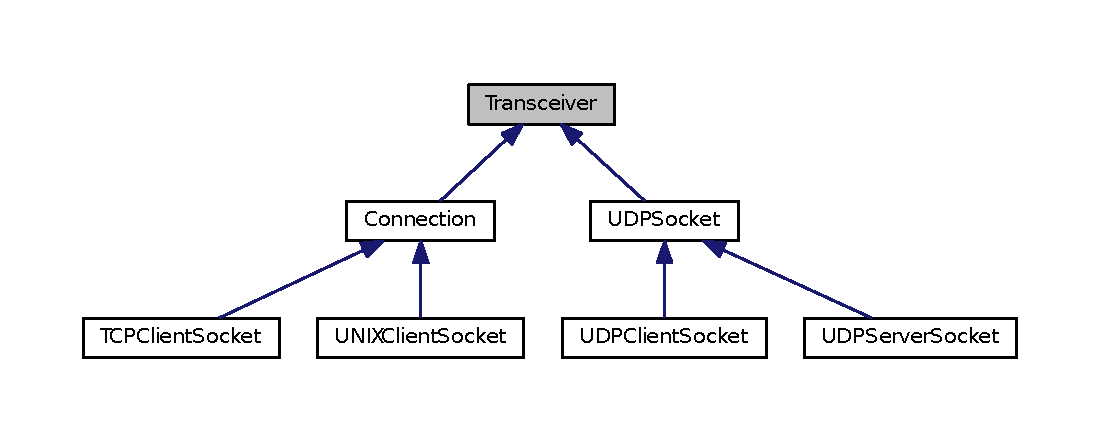
\includegraphics[width=350pt]{classTransceiver__inherit__graph}
\end{center}
\end{figure}
\subsection*{Public Member Functions}
\begin{DoxyCompactItemize}
\item 
virtual \hyperlink{classTransceiver_a09118fef519a75434a3f42ab7d506c74}{$\sim$\+Transceiver} ()
\item 
virtual int \hyperlink{classTransceiver_aa54935e0032d9ab6c531024e001ae19d}{send} (const char $\ast$, const unsigned, const int=0)=0
\item 
virtual int \hyperlink{classTransceiver_aef7153a423766522f4f82c1300157048}{recv} (char $\ast$, const unsigned, const int=0)=0
\end{DoxyCompactItemize}
\subsection*{Protected Member Functions}
\begin{DoxyCompactItemize}
\item 
\hyperlink{classTransceiver_a8a846d40a2108ebe79003e231d9968e3}{Transceiver} ()
\end{DoxyCompactItemize}


\subsection{Detailed Description}
virtual Base\+Class for Classes that should provide a \hyperlink{classTransceiver_aa54935e0032d9ab6c531024e001ae19d}{send()} and \hyperlink{classTransceiver_aef7153a423766522f4f82c1300157048}{recv()} method 

Definition at line 7 of file Transceiver.\+h.



\subsection{Constructor \& Destructor Documentation}
\hypertarget{classTransceiver_a8a846d40a2108ebe79003e231d9968e3}{\index{Transceiver@{Transceiver}!Transceiver@{Transceiver}}
\index{Transceiver@{Transceiver}!Transceiver@{Transceiver}}
\subsubsection[{Transceiver}]{\setlength{\rightskip}{0pt plus 5cm}Transceiver\+::\+Transceiver (
\begin{DoxyParamCaption}
{}
\end{DoxyParamCaption}
)\hspace{0.3cm}{\ttfamily [protected]}}}\label{classTransceiver_a8a846d40a2108ebe79003e231d9968e3}


Definition at line 3 of file Transceiver.\+cpp.

\hypertarget{classTransceiver_a09118fef519a75434a3f42ab7d506c74}{\index{Transceiver@{Transceiver}!````~Transceiver@{$\sim$\+Transceiver}}
\index{````~Transceiver@{$\sim$\+Transceiver}!Transceiver@{Transceiver}}
\subsubsection[{$\sim$\+Transceiver}]{\setlength{\rightskip}{0pt plus 5cm}Transceiver\+::$\sim$\+Transceiver (
\begin{DoxyParamCaption}
{}
\end{DoxyParamCaption}
)\hspace{0.3cm}{\ttfamily [virtual]}}}\label{classTransceiver_a09118fef519a75434a3f42ab7d506c74}


Definition at line 6 of file Transceiver.\+cpp.



\subsection{Member Function Documentation}
\hypertarget{classTransceiver_aef7153a423766522f4f82c1300157048}{\index{Transceiver@{Transceiver}!recv@{recv}}
\index{recv@{recv}!Transceiver@{Transceiver}}
\subsubsection[{recv}]{\setlength{\rightskip}{0pt plus 5cm}virtual int Transceiver\+::recv (
\begin{DoxyParamCaption}
\item[{char $\ast$}]{, }
\item[{const unsigned}]{, }
\item[{const int}]{ = {\ttfamily 0}}
\end{DoxyParamCaption}
)\hspace{0.3cm}{\ttfamily [pure virtual]}}}\label{classTransceiver_aef7153a423766522f4f82c1300157048}


Implemented in \hyperlink{classUDPSocket_a712f913657579110edb1f6befbc4a279}{U\+D\+P\+Socket}, and \hyperlink{classConnection_ab16b8a780c69303beec9b1f67fb596f3}{Connection}.

\hypertarget{classTransceiver_aa54935e0032d9ab6c531024e001ae19d}{\index{Transceiver@{Transceiver}!send@{send}}
\index{send@{send}!Transceiver@{Transceiver}}
\subsubsection[{send}]{\setlength{\rightskip}{0pt plus 5cm}virtual int Transceiver\+::send (
\begin{DoxyParamCaption}
\item[{const char $\ast$}]{, }
\item[{const unsigned}]{, }
\item[{const int}]{ = {\ttfamily 0}}
\end{DoxyParamCaption}
)\hspace{0.3cm}{\ttfamily [pure virtual]}}}\label{classTransceiver_aa54935e0032d9ab6c531024e001ae19d}


Implemented in \hyperlink{classUDPSocket_a1c6cf2ad03b21ad00029d5f51fde43f5}{U\+D\+P\+Socket}, and \hyperlink{classConnection_a5466a66e569e81d891559686f2c7594b}{Connection}.



The documentation for this class was generated from the following files\+:\begin{DoxyCompactItemize}
\item 
include/\hyperlink{Transceiver_8h}{Transceiver.\+h}\item 
src/\hyperlink{Transceiver_8cpp}{Transceiver.\+cpp}\end{DoxyCompactItemize}

\hypertarget{classUDPClientSocket}{\section{U\+D\+P\+Client\+Socket Class Reference}
\label{classUDPClientSocket}\index{U\+D\+P\+Client\+Socket@{U\+D\+P\+Client\+Socket}}
}


{\ttfamily \#include $<$U\+D\+P\+Client\+Socket.\+h$>$}



Inheritance diagram for U\+D\+P\+Client\+Socket\+:
\nopagebreak
\begin{figure}[H]
\begin{center}
\leavevmode
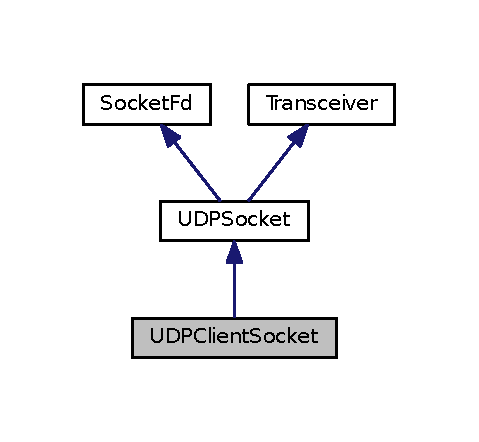
\includegraphics[width=230pt]{classUDPClientSocket__inherit__graph}
\end{center}
\end{figure}


Collaboration diagram for U\+D\+P\+Client\+Socket\+:
\nopagebreak
\begin{figure}[H]
\begin{center}
\leavevmode
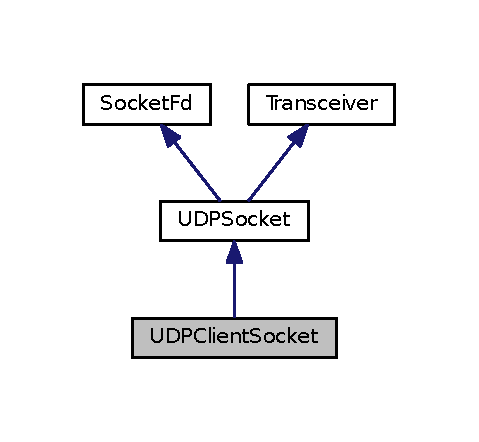
\includegraphics[width=230pt]{classUDPClientSocket__coll__graph}
\end{center}
\end{figure}
\subsection*{Public Member Functions}
\begin{DoxyCompactItemize}
\item 
\hyperlink{classUDPClientSocket_a948d4d68b8cfb63efbed66556b934101}{U\+D\+P\+Client\+Socket} (const char $\ast$addr, const unsigned int port)
\begin{DoxyCompactList}\small\item\em construct \hyperlink{classUDPClientSocket}{U\+D\+P\+Client\+Socket} \end{DoxyCompactList}\item 
virtual \hyperlink{classUDPClientSocket_a055f430e2111d669cef3af07cec07b56}{$\sim$\+U\+D\+P\+Client\+Socket} ()
\begin{DoxyCompactList}\small\item\em does nothing \end{DoxyCompactList}\end{DoxyCompactItemize}
\subsection*{Additional Inherited Members}


\subsection{Detailed Description}
A \hyperlink{classUDPClientSocket}{U\+D\+P\+Client\+Socket} is read to \hyperlink{classUDPSocket_a1c6cf2ad03b21ad00029d5f51fde43f5}{send()} and \hyperlink{classUDPSocket_a712f913657579110edb1f6befbc4a279}{recv()} data after construction if construction failes a runtime\+\_\+error is thrown Base\+Cöass is \hyperlink{classConnection}{Connection} 

Definition at line 21 of file U\+D\+P\+Client\+Socket.\+h.



\subsection{Constructor \& Destructor Documentation}
\hypertarget{classUDPClientSocket_a948d4d68b8cfb63efbed66556b934101}{\index{U\+D\+P\+Client\+Socket@{U\+D\+P\+Client\+Socket}!U\+D\+P\+Client\+Socket@{U\+D\+P\+Client\+Socket}}
\index{U\+D\+P\+Client\+Socket@{U\+D\+P\+Client\+Socket}!U\+D\+P\+Client\+Socket@{U\+D\+P\+Client\+Socket}}
\subsubsection[{U\+D\+P\+Client\+Socket}]{\setlength{\rightskip}{0pt plus 5cm}U\+D\+P\+Client\+Socket\+::\+U\+D\+P\+Client\+Socket (
\begin{DoxyParamCaption}
\item[{const char $\ast$}]{addr, }
\item[{const unsigned int}]{port}
\end{DoxyParamCaption}
)}}\label{classUDPClientSocket_a948d4d68b8cfb63efbed66556b934101}


construct \hyperlink{classUDPClientSocket}{U\+D\+P\+Client\+Socket} 

construct \hyperlink{classUDPClientSocket}{U\+D\+P\+Client\+Socket} 
\begin{DoxyParams}[1]{Parameters}
\mbox{\tt in}  & {\em addr} & The Address of the host \\
\hline
\mbox{\tt in}  & {\em port} & The Port the host is listening on \\
\hline
\end{DoxyParams}


Definition at line 3 of file U\+D\+P\+Client\+Socket.\+cpp.



References U\+D\+P\+Socket\+::hints, U\+D\+P\+Socket\+::p, U\+D\+P\+Socket\+::rv, U\+D\+P\+Socket\+::servinfo, and Socket\+Fd\+::ufds.

\hypertarget{classUDPClientSocket_a055f430e2111d669cef3af07cec07b56}{\index{U\+D\+P\+Client\+Socket@{U\+D\+P\+Client\+Socket}!````~U\+D\+P\+Client\+Socket@{$\sim$\+U\+D\+P\+Client\+Socket}}
\index{````~U\+D\+P\+Client\+Socket@{$\sim$\+U\+D\+P\+Client\+Socket}!U\+D\+P\+Client\+Socket@{U\+D\+P\+Client\+Socket}}
\subsubsection[{$\sim$\+U\+D\+P\+Client\+Socket}]{\setlength{\rightskip}{0pt plus 5cm}U\+D\+P\+Client\+Socket\+::$\sim$\+U\+D\+P\+Client\+Socket (
\begin{DoxyParamCaption}
{}
\end{DoxyParamCaption}
)\hspace{0.3cm}{\ttfamily [virtual]}}}\label{classUDPClientSocket_a055f430e2111d669cef3af07cec07b56}


does nothing 

does nothing 

Definition at line 37 of file U\+D\+P\+Client\+Socket.\+cpp.



The documentation for this class was generated from the following files\+:\begin{DoxyCompactItemize}
\item 
include/\hyperlink{UDPClientSocket_8h}{U\+D\+P\+Client\+Socket.\+h}\item 
src/\hyperlink{UDPClientSocket_8cpp}{U\+D\+P\+Client\+Socket.\+cpp}\end{DoxyCompactItemize}

\hypertarget{classUDPServerSocket}{\section{U\+D\+P\+Server\+Socket Class Reference}
\label{classUDPServerSocket}\index{U\+D\+P\+Server\+Socket@{U\+D\+P\+Server\+Socket}}
}


{\ttfamily \#include $<$U\+D\+P\+Server\+Socket.\+h$>$}



Inheritance diagram for U\+D\+P\+Server\+Socket\+:
\nopagebreak
\begin{figure}[H]
\begin{center}
\leavevmode
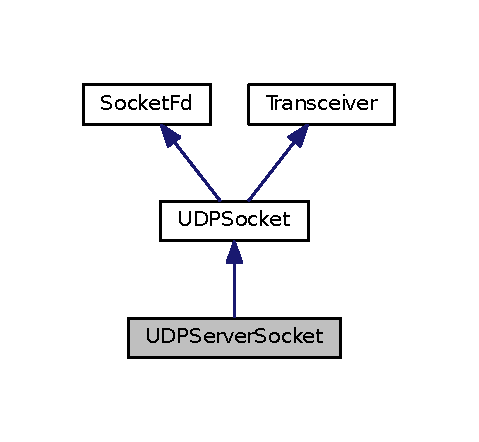
\includegraphics[width=230pt]{classUDPServerSocket__inherit__graph}
\end{center}
\end{figure}


Collaboration diagram for U\+D\+P\+Server\+Socket\+:
\nopagebreak
\begin{figure}[H]
\begin{center}
\leavevmode
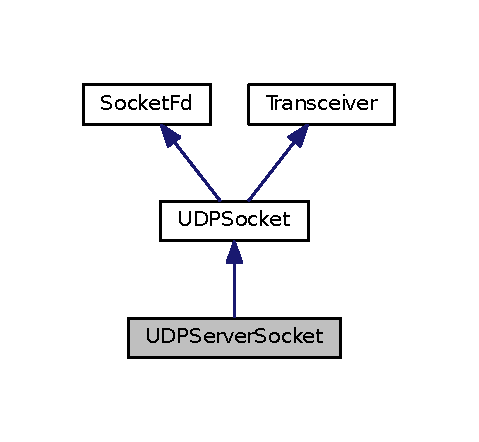
\includegraphics[width=230pt]{classUDPServerSocket__coll__graph}
\end{center}
\end{figure}
\subsection*{Public Member Functions}
\begin{DoxyCompactItemize}
\item 
\hyperlink{classUDPServerSocket_adb12550f85fb5d61aad8dd4e87a5e9d7}{U\+D\+P\+Server\+Socket} (const unsigned)
\begin{DoxyCompactList}\small\item\em creates U\+D\+P listening Socket \end{DoxyCompactList}\item 
virtual \hyperlink{classUDPServerSocket_a3725e9f63fd753989c66f2ece4cf0370}{$\sim$\+U\+D\+P\+Server\+Socket} ()
\begin{DoxyCompactList}\small\item\em does nothing \end{DoxyCompactList}\end{DoxyCompactItemize}
\subsection*{Additional Inherited Members}


\subsection{Detailed Description}
A \hyperlink{classUDPServerSocket}{U\+D\+P\+Server\+Socket} is a U\+D\+P listening Socket provides \hyperlink{classUDPSocket_a1c6cf2ad03b21ad00029d5f51fde43f5}{send()} and \hyperlink{classUDPSocket_a712f913657579110edb1f6befbc4a279}{recv()} methods after construction Base\+Class is a \hyperlink{classConnection}{Connection} Object throws runtime\+\_\+error on construction failure 

Definition at line 23 of file U\+D\+P\+Server\+Socket.\+h.



\subsection{Constructor \& Destructor Documentation}
\hypertarget{classUDPServerSocket_adb12550f85fb5d61aad8dd4e87a5e9d7}{\index{U\+D\+P\+Server\+Socket@{U\+D\+P\+Server\+Socket}!U\+D\+P\+Server\+Socket@{U\+D\+P\+Server\+Socket}}
\index{U\+D\+P\+Server\+Socket@{U\+D\+P\+Server\+Socket}!U\+D\+P\+Server\+Socket@{U\+D\+P\+Server\+Socket}}
\subsubsection[{U\+D\+P\+Server\+Socket}]{\setlength{\rightskip}{0pt plus 5cm}U\+D\+P\+Server\+Socket\+::\+U\+D\+P\+Server\+Socket (
\begin{DoxyParamCaption}
\item[{const unsigned}]{port}
\end{DoxyParamCaption}
)}}\label{classUDPServerSocket_adb12550f85fb5d61aad8dd4e87a5e9d7}


creates U\+D\+P listening Socket 

creates U\+D\+P listening Socke throws runtime\+\_\+error on failure 

Definition at line 3 of file U\+D\+P\+Server\+Socket.\+cpp.



References U\+D\+P\+Socket\+::hints, U\+D\+P\+Socket\+::p, U\+D\+P\+Socket\+::rv, U\+D\+P\+Socket\+::servinfo, and Socket\+Fd\+::ufds.

\hypertarget{classUDPServerSocket_a3725e9f63fd753989c66f2ece4cf0370}{\index{U\+D\+P\+Server\+Socket@{U\+D\+P\+Server\+Socket}!````~U\+D\+P\+Server\+Socket@{$\sim$\+U\+D\+P\+Server\+Socket}}
\index{````~U\+D\+P\+Server\+Socket@{$\sim$\+U\+D\+P\+Server\+Socket}!U\+D\+P\+Server\+Socket@{U\+D\+P\+Server\+Socket}}
\subsubsection[{$\sim$\+U\+D\+P\+Server\+Socket}]{\setlength{\rightskip}{0pt plus 5cm}U\+D\+P\+Server\+Socket\+::$\sim$\+U\+D\+P\+Server\+Socket (
\begin{DoxyParamCaption}
{}
\end{DoxyParamCaption}
)\hspace{0.3cm}{\ttfamily [virtual]}}}\label{classUDPServerSocket_a3725e9f63fd753989c66f2ece4cf0370}


does nothing 

does nothing 

Definition at line 47 of file U\+D\+P\+Server\+Socket.\+cpp.



The documentation for this class was generated from the following files\+:\begin{DoxyCompactItemize}
\item 
include/\hyperlink{UDPServerSocket_8h}{U\+D\+P\+Server\+Socket.\+h}\item 
src/\hyperlink{UDPServerSocket_8cpp}{U\+D\+P\+Server\+Socket.\+cpp}\end{DoxyCompactItemize}

\hypertarget{classUDPSocket}{\section{U\+D\+P\+Socket Class Reference}
\label{classUDPSocket}\index{U\+D\+P\+Socket@{U\+D\+P\+Socket}}
}


{\ttfamily \#include $<$U\+D\+P\+Socket.\+h$>$}



Inheritance diagram for U\+D\+P\+Socket\+:
\nopagebreak
\begin{figure}[H]
\begin{center}
\leavevmode
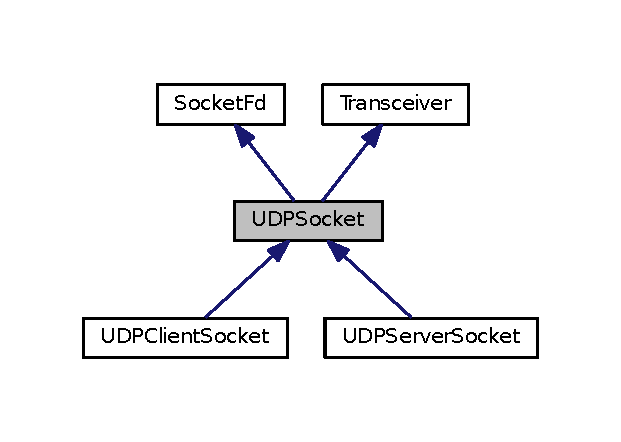
\includegraphics[width=298pt]{classUDPSocket__inherit__graph}
\end{center}
\end{figure}


Collaboration diagram for U\+D\+P\+Socket\+:
\nopagebreak
\begin{figure}[H]
\begin{center}
\leavevmode
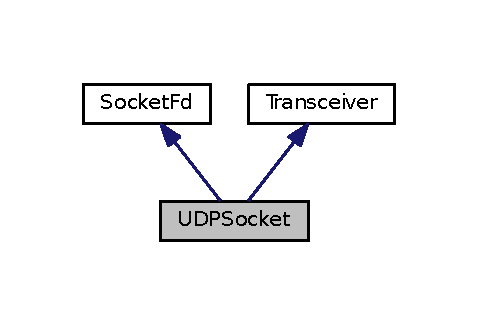
\includegraphics[width=230pt]{classUDPSocket__coll__graph}
\end{center}
\end{figure}
\subsection*{Public Member Functions}
\begin{DoxyCompactItemize}
\item 
int \hyperlink{classUDPSocket_a1c6cf2ad03b21ad00029d5f51fde43f5}{send} (const char $\ast$buf, const unsigned size, int=0)
\begin{DoxyCompactList}\small\item\em Sends Data. \end{DoxyCompactList}\item 
int \hyperlink{classUDPSocket_a712f913657579110edb1f6befbc4a279}{recv} (char $\ast$buf, const unsigned size, int=0)
\begin{DoxyCompactList}\small\item\em Recv Data. \end{DoxyCompactList}\item 
virtual \hyperlink{classUDPSocket_adb1a5254938e5acf5d44ff7a347e9f0a}{$\sim$\+U\+D\+P\+Socket} ()
\begin{DoxyCompactList}\small\item\em frees some structs \end{DoxyCompactList}\end{DoxyCompactItemize}
\subsection*{Protected Member Functions}
\begin{DoxyCompactItemize}
\item 
\hyperlink{classUDPSocket_a4f86f3023f5a08f6355802599a10e100}{U\+D\+P\+Socket} ()
\end{DoxyCompactItemize}
\subsection*{Protected Attributes}
\begin{DoxyCompactItemize}
\item 
int \hyperlink{classUDPSocket_a8b28284b39fbfbd8bca4c1289f7dda32}{rv}
\item 
addrinfo \hyperlink{classUDPSocket_ab0ca283a6135c7073b7a1168014ae088}{hints}
\item 
addrinfo $\ast$ \hyperlink{classUDPSocket_ae0c699a5dbc10580cd2844f282e61f4d}{servinfo}
\item 
addrinfo $\ast$ \hyperlink{classUDPSocket_a9889d73171c2d143797dce81506d24eb}{p}
\item 
sockaddr\+\_\+storage \hyperlink{classUDPSocket_aee1dffc42ebe31dd0400b78d782978de}{their\+\_\+addr}
\end{DoxyCompactItemize}


\subsection{Detailed Description}
virtual baseclass for U\+D\+P Sockets implements \hyperlink{classUDPSocket_a1c6cf2ad03b21ad00029d5f51fde43f5}{send()} and \hyperlink{classUDPSocket_a712f913657579110edb1f6befbc4a279}{recv()} for Client and Server Sockets and holds some structs used by both 

Definition at line 18 of file U\+D\+P\+Socket.\+h.



\subsection{Constructor \& Destructor Documentation}
\hypertarget{classUDPSocket_a4f86f3023f5a08f6355802599a10e100}{\index{U\+D\+P\+Socket@{U\+D\+P\+Socket}!U\+D\+P\+Socket@{U\+D\+P\+Socket}}
\index{U\+D\+P\+Socket@{U\+D\+P\+Socket}!U\+D\+P\+Socket@{U\+D\+P\+Socket}}
\subsubsection[{U\+D\+P\+Socket}]{\setlength{\rightskip}{0pt plus 5cm}U\+D\+P\+Socket\+::\+U\+D\+P\+Socket (
\begin{DoxyParamCaption}
{}
\end{DoxyParamCaption}
)\hspace{0.3cm}{\ttfamily [protected]}}}\label{classUDPSocket_a4f86f3023f5a08f6355802599a10e100}


Definition at line 3 of file U\+D\+P\+Socket.\+cpp.



References p, rv, and servinfo.

\hypertarget{classUDPSocket_adb1a5254938e5acf5d44ff7a347e9f0a}{\index{U\+D\+P\+Socket@{U\+D\+P\+Socket}!````~U\+D\+P\+Socket@{$\sim$\+U\+D\+P\+Socket}}
\index{````~U\+D\+P\+Socket@{$\sim$\+U\+D\+P\+Socket}!U\+D\+P\+Socket@{U\+D\+P\+Socket}}
\subsubsection[{$\sim$\+U\+D\+P\+Socket}]{\setlength{\rightskip}{0pt plus 5cm}U\+D\+P\+Socket\+::$\sim$\+U\+D\+P\+Socket (
\begin{DoxyParamCaption}
{}
\end{DoxyParamCaption}
)\hspace{0.3cm}{\ttfamily [virtual]}}}\label{classUDPSocket_adb1a5254938e5acf5d44ff7a347e9f0a}


frees some structs 

frees some structs 

Definition at line 9 of file U\+D\+P\+Socket.\+cpp.



References servinfo, and Socket\+Fd\+::ufds.



\subsection{Member Function Documentation}
\hypertarget{classUDPSocket_a712f913657579110edb1f6befbc4a279}{\index{U\+D\+P\+Socket@{U\+D\+P\+Socket}!recv@{recv}}
\index{recv@{recv}!U\+D\+P\+Socket@{U\+D\+P\+Socket}}
\subsubsection[{recv}]{\setlength{\rightskip}{0pt plus 5cm}int U\+D\+P\+Socket\+::recv (
\begin{DoxyParamCaption}
\item[{char $\ast$}]{buf, }
\item[{const unsigned}]{size, }
\item[{int}]{ = {\ttfamily 0}}
\end{DoxyParamCaption}
)\hspace{0.3cm}{\ttfamily [virtual]}}}\label{classUDPSocket_a712f913657579110edb1f6befbc4a279}


Recv Data. 

Recv Data 
\begin{DoxyParams}[1]{Parameters}
\mbox{\tt in}  & {\em buf} & recv buffer \\
\hline
\mbox{\tt in}  & {\em size} & nb of bytes to recv \\
\hline
\mbox{\tt in}  & {\em ???} & \\
\hline
\end{DoxyParams}


Implements \hyperlink{classTransceiver_aef7153a423766522f4f82c1300157048}{Transceiver}.



Definition at line 18 of file U\+D\+P\+Socket.\+cpp.



References p, and Socket\+Fd\+::ufds.



Referenced by main().



Here is the caller graph for this function\+:
\nopagebreak
\begin{figure}[H]
\begin{center}
\leavevmode
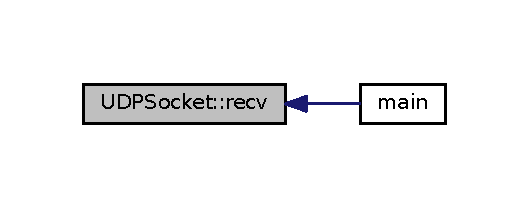
\includegraphics[width=254pt]{classUDPSocket_a712f913657579110edb1f6befbc4a279_icgraph}
\end{center}
\end{figure}


\hypertarget{classUDPSocket_a1c6cf2ad03b21ad00029d5f51fde43f5}{\index{U\+D\+P\+Socket@{U\+D\+P\+Socket}!send@{send}}
\index{send@{send}!U\+D\+P\+Socket@{U\+D\+P\+Socket}}
\subsubsection[{send}]{\setlength{\rightskip}{0pt plus 5cm}int U\+D\+P\+Socket\+::send (
\begin{DoxyParamCaption}
\item[{const char $\ast$}]{buf, }
\item[{const unsigned}]{size, }
\item[{int}]{ = {\ttfamily 0}}
\end{DoxyParamCaption}
)\hspace{0.3cm}{\ttfamily [virtual]}}}\label{classUDPSocket_a1c6cf2ad03b21ad00029d5f51fde43f5}


Sends Data. 

Sends Data 
\begin{DoxyParams}[1]{Parameters}
\mbox{\tt in}  & {\em buf} & send buffer \\
\hline
\mbox{\tt in}  & {\em size} & nb of bytes to send \\
\hline
\mbox{\tt in}  & {\em ???} & \\
\hline
\end{DoxyParams}


Implements \hyperlink{classTransceiver_aa54935e0032d9ab6c531024e001ae19d}{Transceiver}.



Definition at line 14 of file U\+D\+P\+Socket.\+cpp.



References p, and Socket\+Fd\+::ufds.



Referenced by main().



Here is the caller graph for this function\+:
\nopagebreak
\begin{figure}[H]
\begin{center}
\leavevmode
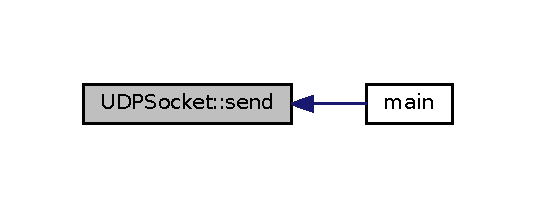
\includegraphics[width=257pt]{classUDPSocket_a1c6cf2ad03b21ad00029d5f51fde43f5_icgraph}
\end{center}
\end{figure}




\subsection{Member Data Documentation}
\hypertarget{classUDPSocket_ab0ca283a6135c7073b7a1168014ae088}{\index{U\+D\+P\+Socket@{U\+D\+P\+Socket}!hints@{hints}}
\index{hints@{hints}!U\+D\+P\+Socket@{U\+D\+P\+Socket}}
\subsubsection[{hints}]{\setlength{\rightskip}{0pt plus 5cm}addrinfo U\+D\+P\+Socket\+::hints\hspace{0.3cm}{\ttfamily [protected]}}}\label{classUDPSocket_ab0ca283a6135c7073b7a1168014ae088}


Definition at line 21 of file U\+D\+P\+Socket.\+h.



Referenced by U\+D\+P\+Client\+Socket\+::\+U\+D\+P\+Client\+Socket(), and U\+D\+P\+Server\+Socket\+::\+U\+D\+P\+Server\+Socket().

\hypertarget{classUDPSocket_a9889d73171c2d143797dce81506d24eb}{\index{U\+D\+P\+Socket@{U\+D\+P\+Socket}!p@{p}}
\index{p@{p}!U\+D\+P\+Socket@{U\+D\+P\+Socket}}
\subsubsection[{p}]{\setlength{\rightskip}{0pt plus 5cm}addrinfo $\ast$ U\+D\+P\+Socket\+::p\hspace{0.3cm}{\ttfamily [protected]}}}\label{classUDPSocket_a9889d73171c2d143797dce81506d24eb}


Definition at line 21 of file U\+D\+P\+Socket.\+h.



Referenced by recv(), send(), U\+D\+P\+Client\+Socket\+::\+U\+D\+P\+Client\+Socket(), U\+D\+P\+Server\+Socket\+::\+U\+D\+P\+Server\+Socket(), and U\+D\+P\+Socket().

\hypertarget{classUDPSocket_a8b28284b39fbfbd8bca4c1289f7dda32}{\index{U\+D\+P\+Socket@{U\+D\+P\+Socket}!rv@{rv}}
\index{rv@{rv}!U\+D\+P\+Socket@{U\+D\+P\+Socket}}
\subsubsection[{rv}]{\setlength{\rightskip}{0pt plus 5cm}int U\+D\+P\+Socket\+::rv\hspace{0.3cm}{\ttfamily [protected]}}}\label{classUDPSocket_a8b28284b39fbfbd8bca4c1289f7dda32}


Definition at line 20 of file U\+D\+P\+Socket.\+h.



Referenced by U\+D\+P\+Client\+Socket\+::\+U\+D\+P\+Client\+Socket(), U\+D\+P\+Server\+Socket\+::\+U\+D\+P\+Server\+Socket(), and U\+D\+P\+Socket().

\hypertarget{classUDPSocket_ae0c699a5dbc10580cd2844f282e61f4d}{\index{U\+D\+P\+Socket@{U\+D\+P\+Socket}!servinfo@{servinfo}}
\index{servinfo@{servinfo}!U\+D\+P\+Socket@{U\+D\+P\+Socket}}
\subsubsection[{servinfo}]{\setlength{\rightskip}{0pt plus 5cm}addrinfo $\ast$ U\+D\+P\+Socket\+::servinfo\hspace{0.3cm}{\ttfamily [protected]}}}\label{classUDPSocket_ae0c699a5dbc10580cd2844f282e61f4d}


Definition at line 21 of file U\+D\+P\+Socket.\+h.



Referenced by U\+D\+P\+Client\+Socket\+::\+U\+D\+P\+Client\+Socket(), U\+D\+P\+Server\+Socket\+::\+U\+D\+P\+Server\+Socket(), U\+D\+P\+Socket(), and $\sim$\+U\+D\+P\+Socket().

\hypertarget{classUDPSocket_aee1dffc42ebe31dd0400b78d782978de}{\index{U\+D\+P\+Socket@{U\+D\+P\+Socket}!their\+\_\+addr@{their\+\_\+addr}}
\index{their\+\_\+addr@{their\+\_\+addr}!U\+D\+P\+Socket@{U\+D\+P\+Socket}}
\subsubsection[{their\+\_\+addr}]{\setlength{\rightskip}{0pt plus 5cm}sockaddr\+\_\+storage U\+D\+P\+Socket\+::their\+\_\+addr\hspace{0.3cm}{\ttfamily [protected]}}}\label{classUDPSocket_aee1dffc42ebe31dd0400b78d782978de}


Definition at line 22 of file U\+D\+P\+Socket.\+h.



The documentation for this class was generated from the following files\+:\begin{DoxyCompactItemize}
\item 
include/\hyperlink{UDPSocket_8h}{U\+D\+P\+Socket.\+h}\item 
src/\hyperlink{UDPSocket_8cpp}{U\+D\+P\+Socket.\+cpp}\end{DoxyCompactItemize}

\hypertarget{classUNIXClientSocket}{\section{U\+N\+I\+X\+Client\+Socket Class Reference}
\label{classUNIXClientSocket}\index{U\+N\+I\+X\+Client\+Socket@{U\+N\+I\+X\+Client\+Socket}}
}


{\ttfamily \#include $<$U\+N\+I\+X\+Client\+Socket.\+h$>$}



Inheritance diagram for U\+N\+I\+X\+Client\+Socket\+:
\nopagebreak
\begin{figure}[H]
\begin{center}
\leavevmode
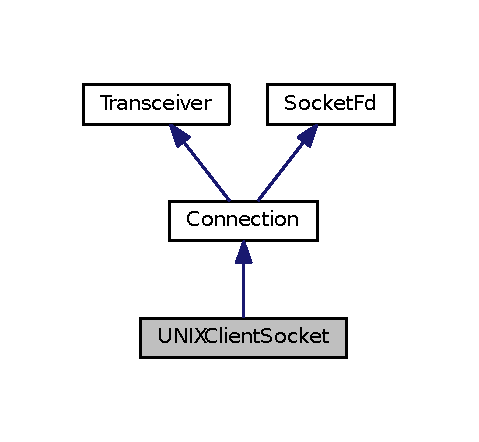
\includegraphics[width=230pt]{classUNIXClientSocket__inherit__graph}
\end{center}
\end{figure}


Collaboration diagram for U\+N\+I\+X\+Client\+Socket\+:
\nopagebreak
\begin{figure}[H]
\begin{center}
\leavevmode
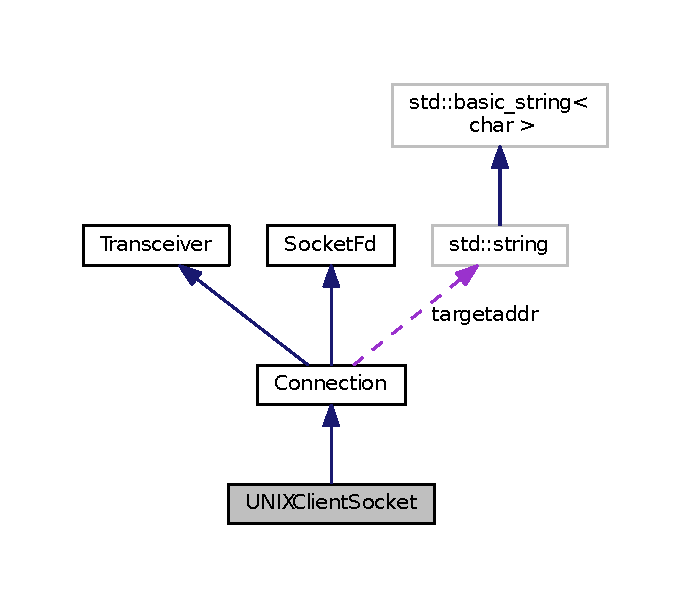
\includegraphics[width=332pt]{classUNIXClientSocket__coll__graph}
\end{center}
\end{figure}
\subsection*{Public Member Functions}
\begin{DoxyCompactItemize}
\item 
\hyperlink{classUNIXClientSocket_a1c1fd48cd60ea3ee5478ae6b238ab376}{U\+N\+I\+X\+Client\+Socket} (const char $\ast$path)
\begin{DoxyCompactList}\small\item\em construct \hyperlink{classUNIXClientSocket}{U\+N\+I\+X\+Client\+Socket} throws runtime\+\_\+error on failure \end{DoxyCompactList}\item 
virtual \hyperlink{classUNIXClientSocket_ade64c842f5dba7948419ebdcbec291d6}{$\sim$\+U\+N\+I\+X\+Client\+Socket} ()
\end{DoxyCompactItemize}
\subsection*{Private Attributes}
\begin{DoxyCompactItemize}
\item 
sockaddr\+\_\+un \hyperlink{classUNIXClientSocket_a78c19c12f8befc559e916b41262d5f6e}{remote}
\end{DoxyCompactItemize}
\subsection*{Additional Inherited Members}


\subsection{Detailed Description}
A \hyperlink{classUNIXClientSocket}{U\+N\+I\+X\+Client\+Socket} establishes a connection on construct Afterwards it can be used like a \hyperlink{classConnection}{Connection} Object. It directly provides \hyperlink{classConnection_a5466a66e569e81d891559686f2c7594b}{send()} and \hyperlink{classConnection_ab16b8a780c69303beec9b1f67fb596f3}{recv()} functions on init/connection error the Constructor throws a std\+::runtime\+\_\+error 

Definition at line 21 of file U\+N\+I\+X\+Client\+Socket.\+h.



\subsection{Constructor \& Destructor Documentation}
\hypertarget{classUNIXClientSocket_a1c1fd48cd60ea3ee5478ae6b238ab376}{\index{U\+N\+I\+X\+Client\+Socket@{U\+N\+I\+X\+Client\+Socket}!U\+N\+I\+X\+Client\+Socket@{U\+N\+I\+X\+Client\+Socket}}
\index{U\+N\+I\+X\+Client\+Socket@{U\+N\+I\+X\+Client\+Socket}!U\+N\+I\+X\+Client\+Socket@{U\+N\+I\+X\+Client\+Socket}}
\subsubsection[{U\+N\+I\+X\+Client\+Socket}]{\setlength{\rightskip}{0pt plus 5cm}U\+N\+I\+X\+Client\+Socket\+::\+U\+N\+I\+X\+Client\+Socket (
\begin{DoxyParamCaption}
\item[{const char $\ast$}]{path}
\end{DoxyParamCaption}
)}}\label{classUNIXClientSocket_a1c1fd48cd60ea3ee5478ae6b238ab376}


construct \hyperlink{classUNIXClientSocket}{U\+N\+I\+X\+Client\+Socket} throws runtime\+\_\+error on failure 

construct \hyperlink{classUNIXClientSocket}{U\+N\+I\+X\+Client\+Socket} throws runtime\+\_\+error on failure 
\begin{DoxyParams}[1]{Parameters}
\mbox{\tt in}  & {\em path} & Path to socket file \\
\hline
\end{DoxyParams}


Definition at line 3 of file U\+N\+I\+X\+Client\+Socket.\+cpp.



References remote, and Socket\+Fd\+::ufds.

\hypertarget{classUNIXClientSocket_ade64c842f5dba7948419ebdcbec291d6}{\index{U\+N\+I\+X\+Client\+Socket@{U\+N\+I\+X\+Client\+Socket}!````~U\+N\+I\+X\+Client\+Socket@{$\sim$\+U\+N\+I\+X\+Client\+Socket}}
\index{````~U\+N\+I\+X\+Client\+Socket@{$\sim$\+U\+N\+I\+X\+Client\+Socket}!U\+N\+I\+X\+Client\+Socket@{U\+N\+I\+X\+Client\+Socket}}
\subsubsection[{$\sim$\+U\+N\+I\+X\+Client\+Socket}]{\setlength{\rightskip}{0pt plus 5cm}U\+N\+I\+X\+Client\+Socket\+::$\sim$\+U\+N\+I\+X\+Client\+Socket (
\begin{DoxyParamCaption}
{}
\end{DoxyParamCaption}
)\hspace{0.3cm}{\ttfamily [virtual]}}}\label{classUNIXClientSocket_ade64c842f5dba7948419ebdcbec291d6}


Definition at line 22 of file U\+N\+I\+X\+Client\+Socket.\+cpp.



\subsection{Member Data Documentation}
\hypertarget{classUNIXClientSocket_a78c19c12f8befc559e916b41262d5f6e}{\index{U\+N\+I\+X\+Client\+Socket@{U\+N\+I\+X\+Client\+Socket}!remote@{remote}}
\index{remote@{remote}!U\+N\+I\+X\+Client\+Socket@{U\+N\+I\+X\+Client\+Socket}}
\subsubsection[{remote}]{\setlength{\rightskip}{0pt plus 5cm}sockaddr\+\_\+un U\+N\+I\+X\+Client\+Socket\+::remote\hspace{0.3cm}{\ttfamily [private]}}}\label{classUNIXClientSocket_a78c19c12f8befc559e916b41262d5f6e}


Definition at line 26 of file U\+N\+I\+X\+Client\+Socket.\+h.



Referenced by U\+N\+I\+X\+Client\+Socket().



The documentation for this class was generated from the following files\+:\begin{DoxyCompactItemize}
\item 
include/\hyperlink{UNIXClientSocket_8h}{U\+N\+I\+X\+Client\+Socket.\+h}\item 
src/\hyperlink{UNIXClientSocket_8cpp}{U\+N\+I\+X\+Client\+Socket.\+cpp}\end{DoxyCompactItemize}

\hypertarget{classUNIXServerSocket}{\section{U\+N\+I\+X\+Server\+Socket Class Reference}
\label{classUNIXServerSocket}\index{U\+N\+I\+X\+Server\+Socket@{U\+N\+I\+X\+Server\+Socket}}
}


{\ttfamily \#include $<$U\+N\+I\+X\+Server\+Socket.\+h$>$}



Inheritance diagram for U\+N\+I\+X\+Server\+Socket\+:
\nopagebreak
\begin{figure}[H]
\begin{center}
\leavevmode
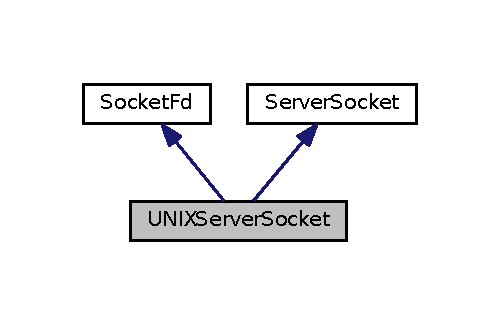
\includegraphics[width=240pt]{classUNIXServerSocket__inherit__graph}
\end{center}
\end{figure}


Collaboration diagram for U\+N\+I\+X\+Server\+Socket\+:
\nopagebreak
\begin{figure}[H]
\begin{center}
\leavevmode
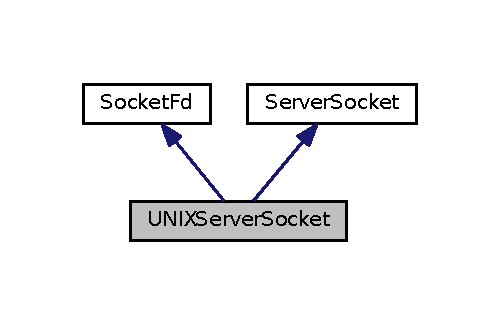
\includegraphics[width=240pt]{classUNIXServerSocket__coll__graph}
\end{center}
\end{figure}
\subsection*{Public Member Functions}
\begin{DoxyCompactItemize}
\item 
\hyperlink{classUNIXServerSocket_a529968cfbf9c158cf5420654b503d4b1}{U\+N\+I\+X\+Server\+Socket} (const char $\ast$path)
\begin{DoxyCompactList}\small\item\em construct a unix server socket \end{DoxyCompactList}\item 
virtual \hyperlink{classUNIXServerSocket_a53d5ee91751f59e2ee719fe074dc468f}{$\sim$\+U\+N\+I\+X\+Server\+Socket} ()
\item 
\hyperlink{classConnection}{Connection} $\ast$ \hyperlink{classUNIXServerSocket_a1bd19b56a910dc3811d4d54c30fbf3f5}{accept} ()
\end{DoxyCompactItemize}
\subsection*{Private Attributes}
\begin{DoxyCompactItemize}
\item 
int \hyperlink{classUNIXServerSocket_ab5864738b5d930ec0cf0017e0a6b4c84}{last\+\_\+new\+\_\+sock}
\item 
sockaddr\+\_\+un \hyperlink{classUNIXServerSocket_a8e6873260b9bb0e49ed09a4d03694044}{local}
\item 
sockaddr\+\_\+un \hyperlink{classUNIXServerSocket_a19d9cd6705ffa42363e04f989b0c4904}{remote}
\end{DoxyCompactItemize}
\subsection*{Additional Inherited Members}


\subsection{Detailed Description}
A \hyperlink{classUNIXServerSocket}{U\+N\+I\+X\+Server\+Socket} provides a means for U\+N\+I\+X Clients to be Accepted with the \hyperlink{classUNIXServerSocket_a1bd19b56a910dc3811d4d54c30fbf3f5}{accept()} methode it provides if the construction failes and the socketfile can not be accessed the constructor will throw a runtime\+\_\+error 

Definition at line 28 of file U\+N\+I\+X\+Server\+Socket.\+h.



\subsection{Constructor \& Destructor Documentation}
\hypertarget{classUNIXServerSocket_a529968cfbf9c158cf5420654b503d4b1}{\index{U\+N\+I\+X\+Server\+Socket@{U\+N\+I\+X\+Server\+Socket}!U\+N\+I\+X\+Server\+Socket@{U\+N\+I\+X\+Server\+Socket}}
\index{U\+N\+I\+X\+Server\+Socket@{U\+N\+I\+X\+Server\+Socket}!U\+N\+I\+X\+Server\+Socket@{U\+N\+I\+X\+Server\+Socket}}
\subsubsection[{U\+N\+I\+X\+Server\+Socket}]{\setlength{\rightskip}{0pt plus 5cm}U\+N\+I\+X\+Server\+Socket\+::\+U\+N\+I\+X\+Server\+Socket (
\begin{DoxyParamCaption}
\item[{const char $\ast$}]{path}
\end{DoxyParamCaption}
)}}\label{classUNIXServerSocket_a529968cfbf9c158cf5420654b503d4b1}


construct a unix server socket 

construct a unix server socket 
\begin{DoxyParams}[1]{Parameters}
\mbox{\tt in}  & {\em path} & Path to U\+N\+I\+X Socket File \\
\hline
\end{DoxyParams}


Definition at line 3 of file U\+N\+I\+X\+Server\+Socket.\+cpp.



References last\+\_\+new\+\_\+sock, local, and Socket\+Fd\+::ufds.

\hypertarget{classUNIXServerSocket_a53d5ee91751f59e2ee719fe074dc468f}{\index{U\+N\+I\+X\+Server\+Socket@{U\+N\+I\+X\+Server\+Socket}!````~U\+N\+I\+X\+Server\+Socket@{$\sim$\+U\+N\+I\+X\+Server\+Socket}}
\index{````~U\+N\+I\+X\+Server\+Socket@{$\sim$\+U\+N\+I\+X\+Server\+Socket}!U\+N\+I\+X\+Server\+Socket@{U\+N\+I\+X\+Server\+Socket}}
\subsubsection[{$\sim$\+U\+N\+I\+X\+Server\+Socket}]{\setlength{\rightskip}{0pt plus 5cm}U\+N\+I\+X\+Server\+Socket\+::$\sim$\+U\+N\+I\+X\+Server\+Socket (
\begin{DoxyParamCaption}
{}
\end{DoxyParamCaption}
)\hspace{0.3cm}{\ttfamily [virtual]}}}\label{classUNIXServerSocket_a53d5ee91751f59e2ee719fe074dc468f}


Definition at line 32 of file U\+N\+I\+X\+Server\+Socket.\+cpp.



References local.



\subsection{Member Function Documentation}
\hypertarget{classUNIXServerSocket_a1bd19b56a910dc3811d4d54c30fbf3f5}{\index{U\+N\+I\+X\+Server\+Socket@{U\+N\+I\+X\+Server\+Socket}!accept@{accept}}
\index{accept@{accept}!U\+N\+I\+X\+Server\+Socket@{U\+N\+I\+X\+Server\+Socket}}
\subsubsection[{accept}]{\setlength{\rightskip}{0pt plus 5cm}{\bf Connection} $\ast$ U\+N\+I\+X\+Server\+Socket\+::accept (
\begin{DoxyParamCaption}
{}
\end{DoxyParamCaption}
)\hspace{0.3cm}{\ttfamily [virtual]}}}\label{classUNIXServerSocket_a1bd19b56a910dc3811d4d54c30fbf3f5}


Implements \hyperlink{classServerSocket_a1d7054bc388f2d789d2124dd96939d90}{Server\+Socket}.



Definition at line 36 of file U\+N\+I\+X\+Server\+Socket.\+cpp.



References last\+\_\+new\+\_\+sock, remote, and Socket\+Fd\+::ufds.



\subsection{Member Data Documentation}
\hypertarget{classUNIXServerSocket_ab5864738b5d930ec0cf0017e0a6b4c84}{\index{U\+N\+I\+X\+Server\+Socket@{U\+N\+I\+X\+Server\+Socket}!last\+\_\+new\+\_\+sock@{last\+\_\+new\+\_\+sock}}
\index{last\+\_\+new\+\_\+sock@{last\+\_\+new\+\_\+sock}!U\+N\+I\+X\+Server\+Socket@{U\+N\+I\+X\+Server\+Socket}}
\subsubsection[{last\+\_\+new\+\_\+sock}]{\setlength{\rightskip}{0pt plus 5cm}int U\+N\+I\+X\+Server\+Socket\+::last\+\_\+new\+\_\+sock\hspace{0.3cm}{\ttfamily [private]}}}\label{classUNIXServerSocket_ab5864738b5d930ec0cf0017e0a6b4c84}


Definition at line 31 of file U\+N\+I\+X\+Server\+Socket.\+h.



Referenced by accept(), and U\+N\+I\+X\+Server\+Socket().

\hypertarget{classUNIXServerSocket_a8e6873260b9bb0e49ed09a4d03694044}{\index{U\+N\+I\+X\+Server\+Socket@{U\+N\+I\+X\+Server\+Socket}!local@{local}}
\index{local@{local}!U\+N\+I\+X\+Server\+Socket@{U\+N\+I\+X\+Server\+Socket}}
\subsubsection[{local}]{\setlength{\rightskip}{0pt plus 5cm}sockaddr\+\_\+un U\+N\+I\+X\+Server\+Socket\+::local\hspace{0.3cm}{\ttfamily [private]}}}\label{classUNIXServerSocket_a8e6873260b9bb0e49ed09a4d03694044}
sockfile structs 

Definition at line 35 of file U\+N\+I\+X\+Server\+Socket.\+h.



Referenced by U\+N\+I\+X\+Server\+Socket(), and $\sim$\+U\+N\+I\+X\+Server\+Socket().

\hypertarget{classUNIXServerSocket_a19d9cd6705ffa42363e04f989b0c4904}{\index{U\+N\+I\+X\+Server\+Socket@{U\+N\+I\+X\+Server\+Socket}!remote@{remote}}
\index{remote@{remote}!U\+N\+I\+X\+Server\+Socket@{U\+N\+I\+X\+Server\+Socket}}
\subsubsection[{remote}]{\setlength{\rightskip}{0pt plus 5cm}sockaddr\+\_\+un U\+N\+I\+X\+Server\+Socket\+::remote\hspace{0.3cm}{\ttfamily [private]}}}\label{classUNIXServerSocket_a19d9cd6705ffa42363e04f989b0c4904}


Definition at line 35 of file U\+N\+I\+X\+Server\+Socket.\+h.



Referenced by accept().



The documentation for this class was generated from the following files\+:\begin{DoxyCompactItemize}
\item 
include/\hyperlink{UNIXServerSocket_8h}{U\+N\+I\+X\+Server\+Socket.\+h}\item 
src/\hyperlink{UNIXServerSocket_8cpp}{U\+N\+I\+X\+Server\+Socket.\+cpp}\end{DoxyCompactItemize}

\chapter{File Documentation}
\hypertarget{Connection_8h}{\section{include/\+Connection.h File Reference}
\label{Connection_8h}\index{include/\+Connection.\+h@{include/\+Connection.\+h}}
}
{\ttfamily \#include $<$stdio.\+h$>$}\\*
{\ttfamily \#include $<$sys/unistd.\+h$>$}\\*
{\ttfamily \#include $<$poll.\+h$>$}\\*
{\ttfamily \#include $<$string$>$}\\*
{\ttfamily \#include $<$Transceiver.\+h$>$}\\*
{\ttfamily \#include $<$Socket\+Fd.\+h$>$}\\*
Include dependency graph for Connection.\+h\+:
\nopagebreak
\begin{figure}[H]
\begin{center}
\leavevmode
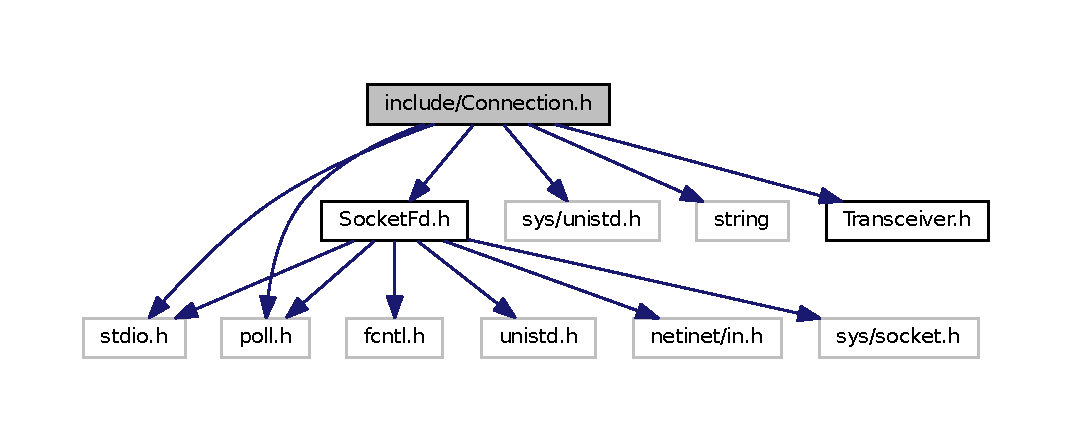
\includegraphics[width=350pt]{Connection_8h__incl}
\end{center}
\end{figure}
This graph shows which files directly or indirectly include this file\+:
\nopagebreak
\begin{figure}[H]
\begin{center}
\leavevmode
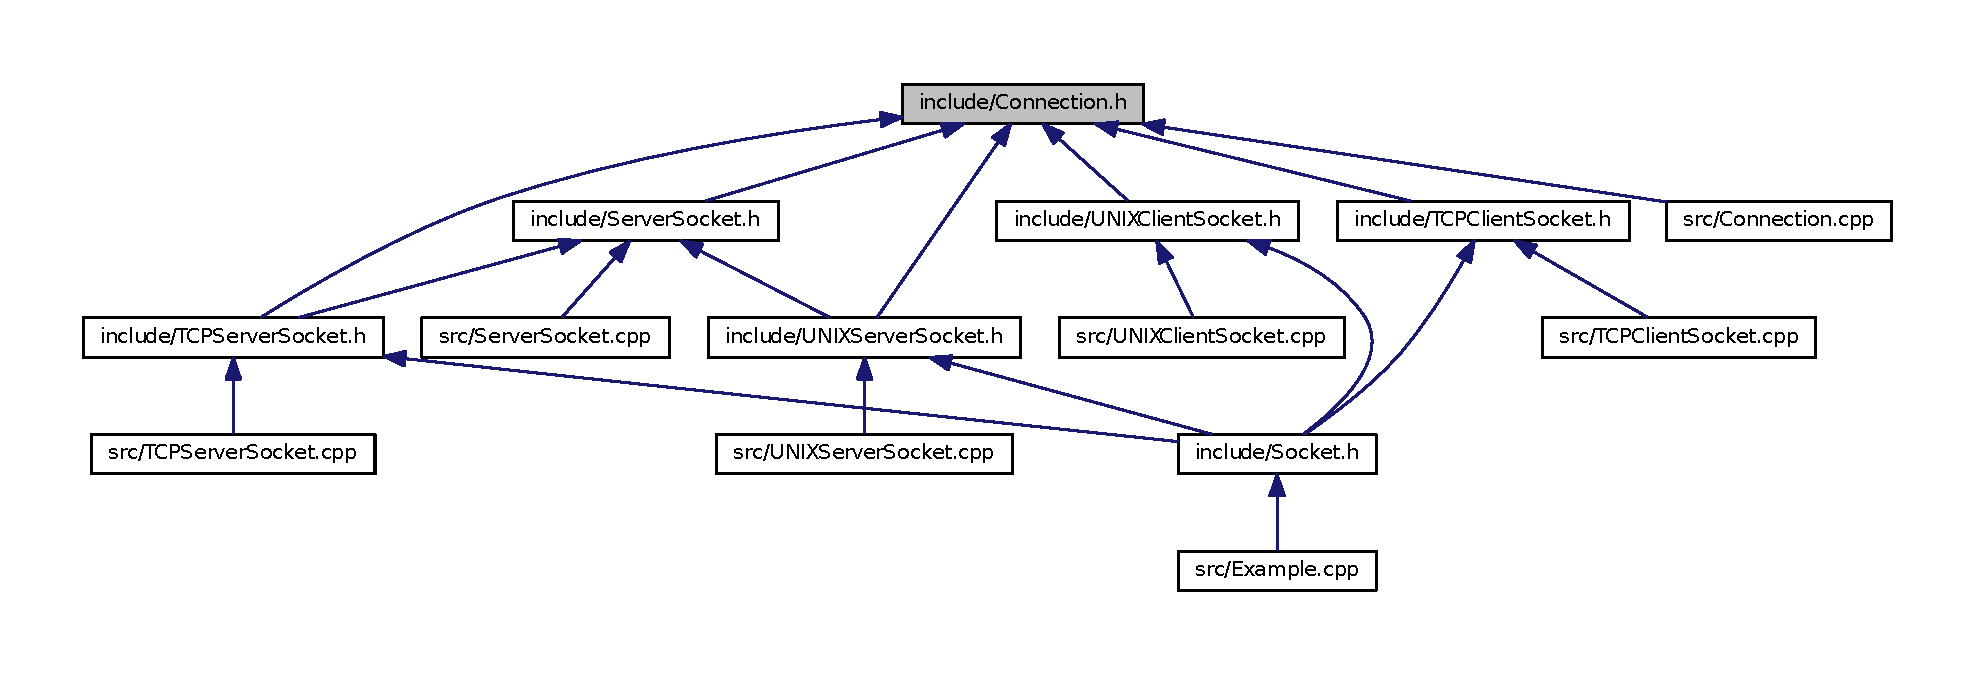
\includegraphics[width=350pt]{Connection_8h__dep__incl}
\end{center}
\end{figure}
\subsection*{Classes}
\begin{DoxyCompactItemize}
\item 
class \hyperlink{classConnection}{Connection}
\end{DoxyCompactItemize}

\hypertarget{ServerSocket_8h}{\section{include/\+Server\+Socket.h File Reference}
\label{ServerSocket_8h}\index{include/\+Server\+Socket.\+h@{include/\+Server\+Socket.\+h}}
}
{\ttfamily \#include $<$Connection.\+h$>$}\\*
Include dependency graph for Server\+Socket.\+h\+:
\nopagebreak
\begin{figure}[H]
\begin{center}
\leavevmode
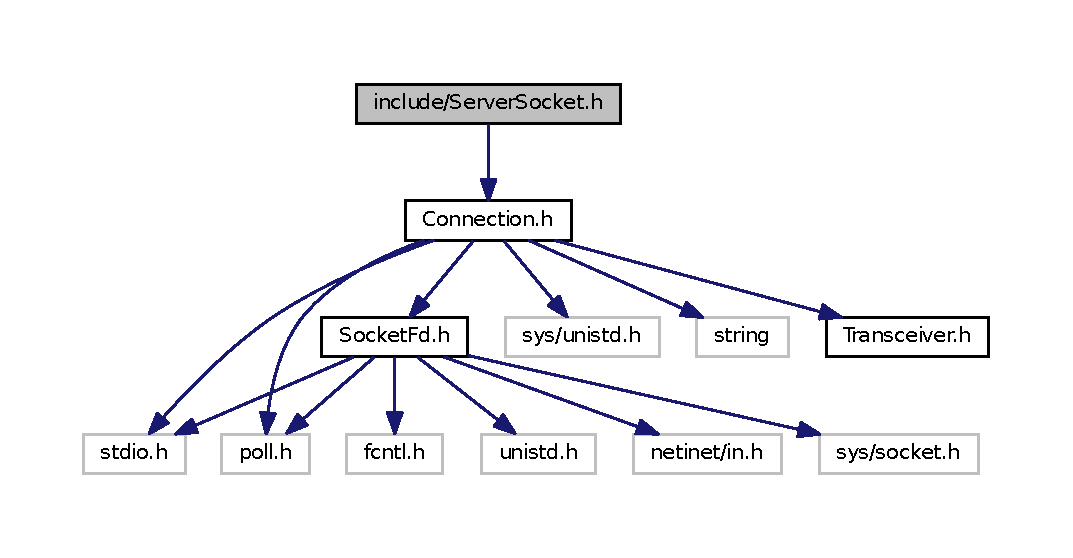
\includegraphics[width=350pt]{ServerSocket_8h__incl}
\end{center}
\end{figure}
This graph shows which files directly or indirectly include this file\+:
\nopagebreak
\begin{figure}[H]
\begin{center}
\leavevmode
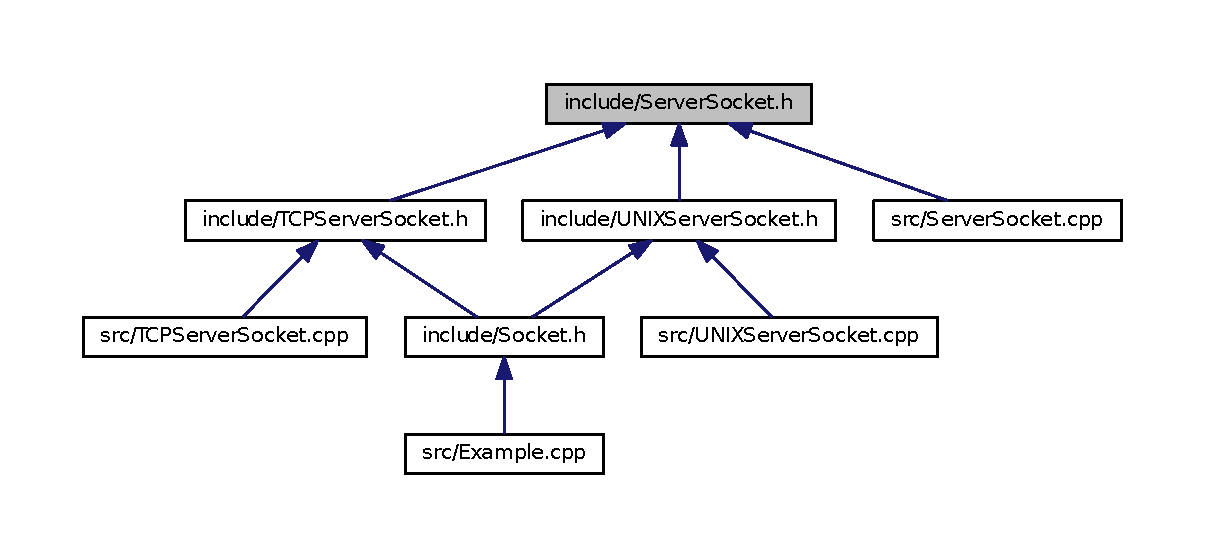
\includegraphics[width=350pt]{ServerSocket_8h__dep__incl}
\end{center}
\end{figure}
\subsection*{Classes}
\begin{DoxyCompactItemize}
\item 
class \hyperlink{classServerSocket}{Server\+Socket}
\begin{DoxyCompactList}\small\item\em Not instanziable Base\+Class for all \hyperlink{classServerSocket}{Server\+Socket} Classes. \end{DoxyCompactList}\end{DoxyCompactItemize}

\hypertarget{Socket_8h}{\section{include/\+Socket.h File Reference}
\label{Socket_8h}\index{include/\+Socket.\+h@{include/\+Socket.\+h}}
}
{\ttfamily \#include $<$T\+C\+P\+Server\+Socket.\+h$>$}\\*
{\ttfamily \#include $<$T\+C\+P\+Client\+Socket.\+h$>$}\\*
{\ttfamily \#include $<$U\+N\+I\+X\+Server\+Socket.\+h$>$}\\*
{\ttfamily \#include $<$U\+N\+I\+X\+Client\+Socket.\+h$>$}\\*
{\ttfamily \#include $<$U\+D\+P\+Server\+Socket.\+h$>$}\\*
{\ttfamily \#include $<$U\+D\+P\+Client\+Socket.\+h$>$}\\*
Include dependency graph for Socket.\+h\+:
\nopagebreak
\begin{figure}[H]
\begin{center}
\leavevmode
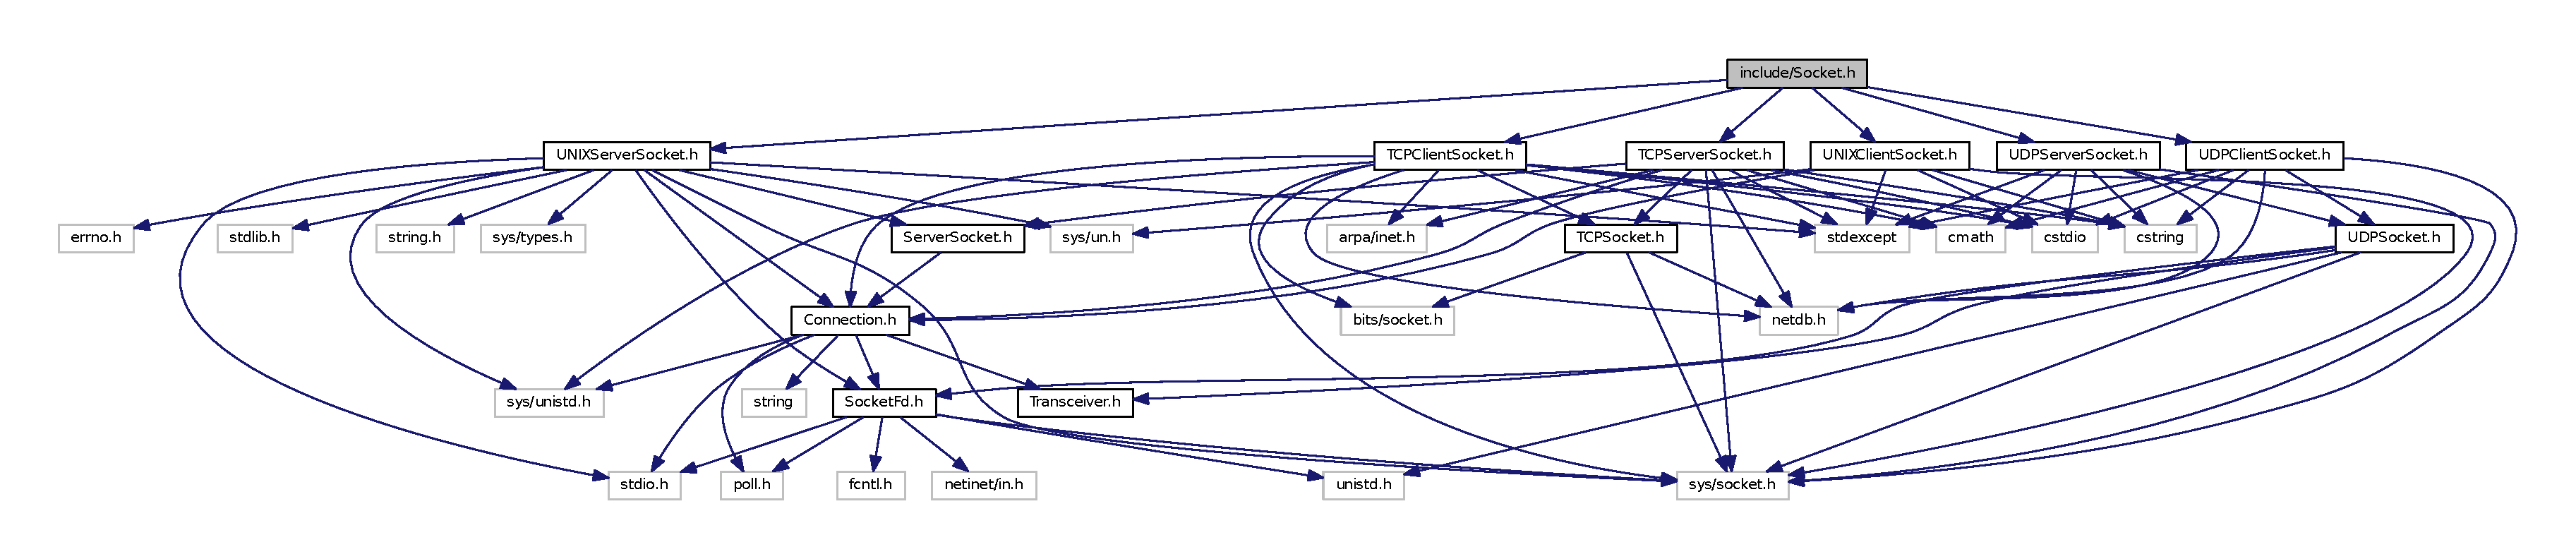
\includegraphics[width=350pt]{Socket_8h__incl}
\end{center}
\end{figure}
This graph shows which files directly or indirectly include this file\+:
\nopagebreak
\begin{figure}[H]
\begin{center}
\leavevmode
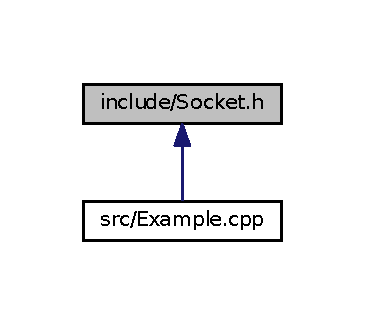
\includegraphics[width=175pt]{Socket_8h__dep__incl}
\end{center}
\end{figure}

\hypertarget{SocketFd_8h}{\section{include/\+Socket\+Fd.h File Reference}
\label{SocketFd_8h}\index{include/\+Socket\+Fd.\+h@{include/\+Socket\+Fd.\+h}}
}
{\ttfamily \#include $<$netinet/in.\+h$>$}\\*
{\ttfamily \#include $<$sys/socket.\+h$>$}\\*
{\ttfamily \#include $<$fcntl.\+h$>$}\\*
{\ttfamily \#include $<$stdio.\+h$>$}\\*
{\ttfamily \#include $<$unistd.\+h$>$}\\*
{\ttfamily \#include $<$poll.\+h$>$}\\*
Include dependency graph for Socket\+Fd.\+h\+:
\nopagebreak
\begin{figure}[H]
\begin{center}
\leavevmode
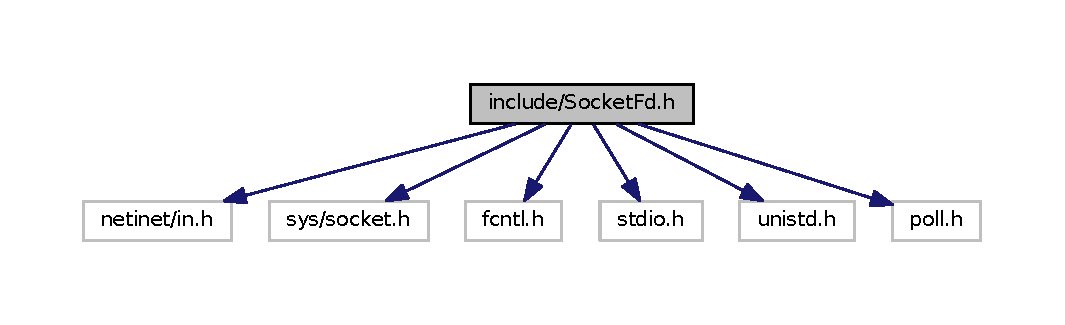
\includegraphics[width=350pt]{SocketFd_8h__incl}
\end{center}
\end{figure}
This graph shows which files directly or indirectly include this file\+:
\nopagebreak
\begin{figure}[H]
\begin{center}
\leavevmode
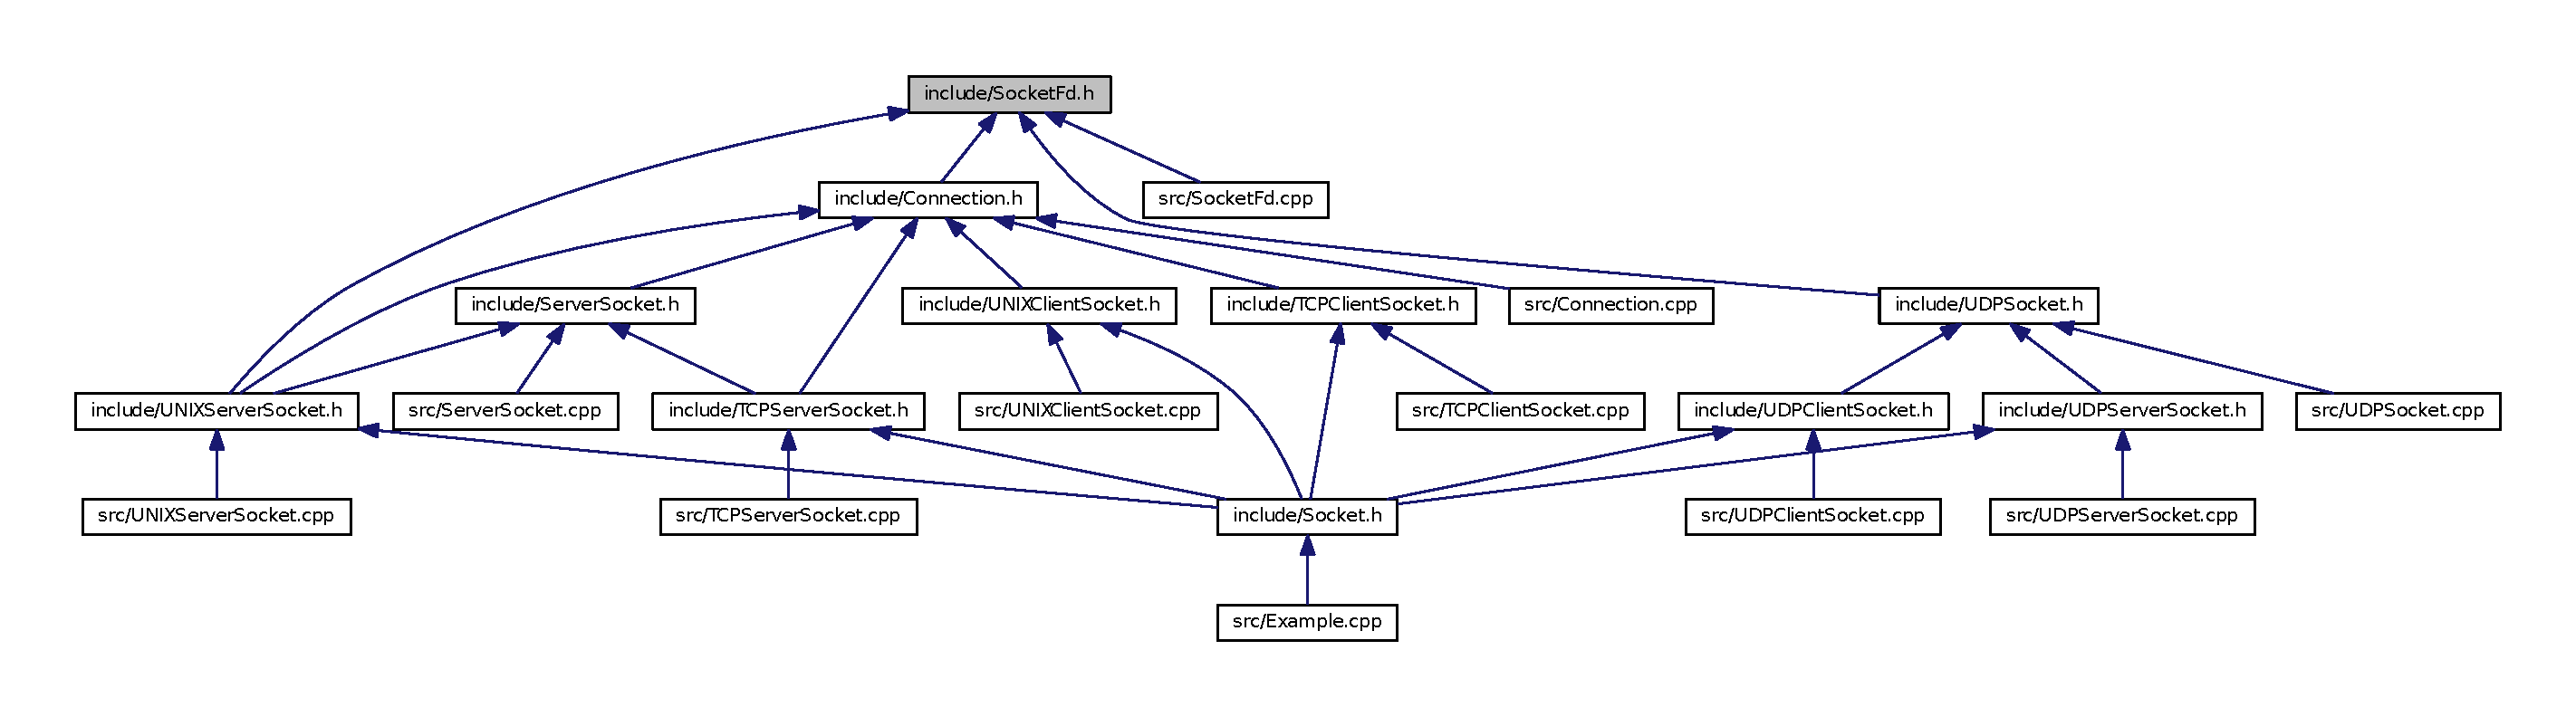
\includegraphics[width=350pt]{SocketFd_8h__dep__incl}
\end{center}
\end{figure}
\subsection*{Classes}
\begin{DoxyCompactItemize}
\item 
class \hyperlink{classSocketFd}{Socket\+Fd}
\begin{DoxyCompactList}\small\item\em Not initalizable Base\+Class for Socket\+File\+Descriptor. \end{DoxyCompactList}\end{DoxyCompactItemize}

\hypertarget{TCPClientSocket_8h}{\section{include/\+T\+C\+P\+Client\+Socket.h File Reference}
\label{TCPClientSocket_8h}\index{include/\+T\+C\+P\+Client\+Socket.\+h@{include/\+T\+C\+P\+Client\+Socket.\+h}}
}
{\ttfamily \#include $<$sys/socket.\+h$>$}\\*
{\ttfamily \#include $<$netdb.\+h$>$}\\*
{\ttfamily \#include $<$bits/socket.\+h$>$}\\*
{\ttfamily \#include $<$sys/unistd.\+h$>$}\\*
{\ttfamily \#include $<$arpa/inet.\+h$>$}\\*
{\ttfamily \#include $<$cstring$>$}\\*
{\ttfamily \#include $<$cmath$>$}\\*
{\ttfamily \#include $<$cstdio$>$}\\*
{\ttfamily \#include $<$stdexcept$>$}\\*
{\ttfamily \#include $<$Connection.\+h$>$}\\*
{\ttfamily \#include $<$T\+C\+P\+Socket.\+h$>$}\\*
Include dependency graph for T\+C\+P\+Client\+Socket.\+h\+:
\nopagebreak
\begin{figure}[H]
\begin{center}
\leavevmode
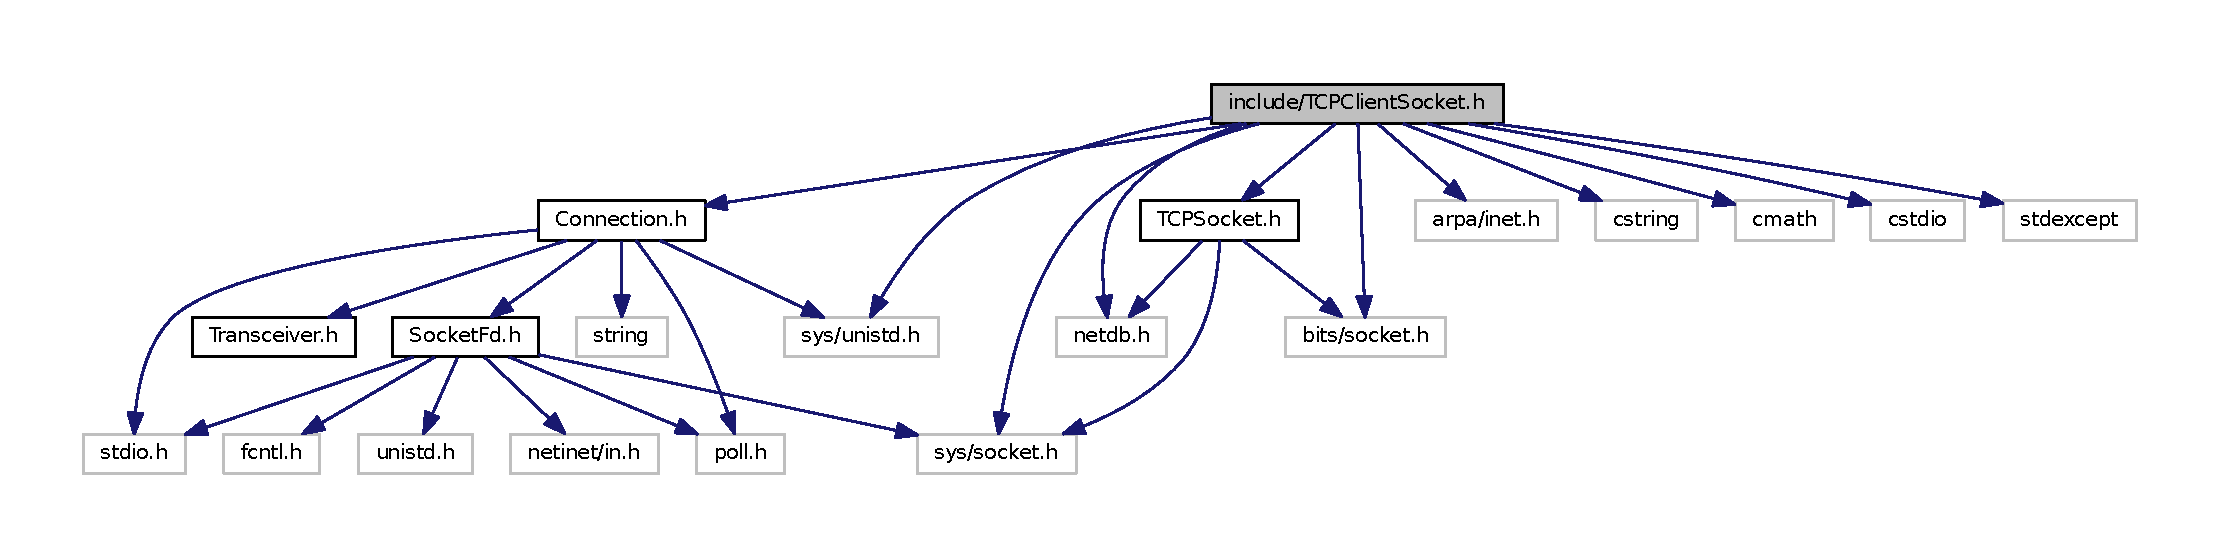
\includegraphics[width=350pt]{TCPClientSocket_8h__incl}
\end{center}
\end{figure}
This graph shows which files directly or indirectly include this file\+:
\nopagebreak
\begin{figure}[H]
\begin{center}
\leavevmode
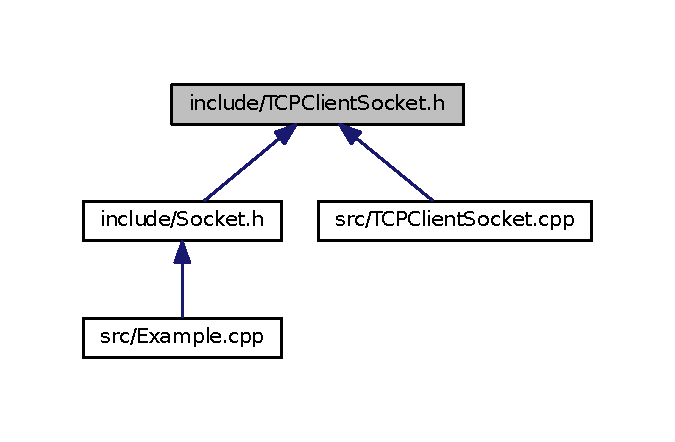
\includegraphics[width=324pt]{TCPClientSocket_8h__dep__incl}
\end{center}
\end{figure}
\subsection*{Classes}
\begin{DoxyCompactItemize}
\item 
class \hyperlink{classTCPClientSocket}{T\+C\+P\+Client\+Socket}
\end{DoxyCompactItemize}

\hypertarget{TCPServerSocket_8h}{\section{include/\+T\+C\+P\+Server\+Socket.h File Reference}
\label{TCPServerSocket_8h}\index{include/\+T\+C\+P\+Server\+Socket.\+h@{include/\+T\+C\+P\+Server\+Socket.\+h}}
}
{\ttfamily \#include $<$sys/socket.\+h$>$}\\*
{\ttfamily \#include $<$netdb.\+h$>$}\\*
{\ttfamily \#include $<$arpa/inet.\+h$>$}\\*
{\ttfamily \#include $<$cstdio$>$}\\*
{\ttfamily \#include $<$cstring$>$}\\*
{\ttfamily \#include $<$cmath$>$}\\*
{\ttfamily \#include $<$stdexcept$>$}\\*
{\ttfamily \#include $<$Connection.\+h$>$}\\*
{\ttfamily \#include $<$T\+C\+P\+Socket.\+h$>$}\\*
{\ttfamily \#include $<$Server\+Socket.\+h$>$}\\*
Include dependency graph for T\+C\+P\+Server\+Socket.\+h\+:
\nopagebreak
\begin{figure}[H]
\begin{center}
\leavevmode
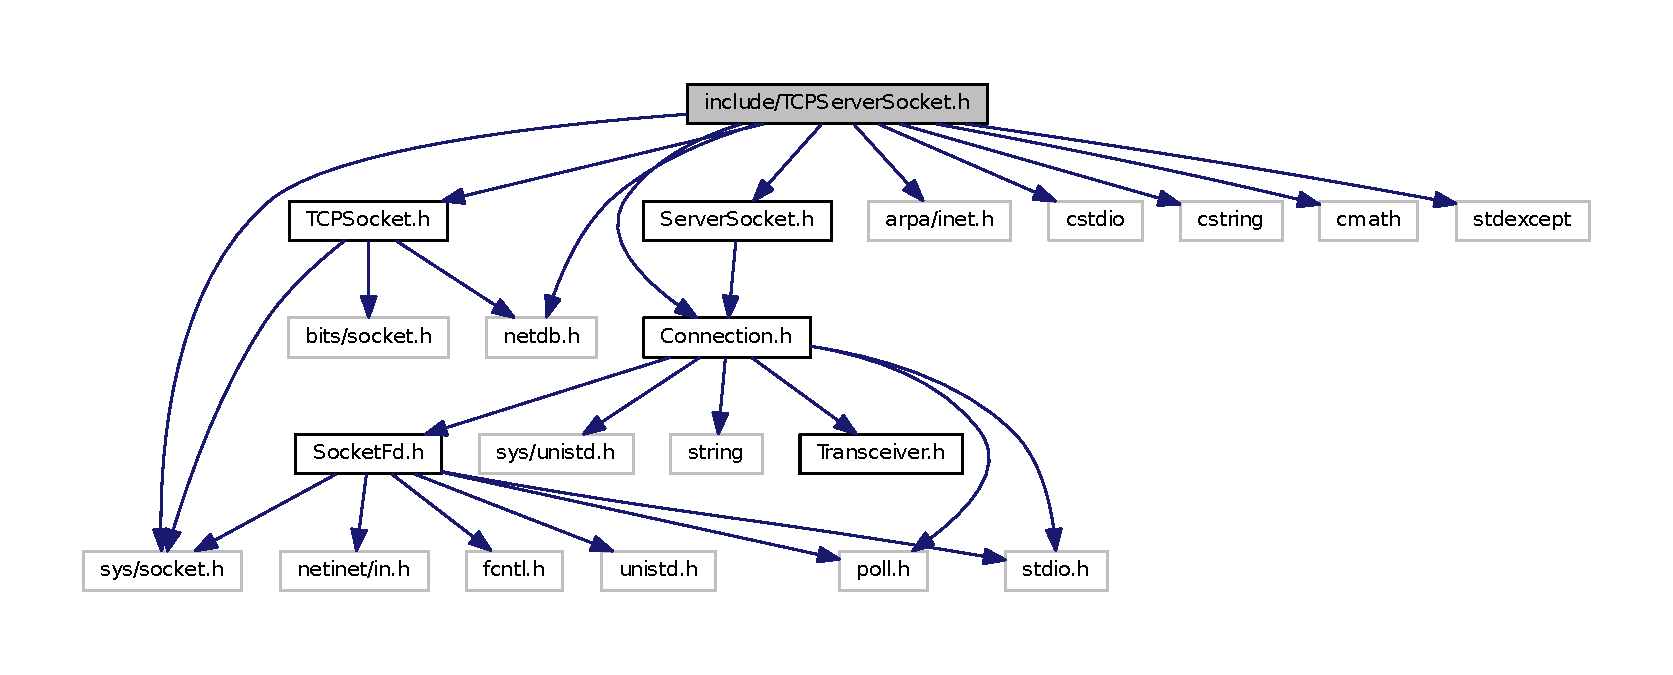
\includegraphics[width=350pt]{TCPServerSocket_8h__incl}
\end{center}
\end{figure}
This graph shows which files directly or indirectly include this file\+:
\nopagebreak
\begin{figure}[H]
\begin{center}
\leavevmode
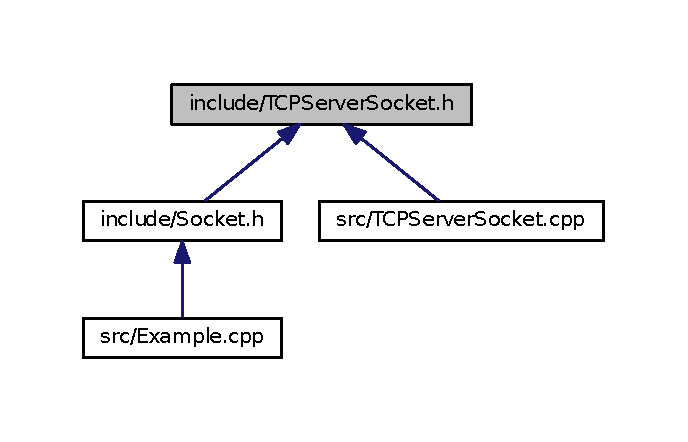
\includegraphics[width=330pt]{TCPServerSocket_8h__dep__incl}
\end{center}
\end{figure}
\subsection*{Classes}
\begin{DoxyCompactItemize}
\item 
class \hyperlink{classTCPServerSocket}{T\+C\+P\+Server\+Socket}
\end{DoxyCompactItemize}

\hypertarget{TCPSocket_8h}{\section{include/\+T\+C\+P\+Socket.h File Reference}
\label{TCPSocket_8h}\index{include/\+T\+C\+P\+Socket.\+h@{include/\+T\+C\+P\+Socket.\+h}}
}
{\ttfamily \#include $<$netdb.\+h$>$}\\*
{\ttfamily \#include $<$bits/socket.\+h$>$}\\*
{\ttfamily \#include $<$sys/socket.\+h$>$}\\*
Include dependency graph for T\+C\+P\+Socket.\+h\+:
\nopagebreak
\begin{figure}[H]
\begin{center}
\leavevmode
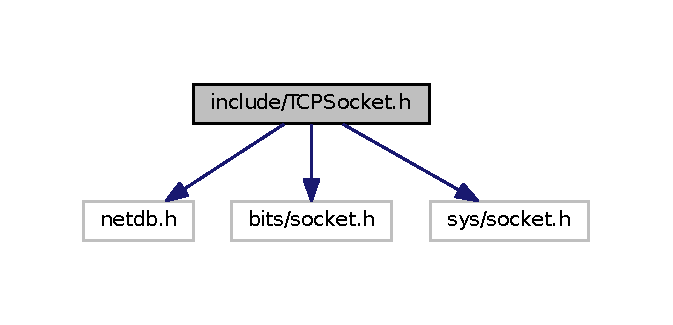
\includegraphics[width=323pt]{TCPSocket_8h__incl}
\end{center}
\end{figure}
This graph shows which files directly or indirectly include this file\+:
\nopagebreak
\begin{figure}[H]
\begin{center}
\leavevmode
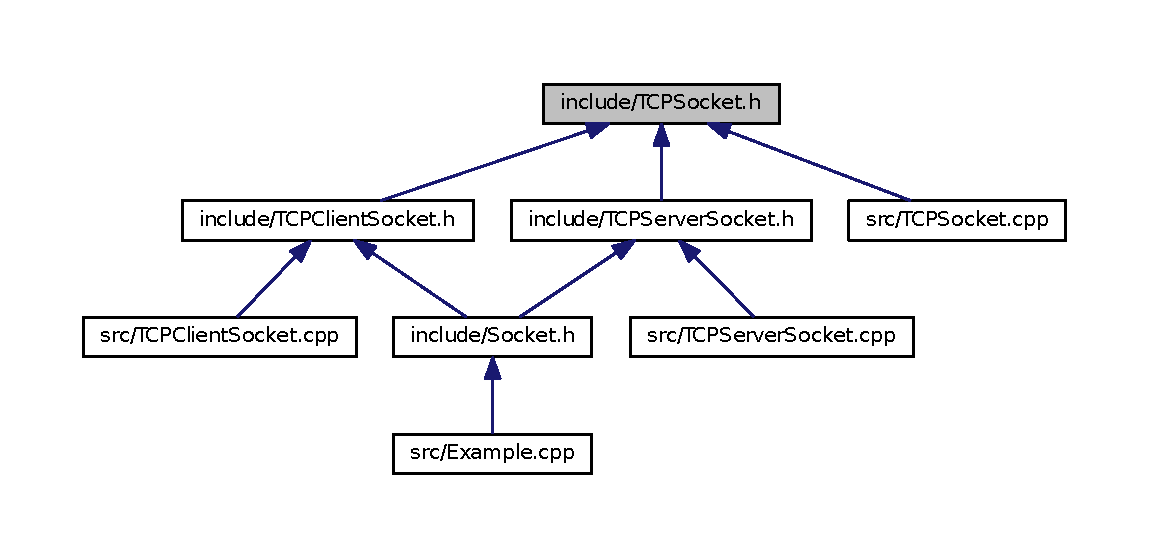
\includegraphics[width=350pt]{TCPSocket_8h__dep__incl}
\end{center}
\end{figure}
\subsection*{Classes}
\begin{DoxyCompactItemize}
\item 
class \hyperlink{classTCPSocket}{T\+C\+P\+Socket}
\end{DoxyCompactItemize}

\hypertarget{Transceiver_8h}{\section{include/\+Transceiver.h File Reference}
\label{Transceiver_8h}\index{include/\+Transceiver.\+h@{include/\+Transceiver.\+h}}
}
This graph shows which files directly or indirectly include this file\+:
\nopagebreak
\begin{figure}[H]
\begin{center}
\leavevmode
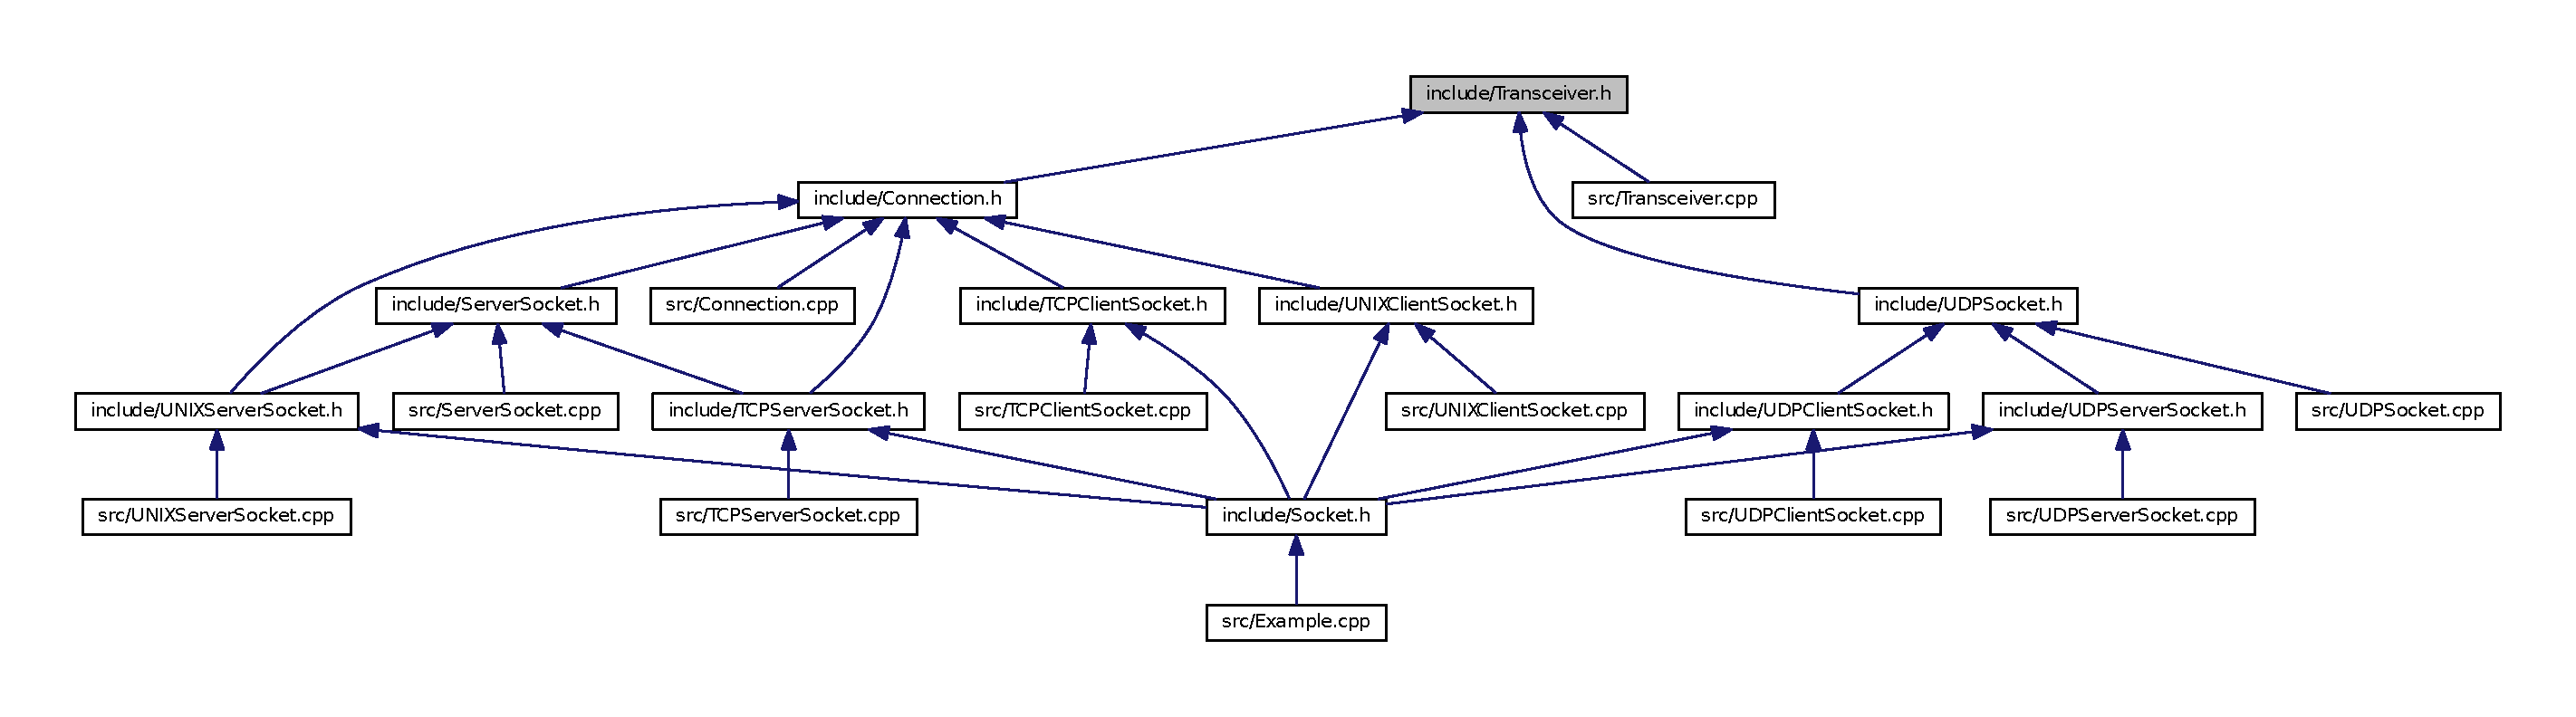
\includegraphics[width=350pt]{Transceiver_8h__dep__incl}
\end{center}
\end{figure}
\subsection*{Classes}
\begin{DoxyCompactItemize}
\item 
class \hyperlink{classTransceiver}{Transceiver}
\end{DoxyCompactItemize}

\hypertarget{UDPClientSocket_8h}{\section{include/\+U\+D\+P\+Client\+Socket.h File Reference}
\label{UDPClientSocket_8h}\index{include/\+U\+D\+P\+Client\+Socket.\+h@{include/\+U\+D\+P\+Client\+Socket.\+h}}
}
{\ttfamily \#include $<$netdb.\+h$>$}\\*
{\ttfamily \#include $<$sys/socket.\+h$>$}\\*
{\ttfamily \#include $<$cmath$>$}\\*
{\ttfamily \#include $<$cstring$>$}\\*
{\ttfamily \#include $<$cstdio$>$}\\*
{\ttfamily \#include $<$stdexcept$>$}\\*
{\ttfamily \#include $<$U\+D\+P\+Socket.\+h$>$}\\*
Include dependency graph for U\+D\+P\+Client\+Socket.\+h\+:
\nopagebreak
\begin{figure}[H]
\begin{center}
\leavevmode
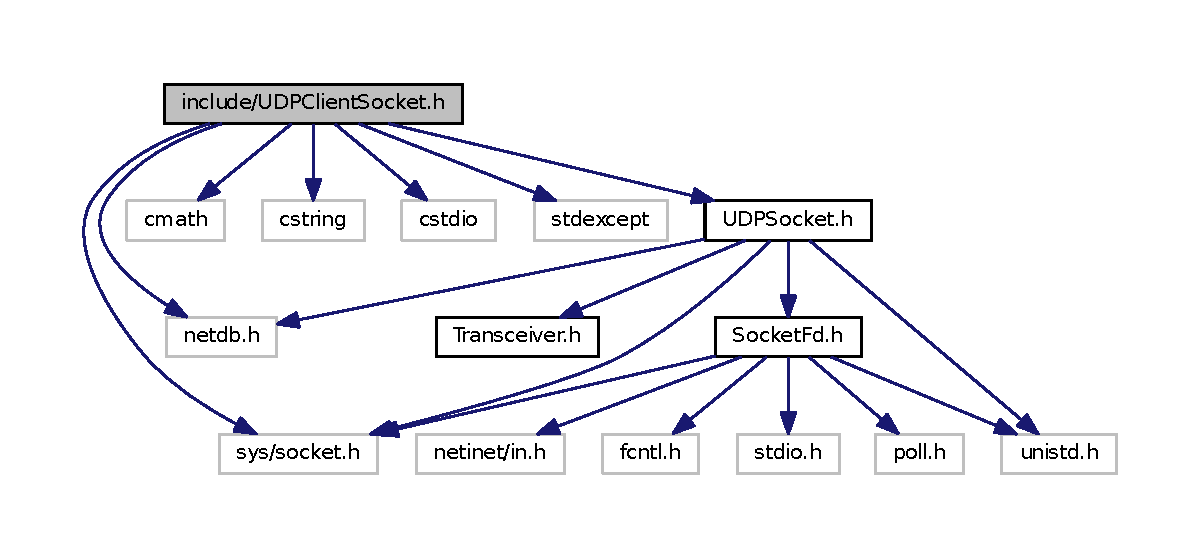
\includegraphics[width=350pt]{UDPClientSocket_8h__incl}
\end{center}
\end{figure}
This graph shows which files directly or indirectly include this file\+:
\nopagebreak
\begin{figure}[H]
\begin{center}
\leavevmode
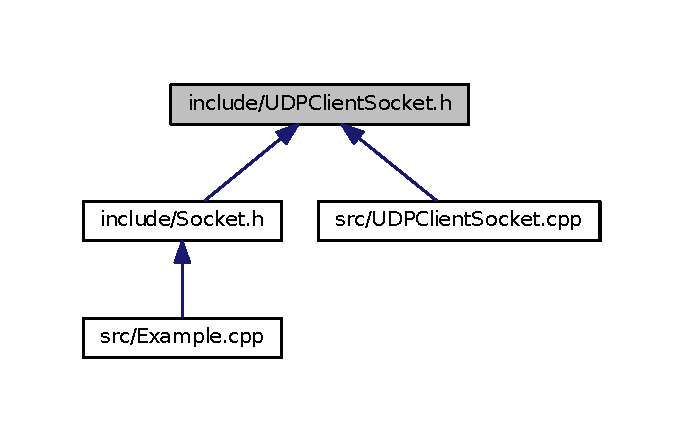
\includegraphics[width=328pt]{UDPClientSocket_8h__dep__incl}
\end{center}
\end{figure}
\subsection*{Classes}
\begin{DoxyCompactItemize}
\item 
class \hyperlink{classUDPClientSocket}{U\+D\+P\+Client\+Socket}
\end{DoxyCompactItemize}

\hypertarget{UDPServerSocket_8h}{\section{include/\+U\+D\+P\+Server\+Socket.h File Reference}
\label{UDPServerSocket_8h}\index{include/\+U\+D\+P\+Server\+Socket.\+h@{include/\+U\+D\+P\+Server\+Socket.\+h}}
}
{\ttfamily \#include $<$netdb.\+h$>$}\\*
{\ttfamily \#include $<$sys/socket.\+h$>$}\\*
{\ttfamily \#include $<$cmath$>$}\\*
{\ttfamily \#include $<$cstring$>$}\\*
{\ttfamily \#include $<$cstdio$>$}\\*
{\ttfamily \#include $<$stdexcept$>$}\\*
{\ttfamily \#include $<$U\+D\+P\+Socket.\+h$>$}\\*
Include dependency graph for U\+D\+P\+Server\+Socket.\+h\+:
\nopagebreak
\begin{figure}[H]
\begin{center}
\leavevmode
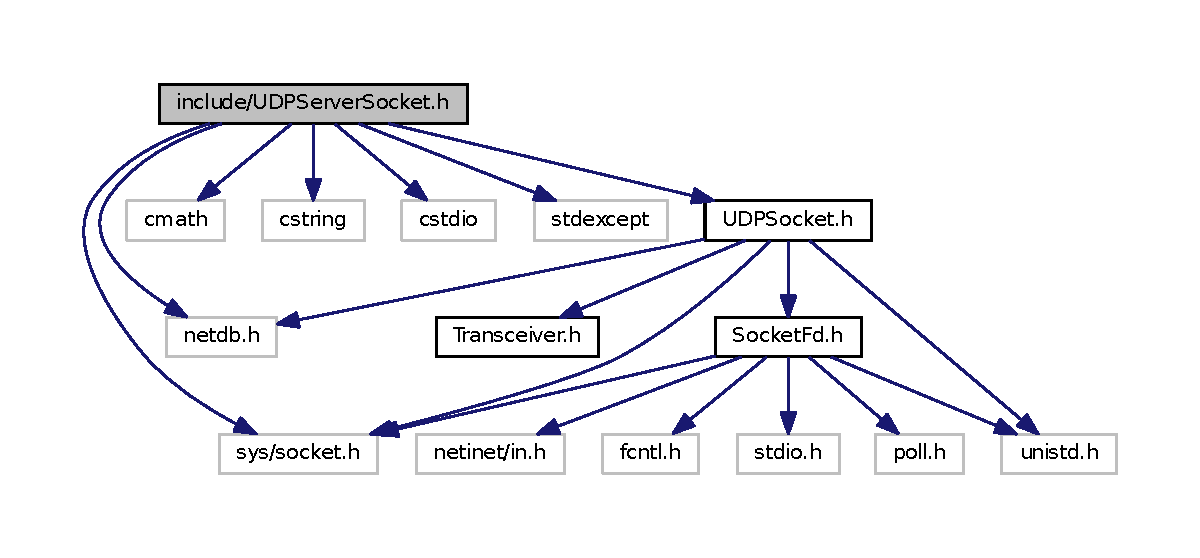
\includegraphics[width=350pt]{UDPServerSocket_8h__incl}
\end{center}
\end{figure}
This graph shows which files directly or indirectly include this file\+:
\nopagebreak
\begin{figure}[H]
\begin{center}
\leavevmode
\includegraphics[width=334pt]{UDPServerSocket_8h__dep__incl}
\end{center}
\end{figure}
\subsection*{Classes}
\begin{DoxyCompactItemize}
\item 
class \hyperlink{classUDPServerSocket}{U\+D\+P\+Server\+Socket}
\end{DoxyCompactItemize}

\hypertarget{UDPSocket_8h}{\section{include/\+U\+D\+P\+Socket.h File Reference}
\label{UDPSocket_8h}\index{include/\+U\+D\+P\+Socket.\+h@{include/\+U\+D\+P\+Socket.\+h}}
}
{\ttfamily \#include $<$unistd.\+h$>$}\\*
{\ttfamily \#include $<$netdb.\+h$>$}\\*
{\ttfamily \#include $<$sys/socket.\+h$>$}\\*
{\ttfamily \#include $<$Transceiver.\+h$>$}\\*
{\ttfamily \#include $<$Socket\+Fd.\+h$>$}\\*
Include dependency graph for U\+D\+P\+Socket.\+h\+:
\nopagebreak
\begin{figure}[H]
\begin{center}
\leavevmode
\includegraphics[width=350pt]{UDPSocket_8h__incl}
\end{center}
\end{figure}
This graph shows which files directly or indirectly include this file\+:
\nopagebreak
\begin{figure}[H]
\begin{center}
\leavevmode
\includegraphics[width=350pt]{UDPSocket_8h__dep__incl}
\end{center}
\end{figure}
\subsection*{Classes}
\begin{DoxyCompactItemize}
\item 
class \hyperlink{classUDPSocket}{U\+D\+P\+Socket}
\end{DoxyCompactItemize}

\hypertarget{UNIXClientSocket_8h}{\section{include/\+U\+N\+I\+X\+Client\+Socket.h File Reference}
\label{UNIXClientSocket_8h}\index{include/\+U\+N\+I\+X\+Client\+Socket.\+h@{include/\+U\+N\+I\+X\+Client\+Socket.\+h}}
}
{\ttfamily \#include $<$sys/socket.\+h$>$}\\*
{\ttfamily \#include $<$sys/un.\+h$>$}\\*
{\ttfamily \#include $<$cstdio$>$}\\*
{\ttfamily \#include $<$cstring$>$}\\*
{\ttfamily \#include $<$stdexcept$>$}\\*
{\ttfamily \#include $<$Connection.\+h$>$}\\*
Include dependency graph for U\+N\+I\+X\+Client\+Socket.\+h\+:
\nopagebreak
\begin{figure}[H]
\begin{center}
\leavevmode
\includegraphics[width=350pt]{UNIXClientSocket_8h__incl}
\end{center}
\end{figure}
This graph shows which files directly or indirectly include this file\+:
\nopagebreak
\begin{figure}[H]
\begin{center}
\leavevmode
\includegraphics[width=330pt]{UNIXClientSocket_8h__dep__incl}
\end{center}
\end{figure}
\subsection*{Classes}
\begin{DoxyCompactItemize}
\item 
class \hyperlink{classUNIXClientSocket}{U\+N\+I\+X\+Client\+Socket}
\end{DoxyCompactItemize}

\hypertarget{UNIXServerSocket_8h}{\section{include/\+U\+N\+I\+X\+Server\+Socket.h File Reference}
\label{UNIXServerSocket_8h}\index{include/\+U\+N\+I\+X\+Server\+Socket.\+h@{include/\+U\+N\+I\+X\+Server\+Socket.\+h}}
}
{\ttfamily \#include $<$sys/unistd.\+h$>$}\\*
{\ttfamily \#include $<$errno.\+h$>$}\\*
{\ttfamily \#include $<$stdio.\+h$>$}\\*
{\ttfamily \#include $<$stdlib.\+h$>$}\\*
{\ttfamily \#include $<$string.\+h$>$}\\*
{\ttfamily \#include $<$sys/types.\+h$>$}\\*
{\ttfamily \#include $<$sys/socket.\+h$>$}\\*
{\ttfamily \#include $<$sys/un.\+h$>$}\\*
{\ttfamily \#include $<$stdexcept$>$}\\*
{\ttfamily \#include $<$Socket\+Fd.\+h$>$}\\*
{\ttfamily \#include $<$Connection.\+h$>$}\\*
{\ttfamily \#include $<$Server\+Socket.\+h$>$}\\*
Include dependency graph for U\+N\+I\+X\+Server\+Socket.\+h\+:
\nopagebreak
\begin{figure}[H]
\begin{center}
\leavevmode
\includegraphics[width=350pt]{UNIXServerSocket_8h__incl}
\end{center}
\end{figure}
This graph shows which files directly or indirectly include this file\+:
\nopagebreak
\begin{figure}[H]
\begin{center}
\leavevmode
\includegraphics[width=336pt]{UNIXServerSocket_8h__dep__incl}
\end{center}
\end{figure}
\subsection*{Classes}
\begin{DoxyCompactItemize}
\item 
class \hyperlink{classUNIXServerSocket}{U\+N\+I\+X\+Server\+Socket}
\end{DoxyCompactItemize}

\hypertarget{Connection_8cpp}{\section{src/\+Connection.cpp File Reference}
\label{Connection_8cpp}\index{src/\+Connection.\+cpp@{src/\+Connection.\+cpp}}
}
{\ttfamily \#include $<$Connection.\+h$>$}\\*
Include dependency graph for Connection.\+cpp\+:
\nopagebreak
\begin{figure}[H]
\begin{center}
\leavevmode
\includegraphics[width=350pt]{Connection_8cpp__incl}
\end{center}
\end{figure}
\subsection*{Macros}
\begin{DoxyCompactItemize}
\item 
\#define \hyperlink{Connection_8cpp_a591f79219998eb65aeacbd25e4459fee}{W\+E\+A\+D\+M\+A\+C\+R\+O}(function)
\end{DoxyCompactItemize}


\subsection{Macro Definition Documentation}
\hypertarget{Connection_8cpp_a591f79219998eb65aeacbd25e4459fee}{\index{Connection.\+cpp@{Connection.\+cpp}!W\+E\+A\+D\+M\+A\+C\+R\+O@{W\+E\+A\+D\+M\+A\+C\+R\+O}}
\index{W\+E\+A\+D\+M\+A\+C\+R\+O@{W\+E\+A\+D\+M\+A\+C\+R\+O}!Connection.\+cpp@{Connection.\+cpp}}
\subsubsection[{W\+E\+A\+D\+M\+A\+C\+R\+O}]{\setlength{\rightskip}{0pt plus 5cm}\#define W\+E\+A\+D\+M\+A\+C\+R\+O(
\begin{DoxyParamCaption}
\item[{}]{function}
\end{DoxyParamCaption}
)}}\label{Connection_8cpp_a591f79219998eb65aeacbd25e4459fee}
{\bfseries Value\+:}
\begin{DoxyCode}
n = sum = 0; \(\backslash\)
do \{ \(\backslash\)
        n = ::function(ufds.fd, buf + sum, size - sum); \(\backslash\)
        if (n == 0) \{ \(\backslash\)
                return (sum); \textcolor{comment}{/* End of File/Stream */}\(\backslash\)
        \} \textcolor{keywordflow}{else} \textcolor{keywordflow}{if} (n < 0) \{ \(\backslash\)
                ::perror(#\textcolor{keyword}{function}); \(\backslash\)
                return (-1); \textcolor{comment}{/* Error */}\(\backslash\)
        \} \textcolor{keywordflow}{else} \{ \(\backslash\)
                sum += n; \(\backslash\)
        \} \(\backslash\)
\} \textcolor{keywordflow}{while} (sum < size); \(\backslash\)
return (sum); \(\backslash\)
\end{DoxyCode}


Definition at line 14 of file Connection.\+cpp.



Referenced by Connection\+::recv(), and Connection\+::send().


\hypertarget{Example_8cpp}{\section{src/\+Example.cpp File Reference}
\label{Example_8cpp}\index{src/\+Example.\+cpp@{src/\+Example.\+cpp}}
}
{\ttfamily \#include $<$iostream$>$}\\*
{\ttfamily \#include $<$Socket.\+h$>$}\\*
{\ttfamily \#include $<$string$>$}\\*
{\ttfamily \#include $<$sstream$>$}\\*
Include dependency graph for Example.\+cpp\+:
\nopagebreak
\begin{figure}[H]
\begin{center}
\leavevmode
\includegraphics[width=350pt]{Example_8cpp__incl}
\end{center}
\end{figure}
\subsection*{Macros}
\begin{DoxyCompactItemize}
\item 
\#define \hyperlink{Example_8cpp_a3db4dba8d56385b62759b89c98cae447}{D\+E\+F\+A\+U\+L\+T\+P\+O\+R\+T}~1234
\item 
\#define \hyperlink{Example_8cpp_a2ebdb9c4431e687bca05e90494a8460b}{D\+E\+F\+A\+U\+L\+T\+M\+S\+G\+C}~\char`\"{}Hello here Client\char`\"{}
\item 
\#define \hyperlink{Example_8cpp_a633fc7423e7d6c4d439c873fec3537ed}{D\+E\+F\+A\+U\+L\+T\+M\+S\+G\+S}~\char`\"{}Hello here Server\char`\"{}
\item 
\#define \hyperlink{Example_8cpp_a36983429d17cdac7405dcd532e65bbc0}{D\+E\+F\+A\+U\+L\+T\+U\+N\+I\+X}~\char`\"{}echo\+\_\+socket\char`\"{}
\item 
\#define \hyperlink{Example_8cpp_aba523120730c0e69e2879d6d60d5377e}{D\+E\+F\+A\+U\+L\+T\+S\+E\+R\+V}~\char`\"{}127.\+0.\+0.\+1\char`\"{}
\end{DoxyCompactItemize}
\subsection*{Functions}
\begin{DoxyCompactItemize}
\item 
void \hyperlink{Example_8cpp_ae0f14589015e103d1db9167bb89e4f4e}{stream\+\_\+server} (\hyperlink{classServerSocket}{Server\+Socket} \&)
\item 
void \hyperlink{Example_8cpp_ac5de2785666f2fc48e9f23fc7da9e895}{stream\+\_\+client} (\hyperlink{classConnection}{Connection} \&)
\item 
string \hyperlink{Example_8cpp_a3894a70718f272b0b2dc91f3b1a3080b}{ltrim} (const string str)
\begin{DoxyCompactList}\small\item\em Removes leading Spaces and Tabs. \end{DoxyCompactList}\item 
string \hyperlink{Example_8cpp_a46d443837f44dcac80a4f1954ca18af8}{rtrim} (const string str)
\begin{DoxyCompactList}\small\item\em Removes trailing Spaces and Tabs. \end{DoxyCompactList}\item 
string \hyperlink{Example_8cpp_a96815f680b2b4c13e5702d35bb956a2e}{trim} (const string str)
\begin{DoxyCompactList}\small\item\em Removes leading and trailing Spaces and Tabs. \end{DoxyCompactList}\item 
{\footnotesize template$<$class T $>$ }\\T \hyperlink{Example_8cpp_a0730396a463e99f15b97d645e826bd76}{str2} (const string str)
\begin{DoxyCompactList}\small\item\em Convert a String to a T Object. \end{DoxyCompactList}\item 
void \hyperlink{Example_8cpp_a52cfa7921b503785d36d8fc027f0f9c3}{printusage} (char $\ast$name)
\begin{DoxyCompactList}\small\item\em prints usage info \end{DoxyCompactList}\item 
int \hyperlink{Example_8cpp_a0ddf1224851353fc92bfbff6f499fa97}{main} (int argc, char $\ast$argv\mbox{[}$\,$\mbox{]})
\end{DoxyCompactItemize}
\subsection*{Variables}
\begin{DoxyCompactItemize}
\item 
static const char \hyperlink{Example_8cpp_ac609d746ffb14c438b9af8060e00a129}{E\+N\+D\+\_\+\+O\+F\+\_\+\+M\+E\+S\+S\+A\+G\+E} = '\textbackslash{}n'
\end{DoxyCompactItemize}


\subsection{Macro Definition Documentation}
\hypertarget{Example_8cpp_a2ebdb9c4431e687bca05e90494a8460b}{\index{Example.\+cpp@{Example.\+cpp}!D\+E\+F\+A\+U\+L\+T\+M\+S\+G\+C@{D\+E\+F\+A\+U\+L\+T\+M\+S\+G\+C}}
\index{D\+E\+F\+A\+U\+L\+T\+M\+S\+G\+C@{D\+E\+F\+A\+U\+L\+T\+M\+S\+G\+C}!Example.\+cpp@{Example.\+cpp}}
\subsubsection[{D\+E\+F\+A\+U\+L\+T\+M\+S\+G\+C}]{\setlength{\rightskip}{0pt plus 5cm}\#define D\+E\+F\+A\+U\+L\+T\+M\+S\+G\+C~\char`\"{}Hello here Client\char`\"{}}}\label{Example_8cpp_a2ebdb9c4431e687bca05e90494a8460b}


Definition at line 21 of file Example.\+cpp.



Referenced by main(), and stream\+\_\+client().

\hypertarget{Example_8cpp_a633fc7423e7d6c4d439c873fec3537ed}{\index{Example.\+cpp@{Example.\+cpp}!D\+E\+F\+A\+U\+L\+T\+M\+S\+G\+S@{D\+E\+F\+A\+U\+L\+T\+M\+S\+G\+S}}
\index{D\+E\+F\+A\+U\+L\+T\+M\+S\+G\+S@{D\+E\+F\+A\+U\+L\+T\+M\+S\+G\+S}!Example.\+cpp@{Example.\+cpp}}
\subsubsection[{D\+E\+F\+A\+U\+L\+T\+M\+S\+G\+S}]{\setlength{\rightskip}{0pt plus 5cm}\#define D\+E\+F\+A\+U\+L\+T\+M\+S\+G\+S~\char`\"{}Hello here Server\char`\"{}}}\label{Example_8cpp_a633fc7423e7d6c4d439c873fec3537ed}


Definition at line 22 of file Example.\+cpp.



Referenced by main(), and stream\+\_\+server().

\hypertarget{Example_8cpp_a3db4dba8d56385b62759b89c98cae447}{\index{Example.\+cpp@{Example.\+cpp}!D\+E\+F\+A\+U\+L\+T\+P\+O\+R\+T@{D\+E\+F\+A\+U\+L\+T\+P\+O\+R\+T}}
\index{D\+E\+F\+A\+U\+L\+T\+P\+O\+R\+T@{D\+E\+F\+A\+U\+L\+T\+P\+O\+R\+T}!Example.\+cpp@{Example.\+cpp}}
\subsubsection[{D\+E\+F\+A\+U\+L\+T\+P\+O\+R\+T}]{\setlength{\rightskip}{0pt plus 5cm}\#define D\+E\+F\+A\+U\+L\+T\+P\+O\+R\+T~1234}}\label{Example_8cpp_a3db4dba8d56385b62759b89c98cae447}


Definition at line 20 of file Example.\+cpp.



Referenced by main().

\hypertarget{Example_8cpp_aba523120730c0e69e2879d6d60d5377e}{\index{Example.\+cpp@{Example.\+cpp}!D\+E\+F\+A\+U\+L\+T\+S\+E\+R\+V@{D\+E\+F\+A\+U\+L\+T\+S\+E\+R\+V}}
\index{D\+E\+F\+A\+U\+L\+T\+S\+E\+R\+V@{D\+E\+F\+A\+U\+L\+T\+S\+E\+R\+V}!Example.\+cpp@{Example.\+cpp}}
\subsubsection[{D\+E\+F\+A\+U\+L\+T\+S\+E\+R\+V}]{\setlength{\rightskip}{0pt plus 5cm}\#define D\+E\+F\+A\+U\+L\+T\+S\+E\+R\+V~\char`\"{}127.\+0.\+0.\+1\char`\"{}}}\label{Example_8cpp_aba523120730c0e69e2879d6d60d5377e}


Definition at line 24 of file Example.\+cpp.



Referenced by main().

\hypertarget{Example_8cpp_a36983429d17cdac7405dcd532e65bbc0}{\index{Example.\+cpp@{Example.\+cpp}!D\+E\+F\+A\+U\+L\+T\+U\+N\+I\+X@{D\+E\+F\+A\+U\+L\+T\+U\+N\+I\+X}}
\index{D\+E\+F\+A\+U\+L\+T\+U\+N\+I\+X@{D\+E\+F\+A\+U\+L\+T\+U\+N\+I\+X}!Example.\+cpp@{Example.\+cpp}}
\subsubsection[{D\+E\+F\+A\+U\+L\+T\+U\+N\+I\+X}]{\setlength{\rightskip}{0pt plus 5cm}\#define D\+E\+F\+A\+U\+L\+T\+U\+N\+I\+X~\char`\"{}echo\+\_\+socket\char`\"{}}}\label{Example_8cpp_a36983429d17cdac7405dcd532e65bbc0}


Definition at line 23 of file Example.\+cpp.



Referenced by main().



\subsection{Function Documentation}
\hypertarget{Example_8cpp_a3894a70718f272b0b2dc91f3b1a3080b}{\index{Example.\+cpp@{Example.\+cpp}!ltrim@{ltrim}}
\index{ltrim@{ltrim}!Example.\+cpp@{Example.\+cpp}}
\subsubsection[{ltrim}]{\setlength{\rightskip}{0pt plus 5cm}string ltrim (
\begin{DoxyParamCaption}
\item[{const string}]{str}
\end{DoxyParamCaption}
)}}\label{Example_8cpp_a3894a70718f272b0b2dc91f3b1a3080b}


Removes leading Spaces and Tabs. 

Removes leading Spaces and Tabs 
\begin{DoxyParams}[1]{Parameters}
\mbox{\tt in}  & {\em str} & String to \\
\hline
\end{DoxyParams}
\begin{DoxyReturn}{Returns}
trimmed String 
\end{DoxyReturn}


Definition at line 382 of file Example.\+cpp.



Referenced by trim().



Here is the caller graph for this function\+:
\nopagebreak
\begin{figure}[H]
\begin{center}
\leavevmode
\includegraphics[width=267pt]{Example_8cpp_a3894a70718f272b0b2dc91f3b1a3080b_icgraph}
\end{center}
\end{figure}


\hypertarget{Example_8cpp_a0ddf1224851353fc92bfbff6f499fa97}{\index{Example.\+cpp@{Example.\+cpp}!main@{main}}
\index{main@{main}!Example.\+cpp@{Example.\+cpp}}
\subsubsection[{main}]{\setlength{\rightskip}{0pt plus 5cm}int main (
\begin{DoxyParamCaption}
\item[{int}]{argc, }
\item[{char $\ast$}]{argv\mbox{[}$\,$\mbox{]}}
\end{DoxyParamCaption}
)}}\label{Example_8cpp_a0ddf1224851353fc92bfbff6f499fa97}
This is the End ... no wait ... the opposite H\+T\+T\+P Client













U\+D\+P Server









T\+C\+P Server









U\+N\+I\+X Server









U\+D\+P Client









T\+C\+P Client









U\+N\+I\+X Client





Definition at line 49 of file Example.\+cpp.



References D\+E\+F\+A\+U\+L\+T\+M\+S\+G\+C, D\+E\+F\+A\+U\+L\+T\+M\+S\+G\+S, D\+E\+F\+A\+U\+L\+T\+P\+O\+R\+T, D\+E\+F\+A\+U\+L\+T\+S\+E\+R\+V, D\+E\+F\+A\+U\+L\+T\+U\+N\+I\+X, printusage(), U\+D\+P\+Socket\+::recv(), Connection\+::send(), U\+D\+P\+Socket\+::send(), stream\+\_\+client(), stream\+\_\+server(), and trim().



Here is the call graph for this function\+:
\nopagebreak
\begin{figure}[H]
\begin{center}
\leavevmode
\includegraphics[width=350pt]{Example_8cpp_a0ddf1224851353fc92bfbff6f499fa97_cgraph}
\end{center}
\end{figure}


\hypertarget{Example_8cpp_a52cfa7921b503785d36d8fc027f0f9c3}{\index{Example.\+cpp@{Example.\+cpp}!printusage@{printusage}}
\index{printusage@{printusage}!Example.\+cpp@{Example.\+cpp}}
\subsubsection[{printusage}]{\setlength{\rightskip}{0pt plus 5cm}void printusage (
\begin{DoxyParamCaption}
\item[{char $\ast$}]{name}
\end{DoxyParamCaption}
)}}\label{Example_8cpp_a52cfa7921b503785d36d8fc027f0f9c3}


prints usage info 

prints usage info 
\begin{DoxyParams}[1]{Parameters}
\mbox{\tt in}  & {\em name} & of the executable \\
\hline
\end{DoxyParams}


Definition at line 31 of file Example.\+cpp.



Referenced by main().



Here is the caller graph for this function\+:
\nopagebreak
\begin{figure}[H]
\begin{center}
\leavevmode
\includegraphics[width=225pt]{Example_8cpp_a52cfa7921b503785d36d8fc027f0f9c3_icgraph}
\end{center}
\end{figure}


\hypertarget{Example_8cpp_a46d443837f44dcac80a4f1954ca18af8}{\index{Example.\+cpp@{Example.\+cpp}!rtrim@{rtrim}}
\index{rtrim@{rtrim}!Example.\+cpp@{Example.\+cpp}}
\subsubsection[{rtrim}]{\setlength{\rightskip}{0pt plus 5cm}string rtrim (
\begin{DoxyParamCaption}
\item[{const string}]{str}
\end{DoxyParamCaption}
)}}\label{Example_8cpp_a46d443837f44dcac80a4f1954ca18af8}


Removes trailing Spaces and Tabs. 

Removes trailing Spaces and Tabs 
\begin{DoxyParams}[1]{Parameters}
\mbox{\tt in}  & {\em str} & String to \\
\hline
\end{DoxyParams}
\begin{DoxyReturn}{Returns}
trimmed String 
\end{DoxyReturn}


Definition at line 368 of file Example.\+cpp.



Referenced by trim().



Here is the caller graph for this function\+:
\nopagebreak
\begin{figure}[H]
\begin{center}
\leavevmode
\includegraphics[width=269pt]{Example_8cpp_a46d443837f44dcac80a4f1954ca18af8_icgraph}
\end{center}
\end{figure}


\hypertarget{Example_8cpp_a0730396a463e99f15b97d645e826bd76}{\index{Example.\+cpp@{Example.\+cpp}!str2@{str2}}
\index{str2@{str2}!Example.\+cpp@{Example.\+cpp}}
\subsubsection[{str2}]{\setlength{\rightskip}{0pt plus 5cm}template$<$class T $>$ T str2 (
\begin{DoxyParamCaption}
\item[{const string}]{str}
\end{DoxyParamCaption}
)}}\label{Example_8cpp_a0730396a463e99f15b97d645e826bd76}


Convert a String to a T Object. 

This Function tries to convert any string into any Type the Template Function was called with. 
\begin{DoxyParams}[1]{Parameters}
\mbox{\tt in}  & {\em } & return \\
\hline
\end{DoxyParams}


Definition at line 356 of file Example.\+cpp.

\hypertarget{Example_8cpp_ac5de2785666f2fc48e9f23fc7da9e895}{\index{Example.\+cpp@{Example.\+cpp}!stream\+\_\+client@{stream\+\_\+client}}
\index{stream\+\_\+client@{stream\+\_\+client}!Example.\+cpp@{Example.\+cpp}}
\subsubsection[{stream\+\_\+client}]{\setlength{\rightskip}{0pt plus 5cm}void stream\+\_\+client (
\begin{DoxyParamCaption}
\item[{{\bf Connection} \&}]{con}
\end{DoxyParamCaption}
)}}\label{Example_8cpp_ac5de2785666f2fc48e9f23fc7da9e895}
sends ans recv some data over a \hyperlink{classConnection}{Connection} We recv one Byte at a time till we get the End of Message (E\+O\+M) Character or recv detects an error and return a value less then Zero

If you want to recv larger amounts of Data make sure not to expect to much otherwise recv will block indefinetly for the remaining Bytes ... so design your Protocol whisely.

Definition at line 301 of file Example.\+cpp.



References D\+E\+F\+A\+U\+L\+T\+M\+S\+G\+C, E\+N\+D\+\_\+\+O\+F\+\_\+\+M\+E\+S\+S\+A\+G\+E, Connection\+::recv(), and Connection\+::send().



Referenced by main().



Here is the call graph for this function\+:
\nopagebreak
\begin{figure}[H]
\begin{center}
\leavevmode
\includegraphics[width=350pt]{Example_8cpp_ac5de2785666f2fc48e9f23fc7da9e895_cgraph}
\end{center}
\end{figure}




Here is the caller graph for this function\+:
\nopagebreak
\begin{figure}[H]
\begin{center}
\leavevmode
\includegraphics[width=239pt]{Example_8cpp_ac5de2785666f2fc48e9f23fc7da9e895_icgraph}
\end{center}
\end{figure}


\hypertarget{Example_8cpp_ae0f14589015e103d1db9167bb89e4f4e}{\index{Example.\+cpp@{Example.\+cpp}!stream\+\_\+server@{stream\+\_\+server}}
\index{stream\+\_\+server@{stream\+\_\+server}!Example.\+cpp@{Example.\+cpp}}
\subsubsection[{stream\+\_\+server}]{\setlength{\rightskip}{0pt plus 5cm}void stream\+\_\+server (
\begin{DoxyParamCaption}
\item[{{\bf Server\+Socket} \&}]{sock}
\end{DoxyParamCaption}
)}}\label{Example_8cpp_ae0f14589015e103d1db9167bb89e4f4e}
Accept Connections on Server\+Sockets and sends ans recv some data We recv one Byte at a time till we get the End of Message (E\+O\+M) Character or recv detects an error and return a value less then Zero

If you want to recv larger amounts of data make sure not to miscalculate. Otherwise recv will block indefinetly for the remaining Bytes ... so design your protocol whisely.

Definition at line 231 of file Example.\+cpp.



References Server\+Socket\+::accept(), D\+E\+F\+A\+U\+L\+T\+M\+S\+G\+S, E\+N\+D\+\_\+\+O\+F\+\_\+\+M\+E\+S\+S\+A\+G\+E, Connection\+::recv(), Connection\+::send(), and Socket\+Fd\+::set\+Timeout().



Referenced by main().



Here is the call graph for this function\+:
\nopagebreak
\begin{figure}[H]
\begin{center}
\leavevmode
\includegraphics[width=350pt]{Example_8cpp_ae0f14589015e103d1db9167bb89e4f4e_cgraph}
\end{center}
\end{figure}




Here is the caller graph for this function\+:
\nopagebreak
\begin{figure}[H]
\begin{center}
\leavevmode
\includegraphics[width=243pt]{Example_8cpp_ae0f14589015e103d1db9167bb89e4f4e_icgraph}
\end{center}
\end{figure}


\hypertarget{Example_8cpp_a96815f680b2b4c13e5702d35bb956a2e}{\index{Example.\+cpp@{Example.\+cpp}!trim@{trim}}
\index{trim@{trim}!Example.\+cpp@{Example.\+cpp}}
\subsubsection[{trim}]{\setlength{\rightskip}{0pt plus 5cm}string trim (
\begin{DoxyParamCaption}
\item[{const string}]{str}
\end{DoxyParamCaption}
)}}\label{Example_8cpp_a96815f680b2b4c13e5702d35bb956a2e}


Removes leading and trailing Spaces and Tabs. 

Removes leading and trailing Spaces and Tabs 
\begin{DoxyParams}[1]{Parameters}
\mbox{\tt in}  & {\em str} & String to \\
\hline
\end{DoxyParams}
\begin{DoxyReturn}{Returns}
trimmed String 
\end{DoxyReturn}


Definition at line 396 of file Example.\+cpp.



References ltrim(), and rtrim().



Referenced by main().



Here is the call graph for this function\+:
\nopagebreak
\begin{figure}[H]
\begin{center}
\leavevmode
\includegraphics[width=192pt]{Example_8cpp_a96815f680b2b4c13e5702d35bb956a2e_cgraph}
\end{center}
\end{figure}




Here is the caller graph for this function\+:
\nopagebreak
\begin{figure}[H]
\begin{center}
\leavevmode
\includegraphics[width=193pt]{Example_8cpp_a96815f680b2b4c13e5702d35bb956a2e_icgraph}
\end{center}
\end{figure}




\subsection{Variable Documentation}
\hypertarget{Example_8cpp_ac609d746ffb14c438b9af8060e00a129}{\index{Example.\+cpp@{Example.\+cpp}!E\+N\+D\+\_\+\+O\+F\+\_\+\+M\+E\+S\+S\+A\+G\+E@{E\+N\+D\+\_\+\+O\+F\+\_\+\+M\+E\+S\+S\+A\+G\+E}}
\index{E\+N\+D\+\_\+\+O\+F\+\_\+\+M\+E\+S\+S\+A\+G\+E@{E\+N\+D\+\_\+\+O\+F\+\_\+\+M\+E\+S\+S\+A\+G\+E}!Example.\+cpp@{Example.\+cpp}}
\subsubsection[{E\+N\+D\+\_\+\+O\+F\+\_\+\+M\+E\+S\+S\+A\+G\+E}]{\setlength{\rightskip}{0pt plus 5cm}const char E\+N\+D\+\_\+\+O\+F\+\_\+\+M\+E\+S\+S\+A\+G\+E = '\textbackslash{}n'\hspace{0.3cm}{\ttfamily [static]}}}\label{Example_8cpp_ac609d746ffb14c438b9af8060e00a129}


Definition at line 18 of file Example.\+cpp.



Referenced by stream\+\_\+client(), and stream\+\_\+server().


\hypertarget{ServerSocket_8cpp}{\section{src/\+Server\+Socket.cpp File Reference}
\label{ServerSocket_8cpp}\index{src/\+Server\+Socket.\+cpp@{src/\+Server\+Socket.\+cpp}}
}
{\ttfamily \#include $<$Server\+Socket.\+h$>$}\\*
Include dependency graph for Server\+Socket.\+cpp\+:
\nopagebreak
\begin{figure}[H]
\begin{center}
\leavevmode
\includegraphics[width=350pt]{ServerSocket_8cpp__incl}
\end{center}
\end{figure}

\hypertarget{SocketFd_8cpp}{\section{src/\+Socket\+Fd.cpp File Reference}
\label{SocketFd_8cpp}\index{src/\+Socket\+Fd.\+cpp@{src/\+Socket\+Fd.\+cpp}}
}
{\ttfamily \#include $<$Socket\+Fd.\+h$>$}\\*
Include dependency graph for Socket\+Fd.\+cpp\+:
\nopagebreak
\begin{figure}[H]
\begin{center}
\leavevmode
\includegraphics[width=350pt]{SocketFd_8cpp__incl}
\end{center}
\end{figure}

\hypertarget{TCPClientSocket_8cpp}{\section{src/\+T\+C\+P\+Client\+Socket.cpp File Reference}
\label{TCPClientSocket_8cpp}\index{src/\+T\+C\+P\+Client\+Socket.\+cpp@{src/\+T\+C\+P\+Client\+Socket.\+cpp}}
}
{\ttfamily \#include $<$T\+C\+P\+Client\+Socket.\+h$>$}\\*
Include dependency graph for T\+C\+P\+Client\+Socket.\+cpp\+:
\nopagebreak
\begin{figure}[H]
\begin{center}
\leavevmode
\includegraphics[width=350pt]{TCPClientSocket_8cpp__incl}
\end{center}
\end{figure}

\hypertarget{TCPServerSocket_8cpp}{\section{src/\+T\+C\+P\+Server\+Socket.cpp File Reference}
\label{TCPServerSocket_8cpp}\index{src/\+T\+C\+P\+Server\+Socket.\+cpp@{src/\+T\+C\+P\+Server\+Socket.\+cpp}}
}
{\ttfamily \#include $<$T\+C\+P\+Server\+Socket.\+h$>$}\\*
Include dependency graph for T\+C\+P\+Server\+Socket.\+cpp\+:
\nopagebreak
\begin{figure}[H]
\begin{center}
\leavevmode
\includegraphics[width=350pt]{TCPServerSocket_8cpp__incl}
\end{center}
\end{figure}

\hypertarget{TCPSocket_8cpp}{\section{src/\+T\+C\+P\+Socket.cpp File Reference}
\label{TCPSocket_8cpp}\index{src/\+T\+C\+P\+Socket.\+cpp@{src/\+T\+C\+P\+Socket.\+cpp}}
}
{\ttfamily \#include $<$T\+C\+P\+Socket.\+h$>$}\\*
Include dependency graph for T\+C\+P\+Socket.\+cpp\+:
\nopagebreak
\begin{figure}[H]
\begin{center}
\leavevmode
\includegraphics[width=323pt]{TCPSocket_8cpp__incl}
\end{center}
\end{figure}

\hypertarget{Transceiver_8cpp}{\section{src/\+Transceiver.cpp File Reference}
\label{Transceiver_8cpp}\index{src/\+Transceiver.\+cpp@{src/\+Transceiver.\+cpp}}
}
{\ttfamily \#include $<$Transceiver.\+h$>$}\\*
Include dependency graph for Transceiver.\+cpp\+:
\nopagebreak
\begin{figure}[H]
\begin{center}
\leavevmode
\includegraphics[width=187pt]{Transceiver_8cpp__incl}
\end{center}
\end{figure}

\hypertarget{UDPClientSocket_8cpp}{\section{src/\+U\+D\+P\+Client\+Socket.cpp File Reference}
\label{UDPClientSocket_8cpp}\index{src/\+U\+D\+P\+Client\+Socket.\+cpp@{src/\+U\+D\+P\+Client\+Socket.\+cpp}}
}
{\ttfamily \#include $<$U\+D\+P\+Client\+Socket.\+h$>$}\\*
Include dependency graph for U\+D\+P\+Client\+Socket.\+cpp\+:
\nopagebreak
\begin{figure}[H]
\begin{center}
\leavevmode
\includegraphics[width=350pt]{UDPClientSocket_8cpp__incl}
\end{center}
\end{figure}

\hypertarget{UDPServerSocket_8cpp}{\section{src/\+U\+D\+P\+Server\+Socket.cpp File Reference}
\label{UDPServerSocket_8cpp}\index{src/\+U\+D\+P\+Server\+Socket.\+cpp@{src/\+U\+D\+P\+Server\+Socket.\+cpp}}
}
{\ttfamily \#include $<$U\+D\+P\+Server\+Socket.\+h$>$}\\*
Include dependency graph for U\+D\+P\+Server\+Socket.\+cpp\+:
\nopagebreak
\begin{figure}[H]
\begin{center}
\leavevmode
\includegraphics[width=350pt]{UDPServerSocket_8cpp__incl}
\end{center}
\end{figure}

\hypertarget{UDPSocket_8cpp}{\section{src/\+U\+D\+P\+Socket.cpp File Reference}
\label{UDPSocket_8cpp}\index{src/\+U\+D\+P\+Socket.\+cpp@{src/\+U\+D\+P\+Socket.\+cpp}}
}
{\ttfamily \#include $<$U\+D\+P\+Socket.\+h$>$}\\*
Include dependency graph for U\+D\+P\+Socket.\+cpp\+:
\nopagebreak
\begin{figure}[H]
\begin{center}
\leavevmode
\includegraphics[width=350pt]{UDPSocket_8cpp__incl}
\end{center}
\end{figure}

\hypertarget{UNIXClientSocket_8cpp}{\section{src/\+U\+N\+I\+X\+Client\+Socket.cpp File Reference}
\label{UNIXClientSocket_8cpp}\index{src/\+U\+N\+I\+X\+Client\+Socket.\+cpp@{src/\+U\+N\+I\+X\+Client\+Socket.\+cpp}}
}
{\ttfamily \#include $<$U\+N\+I\+X\+Client\+Socket.\+h$>$}\\*
Include dependency graph for U\+N\+I\+X\+Client\+Socket.\+cpp\+:
\nopagebreak
\begin{figure}[H]
\begin{center}
\leavevmode
\includegraphics[width=350pt]{UNIXClientSocket_8cpp__incl}
\end{center}
\end{figure}

\hypertarget{UNIXServerSocket_8cpp}{\section{src/\+U\+N\+I\+X\+Server\+Socket.cpp File Reference}
\label{UNIXServerSocket_8cpp}\index{src/\+U\+N\+I\+X\+Server\+Socket.\+cpp@{src/\+U\+N\+I\+X\+Server\+Socket.\+cpp}}
}
{\ttfamily \#include $<$U\+N\+I\+X\+Server\+Socket.\+h$>$}\\*
Include dependency graph for U\+N\+I\+X\+Server\+Socket.\+cpp\+:
\nopagebreak
\begin{figure}[H]
\begin{center}
\leavevmode
\includegraphics[width=350pt]{UNIXServerSocket_8cpp__incl}
\end{center}
\end{figure}

%--- End generated contents ---

% Index
\newpage
\phantomsection
\addcontentsline{toc}{chapter}{Index}
\printindex

\end{document}
